\documentclass[10pt,a4paper]{article}
\usepackage[UTF8,fontset = windows]{ctex}
\setCJKmainfont[BoldFont=黑体,ItalicFont=楷体]{华文中宋}
\usepackage{amssymb,amsmath,amsfonts,amsthm,mathrsfs,dsfont,graphicx}
\usepackage{ifthen,indentfirst,enumerate,color,titletoc}
\usepackage{tikz}
\usepackage{multicol}
\usepackage{makecell}
\usepackage{longtable}
\usetikzlibrary{arrows,calc,intersections,patterns,decorations.pathreplacing,3d,angles,quotes,positioning}
\usepackage[bf,small,indentafter,pagestyles]{titlesec}
\usepackage[top=1in, bottom=1in,left=0.8in,right=0.8in]{geometry}
\renewcommand{\baselinestretch}{1.65}
\newtheorem{defi}{定义~}
\newtheorem{eg}{例~}
\newtheorem{ex}{~}
\newtheorem{rem}{注~}
\newtheorem{thm}{定理~}
\newtheorem{coro}{推论~}
\newtheorem{axiom}{公理~}
\newtheorem{prop}{性质~}
\newcommand{\blank}[1]{\underline{\hbox to #1pt{}}}
\newcommand{\bracket}[1]{(\hbox to #1pt{})}
\newcommand{\onech}[4]{\par\begin{tabular}{p{.9\textwidth}}
A.~#1\\
B.~#2\\
C.~#3\\
D.~#4
\end{tabular}}
\newcommand{\twoch}[4]{\par\begin{tabular}{p{.46\textwidth}p{.46\textwidth}}
A.~#1& B.~#2\\
C.~#3& D.~#4
\end{tabular}}
\newcommand{\vartwoch}[4]{\par\begin{tabular}{p{.46\textwidth}p{.46\textwidth}}
(1)~#1& (2)~#2\\
(3)~#3& (4)~#4
\end{tabular}}
\newcommand{\fourch}[4]{\par\begin{tabular}{p{.23\textwidth}p{.23\textwidth}p{.23\textwidth}p{.23\textwidth}}
A.~#1 &B.~#2& C.~#3& D.~#4
\end{tabular}}
\newcommand{\varfourch}[4]{\par\begin{tabular}{p{.23\textwidth}p{.23\textwidth}p{.23\textwidth}p{.23\textwidth}}
(1)~#1 &(2)~#2& (3)~#3& (4)~#4
\end{tabular}}
\begin{document}

\begin{enumerate}[1.]

\item { (000061)}填空题:\\
(1) 若点$(2, \sqrt 2)$在幂函数$y=x^a$的图像上, 则该幂函数的表达式为\blank{50}; 若点$(2, \sqrt 2)$在指数函数$y=a^x$($a>0$且$a\ne 1$)的图像上, 则该指数函数的表达式为\blank{50}; 若点$(\sqrt 2, 2)$在对数函数$y=\log_a x$($a>0$且$a\ne 1$)的图像上, 则该对数
函数的表达式为\blank{50}.\\
(2) 若幂函数$y=x^k$在区间$(0, +\infty)$上是严格减函数, 则实数$k$的取值范围为\blank{50}.\\
(3) 已知常数$a>0$且$a\ne 1$, 假设无论$a$为何值, 函数$y=a^{x-2}+1$的图像恒经过一
个定点. 则这个点的坐标为\blank{50}.


关联目标:

K0207001B|D02002B|理解幂函数的定义(包含幂函数定义域的概念).

K0209001B|D02002B|理解指数函数的定义(包含指数函数定义域为$\mathbf{R}$).

K0212001B|D02002B|理解对数函数的定义(包含对数函数定义域为$(0,+\infty)$).

K0208004B|D02002B|会用幂函数的单调性判断两个幂的大小.

K0210002B|D02002B|知道指数函数图像过定点$(0,1)$.



标签: 第二单元

答案: 暂无答案

解答或提示: 暂无解答与提示

使用记录:

暂无使用记录


出处: 教材复习题
\item { (000062)}选择题:\\
(1) 若指数函数$y=a^x$($a>0$且$a\ne 1$)在$\mathbf{R}$上是严格减函数, 则下列不等式中, 一定能成立的是\bracket{20}.
\fourch{$a>1$}{$a<0$}{$a(a-1)<0$}{$a(a-1)>0$}
(2) 在同一平面直角坐标系中, 一次函数$y=x+a$与对数函数$y=\log_ax$($a>0$且$a\ne 1$)的图像关系可能是\bracket{20}.
\fourch{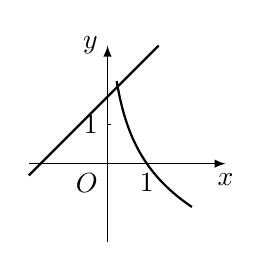
\begin{tikzpicture}[scale = 0.5,>=latex]
    \draw [->] (-2,0) -- (3,0) node [below] {$x$};
    \draw [->] (0,-2) -- (0,3) node [left] {$y$};
    \draw (0,0) node [below left] {$O$};
    \draw (0.1,1) -- (0,1) node [left] {$1$};
    \draw (1,0) node [below] {$1$};
    \draw [thick] (-2,-0.3) -- (1.3,3);
    \draw [thick,domain =-1.1:2.1,samples = 200] plot ({0.5^\x},\x);
\end{tikzpicture}
}{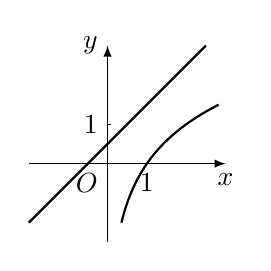
\begin{tikzpicture}[scale = 0.5,>=latex]
    \draw [->] (-2,0) -- (3,0) node [below] {$x$};
    \draw [->] (0,-2) -- (0,3) node [left] {$y$};
    \draw (0,0) node [below left] {$O$};
    \draw (0.1,1) -- (0,1) node [left] {$1$};
    \draw (1,0) node [below] {$1$};
    \draw [thick] (-2,-1.5) -- (2.5,3);
    \draw [thick,domain =1.5:-1.5,samples = 200] plot ({0.5^\x},-\x);
\end{tikzpicture}
}{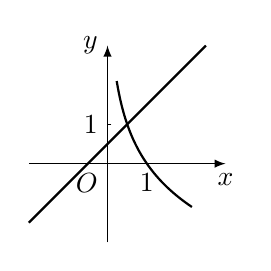
\begin{tikzpicture}[scale = 0.5,>=latex]
    \draw [->] (-2,0) -- (3,0) node [below] {$x$};
    \draw [->] (0,-2) -- (0,3) node [left] {$y$};
    \draw (0,0) node [below left] {$O$};
    \draw (0.1,1) -- (0,1) node [left] {$1$};
    \draw (1,0) node [below] {$1$};
    \draw [thick] (-2,-1.5) -- (2.5,3);
    \draw [thick,domain =-1.1:2.1,samples = 200] plot ({0.5^\x},\x);
\end{tikzpicture}
}{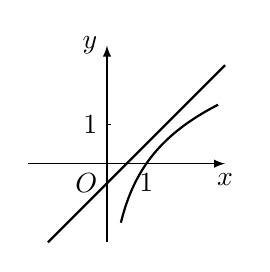
\begin{tikzpicture}[scale = 0.5,>=latex]
    \draw [->] (-2,0) -- (3,0) node [below] {$x$};
    \draw [->] (0,-2) -- (0,3) node [left] {$y$};
    \draw (0,0) node [below left] {$O$};
    \draw (0.1,1) -- (0,1) node [left] {$1$};
    \draw (1,0) node [below] {$1$};
    \draw [thick] (-1.5,-2) -- (3,2.5);
    \draw [thick,domain =1.5:-1.5,samples = 200] plot ({0.5^\x},-\x);
\end{tikzpicture}
}


关联目标:

K0211001B|D02002B|会利用指数函数的单调性解决相关不等式等问题.

K0213007B|D02002B|会作出对数函数的大致图像, 能根据其图像特征叙述函数性质.



标签: 第二单元

答案: 暂无答案

解答或提示: 暂无解答与提示

使用记录:

暂无使用记录


出处: 教材复习题
\item { (000063)}求下列函数的的定义域:\\
(1) $y=(x-1)^{\frac 52}$;\\
(2) $y=3^{\sqrt{x-1}}$;\\
(3) $y=\lg \dfrac{1+x}{1-x}$.


关联目标:

K0207002B|D02002B|会根据具体的幂指数$a$求解幂函数$y=x^{a}$的定义域.

K0209002B|D02002B|会求解有关指数型函数的定义域.

K0212002B|D02002B|会求解有关对数型函数的定义域.

K0213007B|D02002B|会作出对数函数的大致图像, 能根据其图像特征叙述函数性质.



标签: 第二单元

答案: 暂无答案

解答或提示: 暂无解答与提示

使用记录:

暂无使用记录


出处: 教材复习题
\item { (000065)}设点$(\sqrt 2, 2)$在幂函数$y_1=x^a$的图像上, 点$(-2,\dfrac 14)$在幂函数$y_2=x^b$的图像上. 当$x$取何值时, $y_1=y_2$?


关联目标:

K0207001B|D02002B|理解幂函数的定义(包含幂函数定义域的概念).



标签: 第二单元

答案: 暂无答案

解答或提示: 暂无解答与提示

使用记录:

暂无使用记录


出处: 教材复习题
\item { (000069)}填空题:\\
(1) 已知$m\in \mathbf{Z}$, 设幂函数$y=x^{m^2-4m}$的图像关于原点成中心对称, 且与$x$轴及$y$轴均无交点, 则$m$的值为\blank{50}.\\
(2) 设$a$、$b$为常数, 若$0<a<1$, $b<-1$, 则函数$y=a^x+b$的图像必定不经过第\blank{50}象限.


关联目标:

K0207004B|D02002B|会用图像上任意一点关于原点(或关于$y$轴)的对称点仍落在图像上证明函数的图像关于原点(或$y$轴)对称.

K0210002B|D02002B|知道指数函数图像过定点$(0,1)$.



标签: 第二单元

答案: 暂无答案

解答或提示: 暂无解答与提示

使用记录:

暂无使用记录


出处: 教材复习题
\item { (000070)}选择题:\\
(1) 若$m>n>1$, 而$0<x<1$, 则下列不等式正确的是\bracket{20}.
\fourch{$m^x<n^x$}{$x^m<x^n$}{$\log_x m>\log_x n$}{$\log_m x<\log_n x$}
(2) 在同一平面直角坐标系中, 二次函数$y=ax^2+bx$与指数函数$y=(\dfrac ba)^x$的图像关系可能为\bracket{20}.
\fourch{
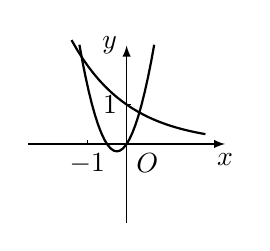
\begin{tikzpicture}[scale = 0.5, >=latex]
    \draw [->] (-2.5,0) -- (2.5,0) node [below] {$x$};
    \draw [->] (0,-2.) -- (0,2.5) node [left] {$y$};
    \draw (0,0) node [below right] {$O$};
    \draw (-1,0.1) -- (-1,0) node [below] {$-1$};
    \draw (0.1,1) -- (0,1) node [left] {$1$};
    \draw [domain = -1.2:0.7,thick] plot (\x,{3*\x * (\x+0.5)});
    \draw [domain = -1.4:2,thick] plot (\x,{(0.5)^\x}); 
\end{tikzpicture}
}{
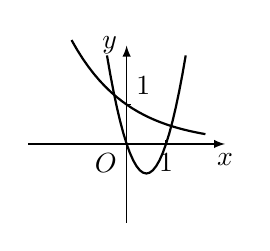
\begin{tikzpicture}[scale = 0.5, >=latex]
    \draw [->] (-2.5,0) -- (2.5,0) node [below] {$x$};
    \draw [->] (0,-2.) -- (0,2.5) node [left] {$y$};
    \draw (0,0) node [below left] {$O$};
    \draw (1,0.1) -- (1,0) node [below] {$1$};
    \draw (0.1,1) -- (0,1) node [above right] {$1$};
    \draw [domain = -0.5:1.5,thick] plot (\x,{3*\x*(\x-1)});
    \draw [domain = -1.4:2,thick] plot (\x,{(0.5)^\x}); 
\end{tikzpicture}
}{
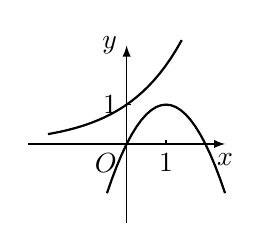
\begin{tikzpicture}[scale = 0.5, >=latex]
    \draw [->] (-2.5,0) -- (2.5,0) node [below] {$x$};
    \draw [->] (0,-2.) -- (0,2.5) node [left] {$y$};
    \draw (0,0) node [below left] {$O$};
    \draw (1,0.1) -- (1,0) node [below] {$1$};
    \draw (0.1,1) -- (0,1) node [left] {$1$};
    \draw [domain = -0.5:2.5,thick] plot ({\x},{-\x*(\x-2)});
    \draw [domain = -1.4:2,thick] plot ({-\x},{(0.5)^\x}); 
\end{tikzpicture}
}{
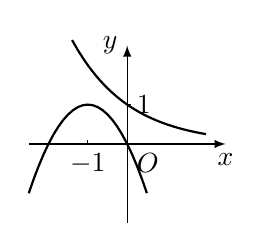
\begin{tikzpicture}[scale = 0.5, >=latex]
    \draw [->] (-2.5,0) -- (2.5,0) node [below] {$x$};
    \draw [->] (0,-2.) -- (0,2.5) node [left] {$y$};
    \draw (0,0) node [below right] {$O$};
    \draw (-1,0.1) -- (-1,0) node [below] {$-1$};
    \draw (0.1,1) -- (0,1) node [right] {$1$};
    \draw [domain = -2.5:0.5,thick] plot ({\x},{-\x*(\x+2)});
    \draw [domain = -1.4:2,thick] plot ({\x},{(0.5)^\x}); 
\end{tikzpicture}   
}


关联目标:

K0208004B|D02002B|会用幂函数的单调性判断两个幂的大小.

K0210006B|D02002B|会利用指数函数的单调性判断两个数的大小.

K0213008B|D02002B|会利用对数函数的单调性判断两个数的大小.

K0210005B|D02002B|会作出指数函数的大致图像, 能根据其图像特征叙述其函数性质.



标签: 第二单元

答案: 暂无答案

解答或提示: 暂无解答与提示

使用记录:

暂无使用记录


出处: 教材复习题
\item { (000072)}在同一平面直角坐标系中, 作出函数$y=(\dfrac 12)^x$及$y=x^{\frac 12}$的大致图像, 并求方程$(\dfrac 12)^x=x^{\frac 12}$的解的个数.


关联目标:

K0207003B|D02002B|会根据函数定义域, 利用计算器合理采点, 并能通过描点法作出幂函数$y=x^{1/2}$,$y=x^{3}$,$y=x^{-2/3}$的大致图像.

K0210005B|D02002B|会作出指数函数的大致图像, 能根据其图像特征叙述其函数性质.



标签: 第二单元

答案: 暂无答案

解答或提示: 暂无解答与提示

使用记录:

暂无使用记录


出处: 教材复习题
\item { (000076)}求函数$y=\dfrac1{2-x}+\sqrt{x^2-1}$的定义域.


关联目标:

K0215003B|D02003B|会求函数的自然定义域.



标签: 第二单元

答案: 暂无答案

解答或提示: 暂无解答与提示

使用记录:

暂无使用记录


出处: 教材复习题
\item { (000080)}分别作出下列函数的大致图像, 并指出它们的单调区间:\\
(1) $y=|x^2-4x|$;\\
(2) $y=2|x|-3$.


关联目标:

K0219001B|D02003B|理解单调函数、单调区间的定义.



标签: 第二单元

答案: 暂无答案

解答或提示: 暂无解答与提示

使用记录:

暂无使用记录


出处: 教材复习题
\item { (000083)}邮局规定: 当邮件质量不超过$100$g时, 每$20$g邮费$0.8$元, 且不足$20$g时按$20$g计算; 超过$100$g时, 超过$100$g的部分按每$100$g邮费$2$元计算, 且不足$100$g按$100$g
计算; 同时规定邮件总质量不得超过$2000$g. 请写出邮费关于邮件质量的函数表达式, 并计算$50$g和$500$g的邮件分别收多少邮费.


关联目标:

K0216005B|D02003B|了解并能根据实际情况运用函数的分段表示法.



标签: 第二单元

答案: 暂无答案

解答或提示: 暂无解答与提示

使用记录:

暂无使用记录


出处: 教材复习题
\item { (000084)}若函数$y=(a^2+4a-5)x^2-4(a-1)x+3$的图像都在$x$轴上方(不含$x$轴), 求实数$a$的取值范围.


关联目标:

K0115001B|D01004B|能通过对判别式讨论的方法解决含参一元二次(可能是一元一次, 可能不含未知数)不等式的恒成立问题.

K0223003B|D02004B|会用函数的观点求解一元二次不等式.



标签: 第二单元

答案: 暂无答案

解答或提示: 暂无解答与提示

使用记录:

暂无使用记录


出处: 教材复习题
\item { (000085)}已知$y=f(x)$是奇函数, 其定义域为$\mathbf{R}$; 而$y=g(x)$是偶函数, 其定义域为$D$. 判断函数$y=f(x)g(x)$的奇偶性, 并说明理由.


关联目标:

K0217004B|D02003B|会运用奇函数、偶函数的定义, 证明一些较为简单的函数是奇函数或是偶函数.



标签: 第二单元

答案: 暂无答案

解答或提示: 暂无解答与提示

使用记录:

暂无使用记录


出处: 教材复习题
\item { (000092)}作出函数$y=(x^2-1)^2-1$的大致图像, 写出它的单调区间, 并证明你的结论.


关联目标:

K0219001B|D02003B|理解单调函数、单调区间的定义.

K0219003B|D02003B|会运用函数单调性的定义以及已知的基本初等函数的单调性, 判断较为复杂的函数单调性.



标签: 第二单元

答案: 暂无答案

解答或提示: 暂无解答与提示

使用记录:

暂无使用记录


出处: 教材复习题
\item { (000094)}设函数$y=f(x)$, $x\in \mathbf{R}$的反函数是$y=f^{-1}(x)$.\\
(1) 如果$y=f(x)$是奇函数, 那么$y=f^{-1}(x)$的奇偶性如何?\\
(2) 如果$y=f(x)$在定义域上是严格增函数, 那么$y=f^{-1}(x)$的单调性如何?


关联目标:

K0226005B|D02004B|会探究具体函数与其反函数的基本性质之间的区别与联系.



标签: 第二单元

答案: 暂无答案

解答或提示: 暂无解答与提示

使用记录:

暂无使用记录


出处: 教材复习题
\item { (000330)}若函数$f(x)=\log_2\dfrac{x-a}{x+1}$的反函数的图像过点$(-2,3)$, 则$a=$\blank{50}.


关联目标:

暂未关联目标



标签: 第二单元

答案: $2$

解答或提示: 暂无解答与提示

使用记录:

20211119	2022届高三1班	\fcolorbox[rgb]{0,0,0}{1.000,0.094,0}{0.953}


出处: 赋能练习
\item { (000342)}若函数$f(x)=\begin{cases}    2^x, & x\le 0, \\ -x^2+m, & x>0 \end{cases}$的值域为$(-\infty ,1]$, 则实数$m$的取值范围是\blank{50}.


关联目标:

暂未关联目标



标签: 第二单元

答案: $0<m\le 1$

解答或提示: 暂无解答与提示

使用记录:

20211126	2022届高三1班	\fcolorbox[rgb]{0,0,0}{0.976,1.000,0}{0.488}

20220622	2022届高三1班  	\fcolorbox[rgb]{0,0,0}{1.000,0.140,0}{0.930}


出处: 赋能练习
\item { (000349)}若函数$f(x)=\log_2 (x+1)+a$的反函数的图像经过点$(4,1)$, 则实数$a=$\blank{50}.


关联目标:

暂未关联目标



标签: 第二单元

答案: $3$

解答或提示: 暂无解答与提示

使用记录:

20211203	2022届高三1班	\fcolorbox[rgb]{0,0,0}{1.000,0.000,0}{1.000}


出处: 赋能练习
\item { (000355)}有以下命题:\\
\textcircled{1} 若函数$f(x)$既是奇函数又是偶函数, 则$f(x)$的值域为$\{0\}$; \\
\textcircled{2} 若函数$f(x)$是偶函数, 则$f(|x|)=f(x)$;\\
\textcircled{3} 若函数$f(x)$在其定义域内不是单调函数, 则$f(x)$不存在反函数;\\
\textcircled{4} 若函数$f(x)$存在反函数${{f}^{-1}}(x)$, 且${{f}^{-1}}(x)$与$f(x)$不完全相同, 则$f(x)$与${{f}^{-1}}(x)$图像的公共点必在直线$y=x$上; \\
其中真命题的序号是\blank{50}(写出所有真命题的序号).


关联目标:

暂未关联目标



标签: 第二单元

答案: \textcircled{1}\textcircled{2}

解答或提示: 暂无解答与提示

使用记录:

20211203	2022届高三1班	\fcolorbox[rgb]{0,0,0}{1.000,0.790,0}{0.605}

20220622	2022届高三1班  	\fcolorbox[rgb]{0,0,0}{1.000,0.232,0}{0.884}


出处: 赋能练习
\item { (000381)}若点$(8,4)$在函数$f(x)=1+\log_a x$图像上, 则$f(x)$的反函数为\blank{50}.


关联目标:

暂未关联目标



标签: 第二单元

答案: $2^{x-1}$

解答或提示: 暂无解答与提示

使用记录:

20211223	2022届高三1班	\fcolorbox[rgb]{0,0,0}{1.000,0.090,0}{0.955}


出处: 赋能练习
\item { (000388)}已知函数$f(x)=a^x-1$的图像经过$(1,1)$点, 则$f^{-1}(3)=$\blank{50}.


关联目标:

暂未关联目标



标签: 第二单元

答案: $2$

解答或提示: 暂无解答与提示

使用记录:

20211230	2022届高三1班	\fcolorbox[rgb]{0,0,0}{1.000,0.000,0}{1.000}


出处: 赋能练习
\item { (000450)}函数$f(x)=2^x+m$的反函数为$y=f^{-1}(x)$, 且$y=f^{-1}(x)$的图像过点$Q(5,2)$, 那么$m=$\blank{50}.


关联目标:

暂未关联目标



标签: 第二单元

答案: $1$

解答或提示: 暂无解答与提示

使用记录:

20220221	2022届高三1班	\fcolorbox[rgb]{0,0,0}{1.000,0.000,0}{1.000}


出处: 赋能练习
\item { (000472)}若函数$f(x)=x^a$的反函数的图像经过点$(\dfrac12,\dfrac14)$, 则$a=$\blank{50}.


关联目标:

暂未关联目标



标签: 第二单元

答案: $\frac 12$

解答或提示: 暂无解答与提示

使用记录:

20220223	2022届高三1班	\fcolorbox[rgb]{0,0,0}{1.000,0.140,0}{0.930}


出处: 赋能练习
\item { (000486)}函数$f(x)=\lg(2-x)$的定义域是\blank{50}.


关联目标:

暂未关联目标



标签: 第二单元

答案: $(-\infty ,2)$

解答或提示: 暂无解答与提示

使用记录:

20220225	2022届高三1班	\fcolorbox[rgb]{0,0,0}{1.000,0.000,0}{1.000}


出处: 赋能练习
\item { (000498)}已知幂函数的图像过点$(2,\dfrac14)$, 则该幂函数的单调递增区间是\blank{50}.


关联目标:

暂未关联目标



标签: 第二单元

答案: $(-\infty ,0)$

解答或提示: 暂无解答与提示

使用记录:

20220228	2022届高三1班	\fcolorbox[rgb]{0,0,0}{1.000,0.190,0}{0.905}


出处: 赋能练习
\item { (000520)}已知函数$f(x)=a\cdot 2^x+3-a\ (a\in \mathbf{R})$的反函数为$y=f^{-1}(x)$, 则函数$y=f^{-1}(x)$的图像经过的定点的坐标为\blank{50}.


关联目标:

暂未关联目标



标签: 第二单元

答案: $(3,0)$

解答或提示: 暂无解答与提示

使用记录:

20220303	2022届高三1班	\fcolorbox[rgb]{0,0,0}{1.000,0.046,0}{0.977}


出处: 赋能练习
\item { (000567)}函数$f(x)=\sqrt{1-\lg x}$的定义域为\blank{50}.


关联目标:

K0214002B|D02002B|会利用对数函数的单调性解决其他相关不等式等数学问题和生活中的实际问题.



标签: 第二单元

答案: $(0,10 ]$

解答或提示: 暂无解答与提示

使用记录:

20220315	2022届高三1班	\fcolorbox[rgb]{0,0,0}{1.000,0.094,0}{0.953}


出处: 赋能练习
\item { (000582)}数列$\{a_n\}$的前$n$项和为$S_n$, 若点$(n,S_n) \ (n\in \mathbf{N}^*)$在函数$y=\log_2 (x+1)$的反函数的图像上, 则$a_n$=\blank{50}.


关联目标:

暂未关联目标



标签: 第二单元

答案: $a_n=2^{n-1}$

解答或提示: 暂无解答与提示

使用记录:

20220316	2022届高三1班	\fcolorbox[rgb]{0,0,0}{1.000,0.326,0}{0.837}


出处: 赋能练习
\item { (000590)}已知函数$f(x)=1+\log_a x$, $y=f^{-1}(x)$是函数$y=f(x)$的反函数, 若$y=f^{-1}(x)$的图像过点$(2,4)$, 则$a$的值为\blank{50}.


关联目标:

暂未关联目标



标签: 第二单元

答案: $4$

解答或提示: 暂无解答与提示

使用记录:

20220322	2022届高三1班	\fcolorbox[rgb]{0,0,0}{1.000,0.000,0}{1.000}


出处: 赋能练习
\item { (000607)}函数$y=\log_2(1-\dfrac1x)$的定义域为\blank{50}.


关联目标:

暂未关联目标



标签: 第二单元

答案: $(-\infty ,0)\cup (1,+\infty)$

解答或提示: 暂无解答与提示

使用记录:

20220324	2022届高三1班	\fcolorbox[rgb]{0,0,0}{1.000,0.140,0}{0.930}


出处: 赋能练习
\item { (000634)}若函数$f(x)=4^x+2^{x+1}$的图像与函数$y=g(x)$的图像关于直线$y=x$对称, 则$g(3)=$\blank{50}.


关联目标:

暂未关联目标



标签: 第二单元|第七单元

答案: $0$

解答或提示: 暂无解答与提示

使用记录:

20220329	2022届高三1班	\fcolorbox[rgb]{0,0,0}{1.000,0.046,0}{0.977}


出处: 赋能练习
\item { (000646)}函数$y=\sqrt{2x-x^2}$的定义域是\blank{50}.


关联目标:

暂未关联目标



标签: 第二单元

答案: $[0,2]$

解答或提示: 暂无解答与提示

使用记录:

20220401	2022届高三1班	\fcolorbox[rgb]{0,0,0}{1.000,0.190,0}{0.905}


出处: 赋能练习
\item { (000655)}若将函数$f(x)=|\sin(\omega x-\dfrac{\pi}8)| \ (\omega >0)$的图像向左平移$\dfrac{\pi}{12}$个单位后, 所得图像对应的函数为偶函数, 则$\omega$的最小值是\blank{50}.


关联目标:

暂未关联目标



标签: 第二单元

答案: $\dfrac 32$

解答或提示: 暂无解答与提示

使用记录:

20220401	2022届高三1班	\fcolorbox[rgb]{0,0,0}{1.000,0.380,0}{0.810}


出处: 赋能练习
\item { (000675)}已知定义在$\mathbf{R}$上的函数$f(x)$满足: \textcircled{1} $f(x)+f(2-x)=0$; \textcircled{2} $f(x)-f(-2-x)=0$; \textcircled{3} 在$[-1,1]$上的表达式为$f(x)=\begin{cases} \sqrt{1-x^2}, & x\in [-1,0], \\ 1-x, & x\in (0,1] \end{cases}$, 则函数$f(x)$与函数$g(x)=\begin{cases} 2^x, & x\le 0, \\ \log_{\frac12} x,& x>0 \end{cases}$的图像在区间$[-3,3]$上的交点的个数为\blank{50}.


关联目标:

暂未关联目标



标签: 第二单元

答案: $6$

解答或提示: 暂无解答与提示

使用记录:

20220408	2022届高三1班	\fcolorbox[rgb]{0,0,0}{1.000,0.418,0}{0.791}


出处: 赋能练习
\item { (000715)}设奇函数$f(x)$的定义域为$\mathbf{R}$, 当$x>0$时,$f(x)=x+\dfrac{m^2}x-1$(这里$m$为正常数). 若$f(x)\le m-2$对一切$x\le 0$成立, 则$m$的取值范围为\blank{50}.


关联目标:

暂未关联目标



标签: 第二单元

答案: $[2,+\infty)$

解答或提示: 暂无解答与提示

使用记录:

20220422	2022届高三1班	\fcolorbox[rgb]{0,0,0}{1.000,0.976,0}{0.512}

20220622	2022届高三1班  	\fcolorbox[rgb]{0,0,0}{1.000,0.186,0}{0.907}


出处: 赋能练习
\item { (000738)}函数$f(x)=\lg (3^x-2^x)$的定义域为\blank{50}.


关联目标:

K0211001B|D02002B|会利用指数函数的单调性解决相关不等式等问题.

K0212002B|D02002B|会求解有关对数型函数的定义域.



标签: 第二单元

答案: $(0,+\infty)$

解答或提示: 暂无解答与提示

使用记录:

20220427	2022届高三1班	\fcolorbox[rgb]{0,0,0}{1.000,0.280,0}{0.860}


出处: 赋能练习
\item { (000758)}若函数$f(x)=\sqrt{8-ax-2x^2}$是偶函数, 则该函数的定义域是\blank{50}.


关联目标:

暂未关联目标



标签: 第二单元

答案: $[-2,2]$

解答或提示: 暂无解答与提示

使用记录:

20220506	2022届高三1班	\fcolorbox[rgb]{0,0,0}{1.000,0.000,0}{1.000}


出处: 赋能练习
\item { (000778)}函数$y=\sqrt{\lg(x+2)}$的定义域为\blank{50}.


关联目标:

暂未关联目标



标签: 第二单元

答案: $\{x|x\ge -1\}$

解答或提示: 暂无解答与提示

使用记录:

20220510	2022届高三1班	\fcolorbox[rgb]{0,0,0}{1.000,0.046,0}{0.977}


出处: 赋能练习
\item { (000845)}已知函数$f(x)=\lg (\sqrt{x^2+1}+ax)$的定义域为$\mathbf{R}$, 则实数$a$的取值范围是\blank{50}.


关联目标:

暂未关联目标



标签: 第二单元

答案: $[-1, 1]$

解答或提示: 暂无解答与提示

使用记录:

20220525	2022届高三1班	\fcolorbox[rgb]{0,0,0}{1.000,0.094,0}{0.953}


出处: 赋能练习
\item { (000851)}已知函数$f(x)=\dfrac{3x+1}{x+a}\ (a\ne \dfrac13)$的图像与它的反函数的图像重合, 则实数$a$的值为\blank{50}.


关联目标:

暂未关联目标



标签: 第二单元

答案: $a=-3$

解答或提示: 暂无解答与提示

使用记录:

20220526	2022届高三1班	\fcolorbox[rgb]{0,0,0}{1.000,0.140,0}{0.930}


出处: 赋能练习
\item { (000859)}设$a>0$且$a\ne 1$, 若函数$f(x)=a^{x-1}+2$的反函数的图像经过定点$P$, 则点$P$的坐标是\blank{50}.


关联目标:

暂未关联目标



标签: 第二单元

答案: $(3,1)$

解答或提示: 暂无解答与提示

使用记录:

20220527	2022届高三1班	\fcolorbox[rgb]{0,0,0}{1.000,0.186,0}{0.907}


出处: 赋能练习
\item { (000868)}函数$f(x)=\dfrac{\sqrt{x+2}}{x-1}$的定义域为\blank{50}.


关联目标:

暂未关联目标



标签: 第二单元

答案: $[-2,1)\cup (1,+\infty)$

解答或提示: 暂无解答与提示

使用记录:

20220601	2022届高三1班	\fcolorbox[rgb]{0,0,0}{1.000,0.094,0}{0.953}


出处: 赋能练习
\item { (000931)}函数$y=\log_3 (x-1)$的定义域是\blank{50}.


关联目标:

暂未关联目标



标签: 第二单元

答案: $(1,+\infty)$

解答或提示: 暂无解答与提示

使用记录:

20220622	2022届高三1班	\fcolorbox[rgb]{0,0,0}{1.000,0.000,0}{1.000}


出处: 赋能练习
\item { (000949)}已知函数$f(x)={x^3}+\lg (\sqrt{x^2+1}+x)$, 若$f(x)$的定义域中的$a$、$b$满足$f(-a)+f(-b)-3=f(a)+f(b)+3$, 则$f(a)+f(b)=$\blank{50}.


关联目标:

暂未关联目标



标签: 第二单元

答案: $-3$

解答或提示: 暂无解答与提示

使用记录:

20220624	2022届高三1班	\fcolorbox[rgb]{0,0,0}{1.000,0.046,0}{0.977}


出处: 赋能练习
\item { (000954)}函数$y=\sqrt{2^x-1}$的定义域是\blank{50}(用区间表示).


关联目标:

K0211001B|D02002B|会利用指数函数的单调性解决相关不等式等问题.



标签: 第二单元

答案: $[0,+\infty)$

解答或提示: 暂无解答与提示

使用记录:

20220628	2022届高三1班	\fcolorbox[rgb]{0,0,0}{1.000,0.000,0}{1.000}


出处: 赋能练习
\item { (000961)}已知函数$f(x)=2^x-a\cdot 2^{-x}$的反函数是$f^{-1}(x)$, $f^{-1}(x)$在定义域上是奇函数, 则正实数$a=$\blank{50}.


关联目标:

暂未关联目标



标签: 第二单元

答案: $a=1$

解答或提示: 暂无解答与提示

使用记录:

20220628	2022届高三1班	\fcolorbox[rgb]{0,0,0}{1.000,0.000,0}{1.000}


出处: 赋能练习
\item { (001160)}已知函数$f(x)=3x+5, \ x\in \mathbf{R}$, 求$f(-1)$, $f(10)$, $f(a)$, $f(a^2+1)$. 并写出函数$y=f(f(x))$的定义域, 对应法则以及值域.


关联目标:

暂未关联目标



标签: 第二单元

答案: 暂无答案

解答或提示: 暂无解答与提示

使用记录:

2016届11班	\fcolorbox[rgb]{0,0,0}{1.000,0.210,0}{0.895}

2016届12班	\fcolorbox[rgb]{0,0,0}{1.000,0.316,0}{0.842}


出处: 2016届创新班作业	1131-函数与函数的三要素
\item { (001161)}下列两个函数是同一个函数的有\blank{50}.\\ 
(1) $y=\dfrac{x^2-1}{x-1}$与$y=x+1$;\\ 
(2) $y=\dfrac{x^3}{x}$与$y=x^2$;\\ 
(3) $y=\sqrt{x^2}-1$与$y=\sqrt[3]{x^3}-1$;\\ 
(4) $f(x)=x^2-2x-1$与$g(t)=t^2-2t-1$;\\ 
(5) $f(x)=2^x, \ x \in \{0,1,2,3\}$与$g(x)=\dfrac16x^3+\dfrac56x+1, \ x \in \{0,1,2,3\}$.


关联目标:

暂未关联目标



标签: 第二单元

答案: 暂无答案

解答或提示: 暂无解答与提示

使用记录:

2016届11班	\fcolorbox[rgb]{0,0,0}{1.000,0.106,0}{0.947}

2016届12班	\fcolorbox[rgb]{0,0,0}{1.000,0.210,0}{0.895}


出处: 2016届创新班作业	1131-函数与函数的三要素
\item { (001164)}写出下列函数的定义域(写在对应关系的右边):\\ 
(1) $f(x)=\dfrac{6}{x^2-3x+2}$;\\ 
(2) $f(x)=\dfrac{3x-1}{2x^3+4x^2+x-7}$;\\ 
(3) $f(x)=\dfrac{\sqrt[3]{4x+8}}{\sqrt{3x-2}}$;\\ 
(4) $f(x)=\sqrt{2x-1}+\sqrt{1-2x}+4$;\\ 
(5) $f(x)=\sqrt{x^2-4}$;\\ 
(6) $f(x)=\dfrac{\sqrt{2x+1}}{x-3}$.


关联目标:

暂未关联目标



标签: 第二单元

答案: 暂无答案

解答或提示: 暂无解答与提示

使用记录:

2016届11班	\fcolorbox[rgb]{0,0,0}{1.000,0.158,0}{0.921}	\fcolorbox[rgb]{0,0,0}{1.000,0.210,0}{0.895}	\fcolorbox[rgb]{0,0,0}{1.000,0.052,0}{0.974}	\fcolorbox[rgb]{0,0,0}{1.000,0.264,0}{0.868}	\fcolorbox[rgb]{0,0,0}{1.000,0.158,0}{0.921}	\fcolorbox[rgb]{0,0,0}{1.000,0.000,0}{1.000}

2016届12班	\fcolorbox[rgb]{0,0,0}{1.000,0.264,0}{0.868}	\fcolorbox[rgb]{0,0,0}{1.000,0.368,0}{0.816}	\fcolorbox[rgb]{0,0,0}{1.000,0.210,0}{0.895}	\fcolorbox[rgb]{0,0,0}{1.000,0.526,0}{0.737}	\fcolorbox[rgb]{0,0,0}{1.000,0.316,0}{0.842}	\fcolorbox[rgb]{0,0,0}{1.000,0.210,0}{0.895}


出处: 2016届创新班作业	1131-函数与函数的三要素
\item { (001165)}(1) 函数$f(x)=x^2, \ x \in [0,1]$的值域为\blank{50};\\ 
(2) 函数$f(x)=-x, \ x \in [-1,0)$的值域为\blank{50};\\ 
(3) 函数$f(x)=\left\{\begin{array}{cc}x^2,&0\le x\le 1,\\-x,&-1\le x<0.\end{array}\right.$的值域为\blank{50}.


关联目标:

暂未关联目标



标签: 第二单元

答案: 暂无答案

解答或提示: 暂无解答与提示

使用记录:

2016届11班	\fcolorbox[rgb]{0,0,0}{1.000,0.052,0}{0.974}	\fcolorbox[rgb]{0,0,0}{1.000,0.106,0}{0.947}	\fcolorbox[rgb]{0,0,0}{1.000,0.052,0}{0.974}

2016届12班	\fcolorbox[rgb]{0,0,0}{1.000,0.052,0}{0.974}	\fcolorbox[rgb]{0,0,0}{1.000,0.052,0}{0.974}	\fcolorbox[rgb]{0,0,0}{1.000,0.158,0}{0.921}


出处: 2016届创新班作业	1131-函数与函数的三要素
\item { (001166)}函数$f(x)=\sqrt{kx^2+4kx+3}$的定义域为$\mathbf{R}$, 求实数$k$的取值范围.


关联目标:

暂未关联目标



标签: 第二单元

答案: 暂无答案

解答或提示: 暂无解答与提示

使用记录:

2016届11班	\fcolorbox[rgb]{0,0,0}{0.948,1.000,0}{0.474}

2016届12班	\fcolorbox[rgb]{0,0,0}{1.000,1.000,0}{0.500}


出处: 2016届创新班作业	1131-函数与函数的三要素
\item { (001167)}求函数$y=x^3+1$的值域(要详细过程).


关联目标:

暂未关联目标



标签: 第二单元

答案: 暂无答案

解答或提示: 暂无解答与提示

使用记录:

2016届11班	\fcolorbox[rgb]{0,0,0}{1.000,0.526,0}{0.737}

2016届12班	\fcolorbox[rgb]{0,0,0}{1.000,0.368,0}{0.816}


出处: 2016届创新班作业	1131-函数与函数的三要素
\item { (001173)}在以下坐标系中分别作出下列函数的图像(用铅笔, 要求清晰, 交代关键信息):\\ 
\begin{tabular}{ll}
(1) $y=\sqrt{|x|}$;& (2) $y=|x-1|-|x+1|$;\\
\begin{tikzpicture}[>=latex]
    \foreach \i in {-4,-3,...,4} {\draw [dashed, gray!90] (-4,\i) -- (4,\i) (\i,-4) -- (\i,4);};
    \draw [->] (-4,0) -- (4,0) node [below] {$x$};
    \draw [->] (0,-4) -- (0,4) node [left] {$y$};
    \draw (0,0) node [below left] {$O$};
    \draw (0,1) node [left] {$1$};
    \draw (1,0) node [below] {$1$};
\end{tikzpicture} & 
\begin{tikzpicture}[>=latex]
    \foreach \i in {-4,-3,...,4} {\draw [dashed, gray!90] (-4,\i) -- (4,\i) (\i,-4) -- (\i,4);};
    \draw [->] (-4,0) -- (4,0) node [below] {$x$};
    \draw [->] (0,-4) -- (0,4) node [left] {$y$};
    \draw (0,0) node [below left] {$O$};
    \draw (0,1) node [left] {$1$};
    \draw (1,0) node [below] {$1$};
\end{tikzpicture}
\end{tabular}
\begin{tabular}{ll}
(3) $y=x-[x]$;& (4) $y=x+\dfrac{1}{x}$;\\
\begin{tikzpicture}[>=latex]
    \foreach \i in {-4,-3,...,4} {\draw [dashed, gray!90] (-4,\i) -- (4,\i) (\i,-4) -- (\i,4);};
    \draw [->] (-4,0) -- (4,0) node [below] {$x$};
    \draw [->] (0,-4) -- (0,4) node [left] {$y$};
    \draw (0,0) node [below left] {$O$};
    \draw (0,1) node [left] {$1$};
    \draw (1,0) node [below] {$1$};
\end{tikzpicture} & 
\begin{tikzpicture}[>=latex]
    \foreach \i in {-4,-3,...,4} {\draw [dashed, gray!90] (-4,\i) -- (4,\i) (\i,-4) -- (\i,4);};
    \draw [->] (-4,0) -- (4,0) node [below] {$x$};
    \draw [->] (0,-4) -- (0,4) node [left] {$y$};
    \draw (0,0) node [below left] {$O$};
    \draw (0,1) node [left] {$1$};
    \draw (1,0) node [below] {$1$};
\end{tikzpicture}
\end{tabular}
\begin{tabular}{ll}
(5) $y=x-\dfrac{1}{x}$;& (6) $y=\dfrac{6x}{1+x^2}$.\\
\begin{tikzpicture}[>=latex]
    \foreach \i in {-4,-3,...,4} {\draw [dashed, gray!90] (-4,\i) -- (4,\i) (\i,-4) -- (\i,4);};
    \draw [->] (-4,0) -- (4,0) node [below] {$x$};
    \draw [->] (0,-4) -- (0,4) node [left] {$y$};
    \draw (0,0) node [below left] {$O$};
    \draw (0,1) node [left] {$1$};
    \draw (1,0) node [below] {$1$};
\end{tikzpicture} & 
\begin{tikzpicture}[>=latex]
    \foreach \i in {-4,-3,...,4} {\draw [dashed, gray!90] (-4,\i) -- (4,\i) (\i,-4) -- (\i,4);};
    \draw [->] (-4,0) -- (4,0) node [below] {$x$};
    \draw [->] (0,-4) -- (0,4) node [left] {$y$};
    \draw (0,0) node [below left] {$O$};
    \draw (0,1) node [left] {$1$};
    \draw (1,0) node [below] {$1$};
\end{tikzpicture}
\end{tabular}


关联目标:

暂未关联目标



标签: 第二单元

答案: 暂无答案

解答或提示: 暂无解答与提示

使用记录:

2016届11班	\fcolorbox[rgb]{0,0,0}{1.000,0.052,0}{0.974}	\fcolorbox[rgb]{0,0,0}{1.000,0.000,0}{1.000}	\fcolorbox[rgb]{0,0,0}{1.000,0.106,0}{0.947}	\fcolorbox[rgb]{0,0,0}{1.000,0.264,0}{0.868}	\fcolorbox[rgb]{0,0,0}{1.000,0.210,0}{0.895}	\fcolorbox[rgb]{0,0,0}{1.000,0.736,0}{0.632}

2016届12班	\fcolorbox[rgb]{0,0,0}{1.000,0.158,0}{0.921}	\fcolorbox[rgb]{0,0,0}{1.000,0.052,0}{0.974}	\fcolorbox[rgb]{0,0,0}{1.000,0.106,0}{0.947}	\fcolorbox[rgb]{0,0,0}{1.000,0.368,0}{0.816}	\fcolorbox[rgb]{0,0,0}{1.000,0.158,0}{0.921}	\fcolorbox[rgb]{0,0,0}{1.000,0.894,0}{0.553}


出处: 2016届创新班作业	1133-函数的图像
\item { (001174)}某种茶杯每个$0.5$元, 买$x$个茶杯的钱数为$y$元. 画出$y$关于$x$的函数的图像.\\ 
\begin{tikzpicture}[>=latex]
    \foreach \i in {0,1,...,7} {\draw [dashed, gray!90] (0,\i) -- (16,\i);};
    \foreach \i in {0,1,...,16} {\draw [dashed, gray!90] (\i,0) -- (\i,7);};
    \draw [->] (-0.5,0) -- (16,0) node [below] {$x$};
    \draw [->] (0,-0.5) -- (0,7) node [left] {$y$};
    \draw (0,0) node [below left] {$O$};
    \draw (0,1) node [left] {$1$};
    \draw (1,0) node [below] {$1$};
\end{tikzpicture}


关联目标:

暂未关联目标



标签: 第二单元

答案: 暂无答案

解答或提示: 暂无解答与提示

使用记录:

2016届11班	\fcolorbox[rgb]{0,0,0}{1.000,0.210,0}{0.895}

2016届12班	\fcolorbox[rgb]{0,0,0}{1.000,0.684,0}{0.658}


出处: 2016届创新班作业	1133-函数的图像
\item { (001175)}证明: 函数$y=\dfrac{1}{x}$的图像关于原点对称(一个图形关于原点对称是指任取该图形上的一点, 它关于原点对称所得的点也在该图形上).


关联目标:

暂未关联目标



标签: 第二单元

答案: 暂无答案

解答或提示: 暂无解答与提示

使用记录:

2016届11班	\fcolorbox[rgb]{0,0,0}{1.000,0.158,0}{0.921}

2016届12班	\fcolorbox[rgb]{0,0,0}{1.000,0.106,0}{0.947}


出处: 2016届创新班作业	1133-函数的图像
\item { (001176)}求证: 函数$y=x^3$的图像不是一条直线(本题不能使用斜率的概念).


关联目标:

暂未关联目标



标签: 第二单元

答案: 暂无答案

解答或提示: 暂无解答与提示

使用记录:

2016届11班	\fcolorbox[rgb]{0,0,0}{0.842,1.000,0}{0.421}

2016届12班	\fcolorbox[rgb]{0,0,0}{1.000,1.000,0}{0.500}


出处: 2016届创新班作业	1133-函数的图像
\item { (001177)}试求出函数$y=x^2$的图像分别进行如下变换后, 所得的各个图像对应的函数.\\ 
(1) 向右平移$2$个单位;\\ 
(2) 向上平移$1$个单位;\\ 
(3) 先向右平移$2$个单位, 再向上平移$1$个单位;\\ 
(4) 先向上平移$1$个单位, 再向右平移$2$个单位


关联目标:

暂未关联目标



标签: 第二单元

答案: 暂无答案

解答或提示: 暂无解答与提示

使用记录:

2016届11班	\fcolorbox[rgb]{0,0,0}{1.000,0.000,0}{1.000}	\fcolorbox[rgb]{0,0,0}{1.000,0.000,0}{1.000}	\fcolorbox[rgb]{0,0,0}{1.000,0.000,0}{1.000}	\fcolorbox[rgb]{0,0,0}{1.000,0.000,0}{1.000}

2016届12班	\fcolorbox[rgb]{0,0,0}{1.000,0.106,0}{0.947}	\fcolorbox[rgb]{0,0,0}{1.000,0.052,0}{0.974}	\fcolorbox[rgb]{0,0,0}{1.000,0.000,0}{1.000}	\fcolorbox[rgb]{0,0,0}{1.000,0.000,0}{1.000}


出处: 2016届创新班作业	1134-函数图像的平移与放缩
\item { (001178)}试求出函数$y=\sqrt{x}$的图像分别进行如下变换后所得的各个图像对应的函数.\\ 
(1) 图像上的每一点的横坐标变为原来的$2$倍;\\ 
(2) 图像上的每一点的纵坐标变为原来的$\dfrac{1}{2}$;\\ 
(3) 图像上的每一点的横坐标变为原来的$2$倍, 然后向上平移$3$个单位, 所得图像上每一点的纵坐标变为原来的$3$倍, 再向左平移$2$个单位;\\ 
(4) 向左平移$3$个单位, 然后将所得图像上的每一点的横坐标变为原来的$\dfrac{1}{2}$, 最后向下平移$2$个单位


关联目标:

暂未关联目标



标签: 第二单元

答案: 暂无答案

解答或提示: 暂无解答与提示

使用记录:

2016届11班	\fcolorbox[rgb]{0,0,0}{1.000,0.000,0}{1.000}	\fcolorbox[rgb]{0,0,0}{1.000,0.106,0}{0.947}	\fcolorbox[rgb]{0,0,0}{1.000,0.368,0}{0.816}	\fcolorbox[rgb]{0,0,0}{1.000,0.106,0}{0.947}

2016届12班	\fcolorbox[rgb]{0,0,0}{1.000,0.052,0}{0.974}	\fcolorbox[rgb]{0,0,0}{1.000,0.106,0}{0.947}	\fcolorbox[rgb]{0,0,0}{1.000,0.264,0}{0.868}	\fcolorbox[rgb]{0,0,0}{1.000,0.632,0}{0.684}


出处: 2016届创新班作业	1134-函数图像的平移与放缩
\item { (001179)}欲将函数$y=3x$的图像通过一次平移变为函数$y=3x-5$的图像, 可向\blank{50}平移\blank{50}个单位; 也可向\blank{50}平移\blank{50}个单位.


关联目标:

暂未关联目标



标签: 第二单元

答案: 暂无答案

解答或提示: 暂无解答与提示

使用记录:

2016届11班	\fcolorbox[rgb]{0,0,0}{1.000,0.000,0}{1.000}

2016届12班	\fcolorbox[rgb]{0,0,0}{1.000,0.000,0}{1.000}


出处: 2016届创新班作业	1134-函数图像的平移与放缩
\item { (001180)}欲将函数$y=x^2$的图像通过平移和放缩变为函数$y=2x^2-4x-1$的图像, 所需的步骤依次为: (同时写出每步变换后所得图像对应的函数)


关联目标:

暂未关联目标



标签: 第二单元

答案: 暂无答案

解答或提示: 暂无解答与提示

使用记录:

2016届11班	\fcolorbox[rgb]{0,0,0}{1.000,0.632,0}{0.684}

2016届12班	\fcolorbox[rgb]{0,0,0}{1.000,0.368,0}{0.816}


出处: 2016届创新班作业	1134-函数图像的平移与放缩
\item { (001181)}证明: 在平面直角坐标系中, 将函数$y=f(x),x\in \mathbf{R}$的图像绕原点旋转$180^\circ$, 得到的是函数$y=-f(-x),x\in \mathbf{R}$的图像.


关联目标:

暂未关联目标



标签: 第二单元

答案: 暂无答案

解答或提示: 暂无解答与提示

使用记录:

2016届11班	\fcolorbox[rgb]{0,0,0}{1.000,0.158,0}{0.921}

2016届12班	\fcolorbox[rgb]{0,0,0}{1.000,0.158,0}{0.921}


出处: 2016届创新班作业	1134-函数图像的平移与放缩
\item { (001182)}在平面直角坐标系中, 将函数$y=f(x),x\in \mathbf{R}$的图像沿直线$x=1$翻折, 将会得到哪个函数的图像? 试写出这个函数, 并证明.


关联目标:

暂未关联目标



标签: 第二单元

答案: 暂无答案

解答或提示: 暂无解答与提示

使用记录:

2016届11班	\fcolorbox[rgb]{0,0,0}{1.000,0.422,0}{0.789}

2016届12班	\fcolorbox[rgb]{0,0,0}{1.000,0.422,0}{0.789}


出处: 2016届创新班作业	1134-函数图像的平移与放缩
\item { (001185)}已知$f(x)=x^2$, $g(x)=\dfrac{1}{x}$.\\ 
(1) 求$f(x)+g(x)$, $f(x)g(x)$和$\dfrac{f(x)}{g(x)}$;\\ 
(2) 求$f\circ g$和$g\circ f$;\\ 
(3) 求$f\circ g-g\circ f$, 判断它是否在其定义域上恒等于零.


关联目标:

暂未关联目标



标签: 第二单元

答案: 暂无答案

解答或提示: 暂无解答与提示

使用记录:

2016届11班	\fcolorbox[rgb]{0,0,0}{1.000,0.000,0}{1.000}	\fcolorbox[rgb]{0,0,0}{1.000,0.102,0}{0.949}	\fcolorbox[rgb]{0,0,0}{1.000,0.410,0}{0.795}

2016届12班	\fcolorbox[rgb]{0,0,0}{1.000,0.000,0}{1.000}	\fcolorbox[rgb]{0,0,0}{1.000,0.000,0}{1.000}	\fcolorbox[rgb]{0,0,0}{1.000,0.842,0}{0.579}


出处: 2016届创新班作业	1135-函数的运算与复合
\item { (001186)}已知$f(x)=x^2$, $g(x)=\dfrac{1}{x+1}$.\\ 
(1) 求$f(x)+g(x)$, $f(x)g(x)$和$\dfrac{f(x)}{g(x)}$;\\ 
(2) 求$f\circ g$和$g\circ f$;\\ 
(3) 求$f\circ g-g\circ f$, 判断它是否在其定义域上恒等于零.


关联目标:

暂未关联目标



标签: 第二单元

答案: 暂无答案

解答或提示: 暂无解答与提示

使用记录:

2016届11班	\fcolorbox[rgb]{0,0,0}{1.000,0.102,0}{0.949}	\fcolorbox[rgb]{0,0,0}{1.000,0.462,0}{0.769}	\fcolorbox[rgb]{0,0,0}{1.000,0.820,0}{0.590}

2016届12班	\fcolorbox[rgb]{0,0,0}{1.000,0.158,0}{0.921}	\fcolorbox[rgb]{0,0,0}{1.000,0.052,0}{0.974}	\fcolorbox[rgb]{0,0,0}{0.894,1.000,0}{0.447}


出处: 2016届创新班作业	1135-函数的运算与复合
\item { (001190)}下列各映射中, 是单射的有\blank{60}, 是满射的有\blank{60}, 存在逆映射的有\blank{60}.\\ 
\textcircled{1} $f: \{1,2,3\}\rightarrow \{1,4,9\}; \ x\mapsto x^2$;\\ 
\textcircled{2} $f: \mathbf{R}^+\rightarrow \mathbf{R}^+; \ x \mapsto x^2$;\\ 
\textcircled{3} $f: \mathbf{R}\rightarrow [0,+\infty); \ x \mapsto x^2$;\\ 
\textcircled{4} $f: \mathbf{R}^+\rightarrow \mathbf{R}^+; \ x \mapsto \dfrac{1}{x}$;\\ 
\textcircled{5} $f: \mathbf{R}^+\cup \mathbf{R}^-\rightarrow \mathbf{R}^+\cup \mathbf{R}^-; \ x \mapsto \dfrac{1}{x}$;\\ 
\textcircled{6} $f: \mathbf{R}^+\rightarrow \mathbf{R}; \ x \mapsto x+\dfrac{1}{x}$;\\ 
\textcircled{7} $f: \mathbf{R}^+\rightarrow \mathbf{R}; \ x \mapsto x-\dfrac{1}{x}$;\\ 
\textcircled{8} $f: \mathbf{R}\rightarrow \mathbf{Z}; \ x \mapsto [x]$;\\ 
\textcircled{9} $f: \{(x,y)|x,y\in \mathbf{R}\}\rightarrow \{(x,y)|x,y\in \mathbf{R}\};\ (x,y)\mapsto (x+y,x-y)$;\\ 
\textcircled{10} $f: \{(x,y)|x,y\in \mathbf{R}\}\rightarrow \{(x,y)|x,y\in \mathbf{R}\};\ (x,y)\mapsto (x+y,2x+2y)$.


关联目标:

暂未关联目标



标签: 第二单元

答案: 暂无答案

解答或提示: 暂无解答与提示

使用记录:

2016届11班	\fcolorbox[rgb]{0,0,0}{0.410,1.000,0}{0.205}

2016届12班	\fcolorbox[rgb]{0,0,0}{0.474,1.000,0}{0.237}


出处: 2016届创新班作业	1136-逆映射与反函数
\item { (001192)}写出下列函数的反函数(注意定义域).\\ 
(1) $y=-\dfrac{1}{x}+3$;\\ 
(2) $y=\sqrt{2x-1}$;\\ 
(3) $y=\dfrac{2x+1}{x+2}$;\\ 
(4) $y=x^2+2, \ x\in [2,+\infty)$;\\ 
(5) $y=2^x, \ x\in \{1,2,3,4\}$ (本小题不能使用对数);\\ 
(6) $y=\sqrt{9-x^2}, \ x\in [-3,0]$;\\ 
(7) $y=x^2-4x, x \in [3,7]$.


关联目标:

暂未关联目标



标签: 第二单元

答案: 暂无答案

解答或提示: 暂无解答与提示

使用记录:

2016届11班	\fcolorbox[rgb]{0,0,0}{1.000,0.102,0}{0.949}	\fcolorbox[rgb]{0,0,0}{1.000,0.154,0}{0.923}	\fcolorbox[rgb]{0,0,0}{1.000,0.154,0}{0.923}	\fcolorbox[rgb]{0,0,0}{1.000,0.102,0}{0.949}	\fcolorbox[rgb]{0,0,0}{1.000,0.462,0}{0.769}	\fcolorbox[rgb]{0,0,0}{1.000,0.974,0}{0.513}	\fcolorbox[rgb]{0,0,0}{1.000,0.256,0}{0.872}

2016届12班	\fcolorbox[rgb]{0,0,0}{1.000,0.052,0}{0.974}	\fcolorbox[rgb]{0,0,0}{1.000,0.158,0}{0.921}	\fcolorbox[rgb]{0,0,0}{1.000,0.264,0}{0.868}	\fcolorbox[rgb]{0,0,0}{1.000,0.052,0}{0.974}	\fcolorbox[rgb]{0,0,0}{1.000,0.894,0}{0.553}	\fcolorbox[rgb]{0,0,0}{0.790,1.000,0}{0.395}	\fcolorbox[rgb]{0,0,0}{1.000,0.210,0}{0.895}


出处: 2016届创新班作业	1136-逆映射与反函数
\item { (001193)}已知函数$y=f(x)$的图像经过$(1,2)$, 它有反函数$y=f^{-1}(x)$. 那么函数$y=f^{-1}(x+3)$的图像一定经过点\blank{50}.


关联目标:

暂未关联目标



标签: 第二单元

答案: 暂无答案

解答或提示: 暂无解答与提示

使用记录:

2016届11班	\fcolorbox[rgb]{0,0,0}{1.000,0.256,0}{0.872}

2016届12班	\fcolorbox[rgb]{0,0,0}{1.000,0.316,0}{0.842}


出处: 2016届创新班作业	1136-逆映射与反函数
\item { (001194)}已知函数$y=f(x)$有反函数, 且$y=f^{-1}(3x+1)$的图像经过点$(0,-1)$. 试确定函数$y=5f(x+2)+3$的图像一定经过的点, 并说明理由.


关联目标:

暂未关联目标



标签: 第二单元

答案: 暂无答案

解答或提示: 暂无解答与提示

使用记录:

2016届11班	\fcolorbox[rgb]{0,0,0}{1.000,0.666,0}{0.667}

2016届12班	\fcolorbox[rgb]{0,0,0}{0.948,1.000,0}{0.474}


出处: 2016届创新班作业	1136-逆映射与反函数
\item { (001196)}已知函数$y=f(x)$的图像经过第一, 第二象限, 且它有反函数$y=f^{-1}(x)$. 那么$y=f^{-1}(x)$的图像一定经过\blank{80}象限.


关联目标:

暂未关联目标



标签: 第二单元

答案: 暂无答案

解答或提示: 暂无解答与提示

使用记录:

2016届11班	\fcolorbox[rgb]{0,0,0}{1.000,0.102,0}{0.949}

2016届12班	\fcolorbox[rgb]{0,0,0}{1.000,0.054,0}{0.973}


出处: 2016届创新班作业	1137-函数图像综合练习
\item { (001198)}在同一坐标系中通过平移和放缩作出以下函数的图像, 并写出变换的方法.
$y=|x|$; $y=|x-1|$; $y=\dfrac{|x-1|}2$; $y=\dfrac{|x-1|}2-3$; $y=\dfrac{|2x-1|}2-3$.
\begin{center}
\begin{tikzpicture}[>=latex]
    \foreach \i in {-4,-3,...,4} {\draw [dashed, gray!90] (-4,\i) -- (4,\i) (\i,-4) -- (\i,4);};
    \draw [->] (-4,0) -- (4,0) node [below] {$x$};
    \draw [->] (0,-4) -- (0,4) node [left] {$y$};
    \draw (0,0) node [below left] {$O$};
    \draw (0,1) node [left] {$1$};
    \draw (1,0) node [below] {$1$};
\end{tikzpicture}
\end{center}


关联目标:

暂未关联目标



标签: 第二单元

答案: 暂无答案

解答或提示: 暂无解答与提示

使用记录:

2016届11班	\fcolorbox[rgb]{0,0,0}{1.000,0.358,0}{0.821}

2016届12班	\fcolorbox[rgb]{0,0,0}{1.000,0.648,0}{0.676}


出处: 2016届创新班作业	1137-函数图像综合练习
\item { (001199)}(1)欲将函数$y=x^2$的图像通过先平移后放缩的方式变为函数$y=\dfrac{1}{2}x^2+x$的图像, 所需的步骤依次为: (同时写出每步变换后所得图像对应的函数)\\ 
(2)欲将函数$y=x^2$的图像通过先放缩后平移的方式变为函数$y=\dfrac{1}{2}x^2+x$的图像, 所需的步骤依次为: (同时写出每步变换后所得图像对应的函数)


关联目标:

暂未关联目标



标签: 第二单元

答案: 暂无答案

解答或提示: 暂无解答与提示

使用记录:

2016届11班	\fcolorbox[rgb]{0,0,0}{1.000,0.154,0}{0.923}	\fcolorbox[rgb]{0,0,0}{1.000,0.154,0}{0.923}

2016届12班	\fcolorbox[rgb]{0,0,0}{1.000,0.108,0}{0.946}	\fcolorbox[rgb]{0,0,0}{1.000,0.054,0}{0.973}


出处: 2016届创新班作业	1137-函数图像综合练习
\item { (001200)}(1)欲将函数$y=\sqrt{x}$的图像通过先平移后放缩的方式变为函数$y=\sqrt{2x-4}$的图像, 所需的步骤依次为: (同时写出每步变换后所得图像对应的函数)\\ 
(2)欲将函数$y=\sqrt{x}$的图像通过先放缩后平移的方式变为函数$y=\sqrt{2x-4}$的图像, 所需的步骤依次为: (同时写出每步变换后所得图像对应的函数)


关联目标:

暂未关联目标



标签: 第二单元

答案: 暂无答案

解答或提示: 暂无解答与提示

使用记录:

2016届11班	\fcolorbox[rgb]{0,0,0}{1.000,0.000,0}{1.000}	\fcolorbox[rgb]{0,0,0}{1.000,0.256,0}{0.872}

2016届12班	\fcolorbox[rgb]{0,0,0}{1.000,0.108,0}{0.946}	\fcolorbox[rgb]{0,0,0}{1.000,0.108,0}{0.946}


出处: 2016届创新班作业	1137-函数图像综合练习
\item { (001201)}将函数$y=\sqrt{x}$的图像上的每一点的横坐标变为原来的$3$倍, 然后向右平移$3$个单位, 再沿直线$y=x$翻折, 则所得图像对应的函数为\blank{50}.


关联目标:

暂未关联目标



标签: 第二单元

答案: 暂无答案

解答或提示: 暂无解答与提示

使用记录:

2016届11班	\fcolorbox[rgb]{0,0,0}{1.000,0.974,0}{0.513}

2016届12班	\fcolorbox[rgb]{0,0,0}{0.918,1.000,0}{0.459}


出处: 2016届创新班作业	1137-函数图像综合练习
\item { (001202)}[选做]
欲将函数$y=|x-1|+|x+1|$的图像通过平移和放缩变为函数$y=|x-2|+|x-6|$的图像, 所需的步骤依次为: (同时写出每步变换后所得图像对应的函数, 提示: 先把两个函数的图像画在一张草稿纸上找一下感觉)


关联目标:

暂未关联目标



标签: 第二单元

答案: 暂无答案

解答或提示: 暂无解答与提示

使用记录:

2016届11班	\fcolorbox[rgb]{0,0,0}{1.000,0.718,0}{0.641}

2016届12班	\fcolorbox[rgb]{0,0,0}{1.000,0.216,0}{0.892}


出处: 2016届创新班作业	1137-函数图像综合练习
\item { (001203)}[选做]
欲将函数$y=x+\dfrac{1}{x}$的图像通过放缩变为函数$y=x+\dfrac{4}{x}$的图像, 所需的步骤依次为: (同时写出每步变换后所得图像对应的函数, 提示: 先把两个函数的图像画在一张草稿纸上找一下感觉)


关联目标:

暂未关联目标



标签: 第二单元

答案: 暂无答案

解答或提示: 暂无解答与提示

使用记录:

2016届11班	\fcolorbox[rgb]{0,0,0}{1.000,0.564,0}{0.718}

2016届12班	\fcolorbox[rgb]{0,0,0}{1.000,0.216,0}{0.892}


出处: 2016届创新班作业	1137-函数图像综合练习
\item { (001204)}奇函数的图像是否都过原点? 偶函数的图像是否一定和$y$轴相交? 为什么?


关联目标:

暂未关联目标



标签: 第二单元

答案: 暂无答案

解答或提示: 暂无解答与提示

使用记录:

2016届11班	\fcolorbox[rgb]{0,0,0}{1.000,0.102,0}{0.949}

2016届12班	\fcolorbox[rgb]{0,0,0}{1.000,0.108,0}{0.946}


出处: 2016届创新班作业	1138-函数的奇偶性
\item { (001207)}已知$y=f(x)$, $y=g(x)$的定义域均关于原点对称且交集非空, 且$f$与$g$一奇一偶, 证明: $y=f(x)g(x)$是奇函数.


关联目标:

暂未关联目标



标签: 第二单元

答案: 暂无答案

解答或提示: 暂无解答与提示

使用记录:

2016届11班	\fcolorbox[rgb]{0,0,0}{1.000,0.410,0}{0.795}

2016届12班	\fcolorbox[rgb]{0,0,0}{1.000,0.108,0}{0.946}


出处: 2016届创新班作业	1138-函数的奇偶性
\item { (001213)}已知函数$y=f(x)$与$y=g(x)$的定义域均为$\mathbf{R}$.\\ 
\blank{25}(1) 如果$y=f(x)$是奇函数, 那么$y=|f(x)|$是偶函数;\\ 
\blank{25}(2) 如果$y=f(x)$是奇函数, 那么$y=\sqrt[3]{f(x)}$是奇函数;\\ 
\blank{25}(3) 如果$y=f(x)$是奇函数, 那么$y=f(|x|)$是奇函数;\\ 
\blank{25}(4) 如果$y=f(x)$是奇函数, 那么$y=f(|x|)$是偶函数;\\ 
\blank{25}(5) 如果$y=f(x)$是奇函数, $y=g(x)$是偶函数, 那么$y=f(x)g(x)$是奇函数;\\ 
\blank{25}(6) 如果$y=f(x)$是奇函数, $y=g(x)$不是偶函数, 那么$y=f(x)+2g(x)$既非奇函数又非偶函数;\\ 
\blank{25}(7) 如果$y=f(x)$不是奇函数, $y=g(x)$也不是奇函数, 那么$y=f(x)-g(x)$也不是奇函数;\\ 
\blank{25}(8) 如果$y=f(x)$是奇函数, $y=g(x)$不是偶函数, 那么$y=f(x)+g(x)$不是偶函数;\\ 
\blank{25}(9) 如果$y=f(x)-g(x)$是奇函数, $y=g(x)$是奇函数, 那么$y=f(x)$也是奇函数;\\ 
\blank{25}(10) 如果$y=(f(x))^2$是偶函数, 那么$y=f(x)$是偶函数或者是奇函数;\\ 
\blank{25}(11) 如果$y=(f(x))^2$是奇函数, 那么$y=f(x)$恒等于零, 因此是奇函数也是偶函数;\\ 
\blank{25}(12) 如果$y=(f(x))^3$是奇函数, 那么$y=f(x)$是奇函数.


关联目标:

暂未关联目标



标签: 第二单元

答案: 暂无答案

解答或提示: 暂无解答与提示

使用记录:

2016届11班	\fcolorbox[rgb]{0,0,0}{1.000,0.052,0}{0.974}	\fcolorbox[rgb]{0,0,0}{1.000,0.000,0}{1.000}	\fcolorbox[rgb]{0,0,0}{1.000,0.052,0}{0.974}	\fcolorbox[rgb]{0,0,0}{1.000,0.154,0}{0.923}	\fcolorbox[rgb]{0,0,0}{1.000,0.154,0}{0.923}	\fcolorbox[rgb]{0,0,0}{1.000,0.052,0}{0.974}	\fcolorbox[rgb]{0,0,0}{1.000,0.154,0}{0.923}	\fcolorbox[rgb]{0,0,0}{1.000,0.410,0}{0.795}	\fcolorbox[rgb]{0,0,0}{1.000,0.308,0}{0.846}	\fcolorbox[rgb]{0,0,0}{0.358,1.000,0}{0.179}	\fcolorbox[rgb]{0,0,0}{1.000,0.154,0}{0.923}	\fcolorbox[rgb]{0,0,0}{1.000,0.052,0}{0.974}

2016届12班	\fcolorbox[rgb]{0,0,0}{1.000,0.000,0}{1.000}	\fcolorbox[rgb]{0,0,0}{1.000,0.000,0}{1.000}	\fcolorbox[rgb]{0,0,0}{1.000,0.000,0}{1.000}	\fcolorbox[rgb]{0,0,0}{1.000,0.210,0}{0.895}	\fcolorbox[rgb]{0,0,0}{1.000,0.052,0}{0.974}	\fcolorbox[rgb]{0,0,0}{1.000,0.000,0}{1.000}	\fcolorbox[rgb]{0,0,0}{1.000,0.422,0}{0.789}	\fcolorbox[rgb]{0,0,0}{1.000,0.578,0}{0.711}	\fcolorbox[rgb]{0,0,0}{1.000,0.210,0}{0.895}	\fcolorbox[rgb]{0,0,0}{0.158,1.000,0}{0.079}	\fcolorbox[rgb]{0,0,0}{1.000,0.000,0}{1.000}	\fcolorbox[rgb]{0,0,0}{1.000,0.052,0}{0.974}


出处: 2016届创新班作业	1140-函数的运算复合与奇偶性单调性的关系
\item { (001214)}已知函数$y=f(x),\ x \in D_f$与$y=g(x),\ x \in D_g$的定义域交集非空.\\ 
\blank{25}(1) 如果$y=f(x)$是奇函数, $y=g(x)$是奇函数, 那么$y=f(x)+x^2g(x)$是奇函数;\\ 
\blank{25}(2) 如果$y=f(x)$是奇函数, $y=g(x)$是偶函数, 而且它们都不恒等于零, 那么$y=f(x)+g(x)$既不是奇函数又不是偶函数;\\ 
\blank{25}(3) 如果$y=f(x)$是奇函数, $y=g(x)$是偶函数, 而且它们在$D_f\cap D_g$上都不恒等于零, 那么$y=f(x)+g(x)$既不是奇函数又不是偶函数;\\ 
\blank{25}(4) 如果$y=f(x)$不是奇函数, $y=g(x)$也不是奇函数, 那么$y=f(x)-g(x)$也不是奇函数;\\ 
\blank{25}(5) 如果$y=|f(x)|$是奇函数, 那么$f(x)$恒等于零;\\ 
\blank{25}(6) 如果$y=f(x)$不是奇函数, 那么$y=|f(x)|$不是偶函数;\\ 
\blank{25}(7) 如果$y=f(x)$是偶函数, 且$y=f(x)+g(x)$也是偶函数, 那么$y=g(x)$也是偶函数.


关联目标:

暂未关联目标



标签: 第二单元

答案: 暂无答案

解答或提示: 暂无解答与提示

使用记录:

2016届11班	\fcolorbox[rgb]{0,0,0}{1.000,0.052,0}{0.974}	\fcolorbox[rgb]{0,0,0}{0.924,1.000,0}{0.462}	\fcolorbox[rgb]{0,0,0}{1.000,0.410,0}{0.795}	\fcolorbox[rgb]{0,0,0}{1.000,0.052,0}{0.974}	\fcolorbox[rgb]{0,0,0}{1.000,0.154,0}{0.923}	\fcolorbox[rgb]{0,0,0}{1.000,0.206,0}{0.897}	\fcolorbox[rgb]{0,0,0}{0.410,1.000,0}{0.205}

2016届12班	\fcolorbox[rgb]{0,0,0}{1.000,0.158,0}{0.921}	\fcolorbox[rgb]{0,0,0}{1.000,1.000,0}{0.500}	\fcolorbox[rgb]{0,0,0}{1.000,0.158,0}{0.921}	\fcolorbox[rgb]{0,0,0}{1.000,0.368,0}{0.816}	\fcolorbox[rgb]{0,0,0}{1.000,0.000,0}{1.000}	\fcolorbox[rgb]{0,0,0}{1.000,0.210,0}{0.895}	\fcolorbox[rgb]{0,0,0}{0.210,1.000,0}{0.105}


出处: 2016届创新班作业	1140-函数的运算复合与奇偶性单调性的关系
\item { (001215)}已知$y=f(x), \ x \in D$是偶函数.\\ 
\blank{25}(1) $y=(f(x))^3+f(x)$是偶函数;\\ 
\blank{25}(2) $y=f(2x)$是偶函数;\\ 
\blank{25}(3) $y=f(x-1)$的图像关于直线$x=-1$对称;\\ 
\blank{25}(4) $y=f(x-1)$的图像关于直线$x=1$对称;\\ 
\blank{25}(5) $y=f(3x+1)$的图像关于直线$x=-\dfrac{1}{3}$对称;\\ 
\blank{25}(6) $y=f(3x+1)$的图像关于直线$x=-1$对称;\\ 
\blank{25}(7) $y=f(x^3+1)$是偶函数;\\ 
\blank{25}(8) $y=f(x^3+x)$是偶函数.


关联目标:

暂未关联目标



标签: 第二单元

答案: 暂无答案

解答或提示: 暂无解答与提示

使用记录:

2016届11班	\fcolorbox[rgb]{0,0,0}{1.000,0.052,0}{0.974}	\fcolorbox[rgb]{0,0,0}{1.000,0.358,0}{0.821}	\fcolorbox[rgb]{0,0,0}{1.000,0.000,0}{1.000}	\fcolorbox[rgb]{0,0,0}{1.000,0.000,0}{1.000}	\fcolorbox[rgb]{0,0,0}{1.000,0.154,0}{0.923}	\fcolorbox[rgb]{0,0,0}{1.000,0.154,0}{0.923}	\fcolorbox[rgb]{0,0,0}{1.000,0.512,0}{0.744}	\fcolorbox[rgb]{0,0,0}{1.000,0.206,0}{0.897}

2016届12班	\fcolorbox[rgb]{0,0,0}{1.000,0.106,0}{0.947}	\fcolorbox[rgb]{0,0,0}{1.000,0.052,0}{0.974}	\fcolorbox[rgb]{0,0,0}{1.000,0.052,0}{0.974}	\fcolorbox[rgb]{0,0,0}{1.000,0.106,0}{0.947}	\fcolorbox[rgb]{0,0,0}{1.000,0.210,0}{0.895}	\fcolorbox[rgb]{0,0,0}{1.000,0.210,0}{0.895}	\fcolorbox[rgb]{0,0,0}{1.000,0.210,0}{0.895}	\fcolorbox[rgb]{0,0,0}{1.000,0.052,0}{0.974}


出处: 2016届创新班作业	1140-函数的运算复合与奇偶性单调性的关系
\item { (001216)}已知$y=f(x)$是奇函数.\\ 
\blank{25}(1) $y=f(3x)$是奇函数;\\ 
\blank{25}(2) $y=f(x-1)+2$的图像关于点$(1,2)$对称;\\ 
\blank{25}(3) $y=3f(2x-1)+6$的图像关于点$(1,6)$对称;\\ 
\blank{25}(4) $y=3f(2x-1)+6$的图像关于点$(\dfrac{1}{2},6)$对称;\\ 
\blank{25}(5) $y=3f(2x-1)+6$的图像关于点$(\dfrac{1}{2},2)$对称;\\ 
\blank{25}(6) $y=f(x^2)$是偶函数;\\ 
\blank{25}(7) $y=f^{-1}(x)$一定存在;\\ 
\blank{25}(8) $y=f^{-1}(x)$如果存在, 则必定是奇函数.


关联目标:

暂未关联目标



标签: 第二单元

答案: 暂无答案

解答或提示: 暂无解答与提示

使用记录:

2016届11班	\fcolorbox[rgb]{0,0,0}{1.000,0.000,0}{1.000}	\fcolorbox[rgb]{0,0,0}{1.000,0.102,0}{0.949}	\fcolorbox[rgb]{0,0,0}{1.000,0.154,0}{0.923}	\fcolorbox[rgb]{0,0,0}{1.000,0.410,0}{0.795}	\fcolorbox[rgb]{0,0,0}{1.000,0.206,0}{0.897}	\fcolorbox[rgb]{0,0,0}{1.000,0.206,0}{0.897}	\fcolorbox[rgb]{0,0,0}{1.000,0.206,0}{0.897}	\fcolorbox[rgb]{0,0,0}{1.000,0.154,0}{0.923}

2016届12班	\fcolorbox[rgb]{0,0,0}{1.000,0.000,0}{1.000}	\fcolorbox[rgb]{0,0,0}{1.000,0.000,0}{1.000}	\fcolorbox[rgb]{0,0,0}{1.000,0.316,0}{0.842}	\fcolorbox[rgb]{0,0,0}{1.000,0.632,0}{0.684}	\fcolorbox[rgb]{0,0,0}{1.000,0.158,0}{0.921}	\fcolorbox[rgb]{0,0,0}{1.000,0.210,0}{0.895}	\fcolorbox[rgb]{0,0,0}{1.000,0.316,0}{0.842}	\fcolorbox[rgb]{0,0,0}{1.000,0.210,0}{0.895}


出处: 2016届创新班作业	1140-函数的运算复合与奇偶性单调性的关系
\item { (001231)}已知函数$y=\dfrac{1}{2}x^2-x+\dfrac{3}{2}$的定义域为$[1,b]$, 最大值为$b$, 最小值为$1$. 求$b$.


关联目标:

暂未关联目标



标签: 第二单元

答案: 暂无答案

解答或提示: 暂无解答与提示

使用记录:

2016届11班	\fcolorbox[rgb]{0,0,0}{1.000,0.206,0}{0.897}

2016届12班	\fcolorbox[rgb]{0,0,0}{1.000,0.108,0}{0.946}


出处: 2016届创新班作业	1142-函数的最值
\item { (001232)}已知函数$f(x)=\dfrac{x^2+2x+a}{x}, \ x \in [1,+\infty)$.\\ 
(1) 当$a=4$时, 求函数的最小值;\\ 
(2) 如果对一切定义域中的$x$, $f(x)$均为正数, 求实数$a$的取值范围.


关联目标:

暂未关联目标



标签: 第二单元

答案: 暂无答案

解答或提示: 暂无解答与提示

使用记录:

2016届11班	\fcolorbox[rgb]{0,0,0}{1.000,0.102,0}{0.949}	\fcolorbox[rgb]{0,0,0}{1.000,0.308,0}{0.846}

2016届12班	\fcolorbox[rgb]{0,0,0}{1.000,0.000,0}{1.000}	\fcolorbox[rgb]{0,0,0}{1.000,0.540,0}{0.730}


出处: 2016届创新班作业	1142-函数的最值
\item { (001237)}证明: 函数$y=x^3+x,x\in [1,2]$的值域为$[2,10]$


关联目标:

暂未关联目标



标签: 第二单元

答案: 暂无答案

解答或提示: 暂无解答与提示

使用记录:

2016届11班	\fcolorbox[rgb]{0,0,0}{1.000,0.308,0}{0.846}

2016届12班	\fcolorbox[rgb]{0,0,0}{1.000,0.054,0}{0.973}


出处: 2016届创新班作业	1143-介值定理与函数的零点
\item { (001238)}函数$y=x^2-3x+1, \ x \in [1,4]$的值域为\blank{80}.


关联目标:

暂未关联目标



标签: 第二单元

答案: 暂无答案

解答或提示: 暂无解答与提示

使用记录:

2016届11班	\fcolorbox[rgb]{0,0,0}{1.000,0.000,0}{1.000}

2016届12班	\fcolorbox[rgb]{0,0,0}{1.000,0.054,0}{0.973}


出处: 2016届创新班作业	1144-函数的值域[1]
\item { (001239)}函数$y=\dfrac{2x+3}{x-1}$的值域为\blank{80}.


关联目标:

暂未关联目标



标签: 第二单元

答案: 暂无答案

解答或提示: 暂无解答与提示

使用记录:

2016届11班	\fcolorbox[rgb]{0,0,0}{1.000,0.102,0}{0.949}

2016届12班	\fcolorbox[rgb]{0,0,0}{1.000,0.000,0}{1.000}


出处: 2016届创新班作业	1144-函数的值域[1]
\item { (001240)}函数$y=\dfrac{6x}{x^2+1}$的值域为\blank{80}.


关联目标:

暂未关联目标



标签: 第二单元

答案: 暂无答案

解答或提示: 暂无解答与提示

使用记录:

2016届11班	\fcolorbox[rgb]{0,0,0}{1.000,0.154,0}{0.923}

2016届12班	\fcolorbox[rgb]{0,0,0}{1.000,0.324,0}{0.838}


出处: 2016届创新班作业	1144-函数的值域[1]
\item { (001241)}函数$y=x^5+3x+1, \ x \in [1,3]$的值域为\blank{80}.


关联目标:

暂未关联目标



标签: 第二单元

答案: 暂无答案

解答或提示: 暂无解答与提示

使用记录:

2016届11班	\fcolorbox[rgb]{0,0,0}{1.000,0.052,0}{0.974}

2016届12班	\fcolorbox[rgb]{0,0,0}{1.000,0.108,0}{0.946}


出处: 2016届创新班作业	1144-函数的值域[1]
\item { (001242)}函数$y=\sqrt{1+x}+2x$的值域为\blank{80}.


关联目标:

暂未关联目标



标签: 第二单元

答案: 暂无答案

解答或提示: 暂无解答与提示

使用记录:

2016届11班	\fcolorbox[rgb]{0,0,0}{1.000,0.102,0}{0.949}

2016届12班	\fcolorbox[rgb]{0,0,0}{1.000,0.054,0}{0.973}


出处: 2016届创新班作业	1144-函数的值域[1]
\item { (001243)}函数$y=|x-3|-|x-10|$的值域为\blank{80}.


关联目标:

暂未关联目标



标签: 第二单元

答案: 暂无答案

解答或提示: 暂无解答与提示

使用记录:

2016届11班	\fcolorbox[rgb]{0,0,0}{1.000,0.102,0}{0.949}

2016届12班	\fcolorbox[rgb]{0,0,0}{1.000,0.054,0}{0.973}


出处: 2016届创新班作业	1144-函数的值域[1]
\item { (001244)}函数$y=|x-3|+|x-10|+|x+1|+|x+2|$的值域为\blank{80}.


关联目标:

暂未关联目标



标签: 第二单元

答案: 暂无答案

解答或提示: 暂无解答与提示

使用记录:

2016届11班	\fcolorbox[rgb]{0,0,0}{1.000,0.154,0}{0.923}

2016届12班	\fcolorbox[rgb]{0,0,0}{1.000,0.108,0}{0.946}


出处: 2016届创新班作业	1144-函数的值域[1]
\item { (001245)}函数$y=||x-3|+x|$的值域为\blank{80}.


关联目标:

暂未关联目标



标签: 第二单元

答案: 暂无答案

解答或提示: 暂无解答与提示

使用记录:

2016届11班	\fcolorbox[rgb]{0,0,0}{1.000,0.000,0}{1.000}

2016届12班	\fcolorbox[rgb]{0,0,0}{1.000,0.000,0}{1.000}


出处: 2016届创新班作业	1144-函数的值域[1]
\item { (001246)}求函数$y=\dfrac{x^2-4x+5}{x^2-x-1}$的值域.


关联目标:

暂未关联目标



标签: 第二单元

答案: 暂无答案

解答或提示: 暂无解答与提示

使用记录:

2016届11班	\fcolorbox[rgb]{0,0,0}{1.000,0.462,0}{0.769}

2016届12班	\fcolorbox[rgb]{0,0,0}{1.000,0.486,0}{0.757}


出处: 2016届创新班作业	1144-函数的值域[1]
\item { (001247)}已知函数$y=\sqrt{x}+\sqrt{x+a}$的值域为$[\dfrac{\sqrt{3}}{2},+\infty)$, 求实数$a$.


关联目标:

暂未关联目标



标签: 第二单元

答案: 暂无答案

解答或提示: 暂无解答与提示

使用记录:

2016届11班	\fcolorbox[rgb]{0,0,0}{1.000,0.308,0}{0.846}

2016届12班	\fcolorbox[rgb]{0,0,0}{1.000,0.486,0}{0.757}


出处: 2016届创新班作业	1144-函数的值域[1]
\item { (001248)}求函数$y=|x-1|+|x-2|+|x-3|+\cdots+|x-20|$的值域.


关联目标:

暂未关联目标



标签: 第二单元

答案: 暂无答案

解答或提示: 暂无解答与提示

使用记录:

2016届11班	\fcolorbox[rgb]{0,0,0}{1.000,0.052,0}{0.974}

2016届12班	\fcolorbox[rgb]{0,0,0}{1.000,0.108,0}{0.946}


出处: 2016届创新班作业	1144-函数的值域[1]
\item { (001249)}求函数$y=|x-1|+|x-2|+|x-3|+\cdots+|x-50|+|100x-400|$的值域(提示, 某种程度上来说这题目反而比上一题简单).


关联目标:

暂未关联目标



标签: 第二单元

答案: 暂无答案

解答或提示: 暂无解答与提示

使用记录:

2016届11班	\fcolorbox[rgb]{0,0,0}{1.000,0.820,0}{0.590}

2016届12班	\fcolorbox[rgb]{0,0,0}{1.000,0.540,0}{0.730}


出处: 2016届创新班作业	1144-函数的值域[1]
\item { (001250)}函数$y=\sqrt{1+\sqrt{1+\sqrt{1+\sqrt{x^2+64}}}}$的值域为\blank{80}.


关联目标:

暂未关联目标



标签: 第二单元

答案: 暂无答案

解答或提示: 暂无解答与提示

使用记录:

2016届11班	\fcolorbox[rgb]{0,0,0}{1.000,0.052,0}{0.974}

2016届12班	\fcolorbox[rgb]{0,0,0}{1.000,0.056,0}{0.972}


出处: 2016届创新班作业	1145-函数的值域[2]
\item { (001251)}函数$y=\dfrac{1}{1+\frac{1}{x}}$的值域为\blank{80}.


关联目标:

暂未关联目标



标签: 第二单元

答案: 暂无答案

解答或提示: 暂无解答与提示

使用记录:

2016届11班	\fcolorbox[rgb]{0,0,0}{1.000,0.616,0}{0.692}

2016届12班	\fcolorbox[rgb]{0,0,0}{1.000,0.278,0}{0.861}


出处: 2016届创新班作业	1145-函数的值域[2]
\item { (001252)}函数$y=\dfrac{1}{x^2+x+1}$的值域为\blank{80}.


关联目标:

暂未关联目标



标签: 第二单元

答案: 暂无答案

解答或提示: 暂无解答与提示

使用记录:

2016届11班	\fcolorbox[rgb]{0,0,0}{1.000,0.512,0}{0.744}

2016届12班	\fcolorbox[rgb]{0,0,0}{1.000,0.278,0}{0.861}


出处: 2016届创新班作业	1145-函数的值域[2]
\item { (001253)}函数$y=\dfrac{x^2}{x^2+x+1}$的值域为\blank{80}.


关联目标:

暂未关联目标



标签: 第二单元

答案: 暂无答案

解答或提示: 暂无解答与提示

使用记录:

2016届11班	\fcolorbox[rgb]{0,0,0}{1.000,0.358,0}{0.821}

2016届12班	\fcolorbox[rgb]{0,0,0}{1.000,0.222,0}{0.889}


出处: 2016届创新班作业	1145-函数的值域[2]
\item { (001254)}函数$y=4-\sqrt{4-x^2}$的值域为\blank{80}.


关联目标:

暂未关联目标



标签: 第二单元

答案: 暂无答案

解答或提示: 暂无解答与提示

使用记录:

2016届11班	\fcolorbox[rgb]{0,0,0}{1.000,0.102,0}{0.949}

2016届12班	\fcolorbox[rgb]{0,0,0}{1.000,0.278,0}{0.861}


出处: 2016届创新班作业	1145-函数的值域[2]
\item { (001255)}函数$y=\dfrac{\sqrt{x}}{1+x}$的值域为\blank{80}.


关联目标:

暂未关联目标



标签: 第二单元

答案: 暂无答案

解答或提示: 暂无解答与提示

使用记录:

2016届11班	\fcolorbox[rgb]{0,0,0}{1.000,0.512,0}{0.744}

2016届12班	\fcolorbox[rgb]{0,0,0}{1.000,0.334,0}{0.833}


出处: 2016届创新班作业	1145-函数的值域[2]
\item { (001256)}函数$y=\sqrt{6-x}+\sqrt{x-3}$的值域为\blank{80}.


关联目标:

暂未关联目标



标签: 第二单元

答案: 暂无答案

解答或提示: 暂无解答与提示

使用记录:

2016届11班	\fcolorbox[rgb]{0,0,0}{1.000,0.256,0}{0.872}

2016届12班	\fcolorbox[rgb]{0,0,0}{1.000,0.278,0}{0.861}


出处: 2016届创新班作业	1145-函数的值域[2]
\item { (001257)}函数$y=\dfrac{6x}{x^2+1}, \ x \in [-\dfrac{1}{2},5]$的值域为\blank{80}.


关联目标:

暂未关联目标



标签: 第二单元

答案: 暂无答案

解答或提示: 暂无解答与提示

使用记录:

2016届11班	\fcolorbox[rgb]{0,0,0}{1.000,0.564,0}{0.718}

2016届12班	\fcolorbox[rgb]{0,0,0}{1.000,0.334,0}{0.833}


出处: 2016届创新班作业	1145-函数的值域[2]
\item { (001258)}求函数$y=\dfrac{2x^2+3x+1}{x-1}(x\in(1,+\infty))$的值域.


关联目标:

暂未关联目标



标签: 第二单元

答案: 暂无答案

解答或提示: 暂无解答与提示

使用记录:

2016届11班	\fcolorbox[rgb]{0,0,0}{1.000,0.358,0}{0.821}

2016届12班	\fcolorbox[rgb]{0,0,0}{1.000,0.278,0}{0.861}


出处: 2016届创新班作业	1145-函数的值域[2]
\item { (001259)}求函数$y=\dfrac{2x^2+2x+3}{x^2+x+1}(x\in(-1,+\infty))$的值域.


关联目标:

暂未关联目标



标签: 第二单元

答案: 暂无答案

解答或提示: 暂无解答与提示

使用记录:

2016届11班	\fcolorbox[rgb]{0,0,0}{1.000,0.462,0}{0.769}

2016届12班	\fcolorbox[rgb]{0,0,0}{1.000,0.612,0}{0.694}


出处: 2016届创新班作业	1145-函数的值域[2]
\item { (001260)}求函数$y=\dfrac{2x^2+3x+3}{x^2+x+1}(x\in(-1,+\infty))$的值域.


关联目标:

暂未关联目标



标签: 第二单元

答案: 暂无答案

解答或提示: 暂无解答与提示

使用记录:

2016届11班	\fcolorbox[rgb]{0,0,0}{1.000,0.462,0}{0.769}

2016届12班	\fcolorbox[rgb]{0,0,0}{1.000,0.556,0}{0.722}


出处: 2016届创新班作业	1145-函数的值域[2]
\item { (001261)}设$a$为实常数, 求函数$y=|x-|x+|x+1|+2|+a|+|10x-10|$的值域. (提示: 不觉得$10x$的系数有点突兀吗?)


关联目标:

暂未关联目标



标签: 第二单元

答案: 暂无答案

解答或提示: 暂无解答与提示

使用记录:

2016届11班	\fcolorbox[rgb]{0,0,0}{0.462,1.000,0}{0.231}

2016届12班	\fcolorbox[rgb]{0,0,0}{0.944,1.000,0}{0.472}


出处: 2016届创新班作业	1145-函数的值域[2]
\item { (001262)}已知函数$y=f(2x-1)$的定义域为$[0,3]$, 则函数$y=f(3x+1)$的定义域为\blank{50}.


关联目标:

暂未关联目标



标签: 第二单元

答案: 暂无答案

解答或提示: 暂无解答与提示

使用记录:

2016届11班	\fcolorbox[rgb]{0,0,0}{1.000,0.718,0}{0.641}

2016届12班	\fcolorbox[rgb]{0,0,0}{0.540,1.000,0}{0.270}


出处: 2016届创新班作业	1146-一次函数与分式线性函数
\item { (001264)}已知函数$f(x)=\dfrac{a-x}{x-a-1}$的反函数$f^{-1}(x)$的图像关于点$(-1,3)$对称, 则$a=$\blank{50}.


关联目标:

暂未关联目标



标签: 第二单元

答案: 暂无答案

解答或提示: 暂无解答与提示

使用记录:

2016届11班	\fcolorbox[rgb]{0,0,0}{1.000,0.358,0}{0.821}

2016届12班	\fcolorbox[rgb]{0,0,0}{1.000,0.216,0}{0.892}


出处: 2016届创新班作业	1146-一次函数与分式线性函数
\item { (001266)}写出下列函数的值域.\\ 
(1) $y=3x+1, \ x \in [-2,5]$; \blank{80}\\ 
(2) $y=|2x+1|, \ x \in [-1,3]$; \blank{80}\\ 
(3) $y=\dfrac{x-1}{2x+3}$; \blank{80}\\ 
(4) $y=\dfrac{|x|+1}{|x|-1}$; \blank{80}\\ 
(5) $y=\dfrac{|x+3|}{x-4}, \ x \in [-4,0]$; \blank{80}\\ 
(6) $y=\dfrac{2x+1}{|x+1|-|x|}$; \blank{80}


关联目标:

暂未关联目标



标签: 第二单元

答案: 暂无答案

解答或提示: 暂无解答与提示

使用记录:

2016届11班	\fcolorbox[rgb]{0,0,0}{1.000,0.052,0}{0.974}	\fcolorbox[rgb]{0,0,0}{1.000,0.000,0}{1.000}	\fcolorbox[rgb]{0,0,0}{1.000,0.102,0}{0.949}	\fcolorbox[rgb]{0,0,0}{0.512,1.000,0}{0.256}	\fcolorbox[rgb]{0,0,0}{1.000,0.154,0}{0.923}	\fcolorbox[rgb]{0,0,0}{1.000,0.256,0}{0.872}

2016届12班	\fcolorbox[rgb]{0,0,0}{1.000,0.000,0}{1.000}	\fcolorbox[rgb]{0,0,0}{1.000,0.000,0}{1.000}	\fcolorbox[rgb]{0,0,0}{1.000,0.108,0}{0.946}	\fcolorbox[rgb]{0,0,0}{0.918,1.000,0}{0.459}	\fcolorbox[rgb]{0,0,0}{1.000,0.432,0}{0.784}	\fcolorbox[rgb]{0,0,0}{1.000,0.540,0}{0.730}


出处: 2016届创新班作业	1146-一次函数与分式线性函数
\item { (001267)}(1) 求函数$f(x)=\dfrac{2x-1}{x+1}$的值域;\\ 
(2) 已知$a$是实数, 求函数$f(x)=\dfrac{2x-a}{x+1}$的值域.


关联目标:

暂未关联目标



标签: 第二单元

答案: 暂无答案

解答或提示: 暂无解答与提示

使用记录:

2016届11班	\fcolorbox[rgb]{0,0,0}{1.000,0.052,0}{0.974}	\fcolorbox[rgb]{0,0,0}{1.000,0.102,0}{0.949}

2016届12班	\fcolorbox[rgb]{0,0,0}{1.000,0.000,0}{1.000}	\fcolorbox[rgb]{0,0,0}{1.000,0.108,0}{0.946}


出处: 2016届创新班作业	1146-一次函数与分式线性函数
\item { (001271)}写出下列函数的值域:\\ 
(1) $y=x^2+2x+2$; \blank{80}\\ 
(2) $y=-x^2+3x+4$; \blank{80}\\ 
(3) $y=4x^2+x+1, \ x \in [-3,0]$; \blank{80}\\ 
(4) 已知$a>0$, $y=ax^2+ax+2a, \ x \in [-1,1)$; \blank{80}\\ 
(5) $y=\dfrac{1}{x^2+2x+2}$; \blank{80}\\ 
(6) $y=4-\sqrt{4x-4x^2}$; \blank{80}\\ 
(7) $y=\dfrac{x^2-x-2}{x^2+3x+2}$; \blank{80}\\ 
(8) $y=|x^2-2x-3|, \ x \in (\dfrac{1}{2},2]$; \blank{80}


关联目标:

暂未关联目标



标签: 第二单元

答案: 暂无答案

解答或提示: 暂无解答与提示

使用记录:

2016届11班	\fcolorbox[rgb]{0,0,0}{1.000,0.000,0}{1.000}	\fcolorbox[rgb]{0,0,0}{1.000,0.106,0}{0.947}	\fcolorbox[rgb]{0,0,0}{1.000,0.526,0}{0.737}	\fcolorbox[rgb]{0,0,0}{1.000,0.474,0}{0.763}	\fcolorbox[rgb]{0,0,0}{1.000,0.000,0}{1.000}	\fcolorbox[rgb]{0,0,0}{1.000,0.368,0}{0.816}	\fcolorbox[rgb]{0,0,0}{1.000,1.000,0}{0.500}	\fcolorbox[rgb]{0,0,0}{1.000,0.264,0}{0.868}

2016届12班	\fcolorbox[rgb]{0,0,0}{1.000,0.000,0}{1.000}	\fcolorbox[rgb]{0,0,0}{1.000,0.270,0}{0.865}	\fcolorbox[rgb]{0,0,0}{1.000,0.162,0}{0.919}	\fcolorbox[rgb]{0,0,0}{1.000,0.486,0}{0.757}	\fcolorbox[rgb]{0,0,0}{1.000,0.054,0}{0.973}	\fcolorbox[rgb]{0,0,0}{1.000,0.108,0}{0.946}	\fcolorbox[rgb]{0,0,0}{1.000,0.270,0}{0.865}	\fcolorbox[rgb]{0,0,0}{1.000,0.000,0}{1.000}


出处: 2016届创新班作业	1147-二次函数
\item { (001274)}已知$k$是实数, 函数$y=\sqrt{kx^2+2(k+2)x+3(4k-1)}$的定义域为$\mathbf{R}$, 则$k$的取值范围为\blank{50}.


关联目标:

暂未关联目标



标签: 第二单元

答案: 暂无答案

解答或提示: 暂无解答与提示

使用记录:

2016届11班	\fcolorbox[rgb]{0,0,0}{1.000,0.474,0}{0.763}

2016届12班	\fcolorbox[rgb]{0,0,0}{1.000,0.432,0}{0.784}


出处: 2016届创新班作业	1147-二次函数
\item { (001275)}已知$k$是实数, 函数$y=\sqrt{kx^2+2(k+2)x+3(4k-1)}$的值域为$[0,+\infty)$, 则$k$的取值范围为\blank{50}.


关联目标:

暂未关联目标



标签: 第二单元

答案: 暂无答案

解答或提示: 暂无解答与提示

使用记录:

2016届11班	\fcolorbox[rgb]{0,0,0}{1.000,1.000,0}{0.500}

2016届12班	\fcolorbox[rgb]{0,0,0}{1.000,0.972,0}{0.514}


出处: 2016届创新班作业	1147-二次函数
\item { (001281)}已知$a$是实数, 就关于$x$的方程$x^2+(a-5)x+(a-2)=0$的两个根(重根算两个根)的不同分布情况, 利用函数$y=\dfrac{-x^2+5x+2}{x+1}$的图像与性质确定$a$的范围.\\ 
\begin{multicols}{2}
(1) 两个根分别在$(-\infty,2)$和$(2,+\infty)$中;\\ 
(3) 有根在$[0,2)$内;\\ 
(2) 两个根都在$(-\infty,-2)$中;\\ 
(4) 有两个不同的根, 有且仅有一根在$[0,+\infty)$中.\\ 
\end{multicols}


关联目标:

暂未关联目标



标签: 第二单元

答案: 暂无答案

解答或提示: 暂无解答与提示

使用记录:

2016届11班	\fcolorbox[rgb]{0,0,0}{1.000,0.102,0}{0.949}	\fcolorbox[rgb]{0,0,0}{1.000,0.410,0}{0.795}	\fcolorbox[rgb]{0,0,0}{1.000,0.256,0}{0.872}	\fcolorbox[rgb]{0,0,0}{1.000,0.154,0}{0.923}

2016届12班	\fcolorbox[rgb]{0,0,0}{1.000,0.162,0}{0.919}	\fcolorbox[rgb]{0,0,0}{1.000,0.594,0}{0.703}	\fcolorbox[rgb]{0,0,0}{1.000,0.378,0}{0.811}	\fcolorbox[rgb]{0,0,0}{1.000,0.216,0}{0.892}


出处: 2016届创新班作业	1149-二次函数零点的分布[2]
\item { (001283)}求函数$y=2x+\sqrt{1-x^2}$的值域.


关联目标:

暂未关联目标



标签: 第二单元

答案: 暂无答案

解答或提示: 暂无解答与提示

使用记录:

2016届11班	\fcolorbox[rgb]{0,0,0}{0.256,1.000,0}{0.128}

2016届12班	\fcolorbox[rgb]{0,0,0}{0.162,1.000,0}{0.081}


出处: 2016届创新班作业	1149-二次函数零点的分布[2]
\item { (001318)}函数$y=\sqrt{3^{2x-1}-27}$的定义域为\blank{80}.


关联目标:

暂未关联目标



标签: 第二单元

答案: 暂无答案

解答或提示: 暂无解答与提示

使用记录:

2016届11班	\fcolorbox[rgb]{0,0,0}{1.000,0.052,0}{0.974}

2016届12班	\fcolorbox[rgb]{0,0,0}{1.000,0.158,0}{0.921}


出处: 2016届创新班作业	1154-指数函数
\item { (001320)}已知$f_1(x)=3^x-1$, $f_2(x)=3^{x-1}$, $f_3(x)=-3^x$, $f_4(x)=-3^{-x}$, $f_5(x)=(1/3)^x$, $f_6(x)=(1/3)^{-x}$. 则将函数$y=3^x$的图像右移$1$单位得\blank{80}的图像, 下移$1$单位得\blank{80}的图像. $y=3^x$的图像与\blank{80}的图像关于$x$轴对称, 与\blank{80}的图像关于$y$轴对称, 与$\blank{80}$的图像关于原点对称, 与\blank{80}的图像完全相同.


关联目标:

暂未关联目标



标签: 第二单元

答案: 暂无答案

解答或提示: 暂无解答与提示

使用记录:

2016届11班	\fcolorbox[rgb]{0,0,0}{1.000,0.210,0}{0.895}

2016届12班	\fcolorbox[rgb]{0,0,0}{1.000,0.158,0}{0.921}


出处: 2016届创新班作业	1154-指数函数
\item { (001322)}写出下列函数的单调区间和值域(不用证明).\\ 
(1) $y=\left(\dfrac{1}{2}\right)^{x^2+2x+3}$;\\ 
(2) $y=\dfrac{1}{3^x-1}$;\\ 
(3) $y=4^x-2^{x+1}$.


关联目标:

暂未关联目标



标签: 第二单元

答案: 暂无答案

解答或提示: 暂无解答与提示

使用记录:

2016届11班	\fcolorbox[rgb]{0,0,0}{1.000,0.474,0}{0.763}	\fcolorbox[rgb]{0,0,0}{0.736,1.000,0}{0.368}	\fcolorbox[rgb]{0,0,0}{1.000,0.578,0}{0.711}

2016届12班	\fcolorbox[rgb]{0,0,0}{1.000,0.264,0}{0.868}	\fcolorbox[rgb]{0,0,0}{0.948,1.000,0}{0.474}	\fcolorbox[rgb]{0,0,0}{1.000,0.894,0}{0.553}


出处: 2016届创新班作业	1154-指数函数
\item { (001324)}函数$y=\log_{x^2+x-1} 2$的定义域是\blank{150}.


关联目标:

K0212002B|D02002B|会求解有关对数型函数的定义域.



标签: 第二单元

答案: 暂无答案

解答或提示: 暂无解答与提示

使用记录:

2016届11班	\fcolorbox[rgb]{0,0,0}{1.000,0.158,0}{0.921}

2016届12班	\fcolorbox[rgb]{0,0,0}{1.000,0.052,0}{0.974}


出处: 2016届创新班作业	1155-对数函数
\item { (001326)}函数$y=\log_2(x^2+x-1)$的定义域是\blank{80}, 值域是\blank{80}.


关联目标:

K0212002B|D02002B|会求解有关对数型函数的定义域.

K0213007B|D02002B|会作出对数函数的大致图像, 能根据其图像特征叙述函数性质.



标签: 第二单元

答案: 暂无答案

解答或提示: 暂无解答与提示

使用记录:

2016届11班	\fcolorbox[rgb]{0,0,0}{1.000,0.106,0}{0.947}

2016届12班	\fcolorbox[rgb]{0,0,0}{1.000,0.106,0}{0.947}


出处: 2016届创新班作业	1155-对数函数
\item { (001327)}函数$y=\sqrt{\log_{\frac{1}{2}}\left(\left(\dfrac{1}{3}\right)^x-27\right)}$的定义域为\blank{80}.


关联目标:

暂未关联目标



标签: 第二单元

答案: 暂无答案

解答或提示: 暂无解答与提示

使用记录:

2016届11班	\fcolorbox[rgb]{0,0,0}{0.948,1.000,0}{0.474}

2016届12班	\fcolorbox[rgb]{0,0,0}{0.684,1.000,0}{0.342}


出处: 2016届创新班作业	1155-对数函数
\item { (001329)}已知函数$f(x)=\lg(kx^2-6x+k+3)$的定义域为$\mathbf{R}$, 则$k$的取值范围为\blank{80}.


关联目标:

K0212002B|D02002B|会求解有关对数型函数的定义域.



标签: 第二单元

答案: 暂无答案

解答或提示: 暂无解答与提示

使用记录:

2016届11班	\fcolorbox[rgb]{0,0,0}{1.000,0.316,0}{0.842}

2016届12班	\fcolorbox[rgb]{0,0,0}{1.000,0.422,0}{0.789}


出处: 2016届创新班作业	1155-对数函数
\item { (001330)}已知函数$f(x)=\lg(kx^2-6x+k+3)$的值域为$\mathbf{R}$, 则$k$的取值范围为\blank{80}.


关联目标:

K0213007B|D02002B|会作出对数函数的大致图像, 能根据其图像特征叙述函数性质.



标签: 第二单元

答案: 暂无答案

解答或提示: 暂无解答与提示

使用记录:

2016届11班	\fcolorbox[rgb]{0,0,0}{1.000,1.000,0}{0.500}

2016届12班	\fcolorbox[rgb]{0,0,0}{0.790,1.000,0}{0.395}


出处: 2016届创新班作业	1155-对数函数
\item { (001333)}一个函数和它的反函数的图像的公共点是否一定在直线$y=x$上? 为什么?


关联目标:

暂未关联目标



标签: 第二单元

答案: 暂无答案

解答或提示: 暂无解答与提示

使用记录:

2016届11班	\fcolorbox[rgb]{0,0,0}{1.000,0.842,0}{0.579}

2016届12班	\fcolorbox[rgb]{0,0,0}{0.632,1.000,0}{0.316}


出处: 2016届创新班作业	1155-对数函数
\item { (001334)}求证: 若递增函数与其反函数的图像有公共点, 则公共点一定在直线$y=x$上.


关联目标:

暂未关联目标



标签: 第二单元

答案: 暂无答案

解答或提示: 暂无解答与提示

使用记录:

2016届11班	\fcolorbox[rgb]{0,0,0}{1.000,0.684,0}{0.658}

2016届12班	\fcolorbox[rgb]{0,0,0}{1.000,0.948,0}{0.526}


出处: 2016届创新班作业	1155-对数函数
\item { (001335)}已知幂函数的图像过点$(9,\dfrac{\sqrt{3}}{3})$, 则该幂函数为$y=$\blank{50}.


关联目标:

暂未关联目标



标签: 第二单元

答案: 暂无答案

解答或提示: 暂无解答与提示

使用记录:

2016届11班	\fcolorbox[rgb]{0,0,0}{1.000,0.206,0}{0.897}

2016届12班	\fcolorbox[rgb]{0,0,0}{1.000,0.054,0}{0.973}


出处: 2016届创新班作业	1156-幂函数
\item { (001336)}(1) 写出函数$y=x^{-\frac{4}{3}}$的定义域, 奇偶性, 单调区间;\\ 
(2) 写出函数$y=x^{-\frac{3}{4}}$的定义域, 奇偶性, 单调区间.


关联目标:

暂未关联目标



标签: 第二单元

答案: 暂无答案

解答或提示: 暂无解答与提示

使用记录:

2016届11班	\fcolorbox[rgb]{0,0,0}{1.000,0.052,0}{0.974}	\fcolorbox[rgb]{0,0,0}{1.000,0.000,0}{1.000}

2016届12班	\fcolorbox[rgb]{0,0,0}{1.000,0.216,0}{0.892}	\fcolorbox[rgb]{0,0,0}{1.000,0.270,0}{0.865}


出处: 2016届创新班作业	1156-幂函数
\item { (001337)}作出下列函数的大致图像(只要能够表明定义域和单调性, 凹凸性方面的信息):\\ 
\begin{multicols}{2}
(1) $y=x^{\frac{2}{3}}$; \\ 
(2) $y=x^{-\frac{3}{2}}$; \\ 
\end{multicols}
\begin{multicols}{2}
(3) $y=\dfrac{|x|+1}{|x+1|}$;  \\ 
(4) $y=\dfrac{1}{(x-2)^2}-1$.
\end{multicols}


关联目标:

暂未关联目标



标签: 第二单元

答案: 暂无答案

解答或提示: 暂无解答与提示

使用记录:

2016届11班	\fcolorbox[rgb]{0,0,0}{1.000,0.308,0}{0.846}	\fcolorbox[rgb]{0,0,0}{1.000,0.102,0}{0.949}	\fcolorbox[rgb]{0,0,0}{1.000,0.718,0}{0.641}	\fcolorbox[rgb]{0,0,0}{1.000,0.358,0}{0.821}

2016届12班	\fcolorbox[rgb]{0,0,0}{1.000,0.162,0}{0.919}	\fcolorbox[rgb]{0,0,0}{1.000,0.270,0}{0.865}	\fcolorbox[rgb]{0,0,0}{1.000,0.702,0}{0.649}	\fcolorbox[rgb]{0,0,0}{1.000,0.162,0}{0.919}


出处: 2016届创新班作业	1156-幂函数
\item { (001340)}在下列幂函数 (1) $y=x^{-\frac{3}{2}}$, (2) $y=x^{\frac{5}{4}}$, (3) $y=x^{-\frac{4}{3}}$, (4) $y=x^4$, (5) $y=x^{\frac{3}{7}}$, (6) $y=x^{-6}$中, 定义域关于原点对称的有\blank{80}, 值域为$\mathbf{R}$的有\blank{80}, 奇函数有$\blank{80}$, 在定义域上单调递增的有\blank{80}, 图像有一部分在第二象限的有\blank{80}.


关联目标:

K0207001B|D02002B|理解幂函数的定义(包含幂函数定义域的概念).

K0207002B|D02002B|会根据具体的幂指数$a$求解幂函数$y=x^{a}$的定义域.



标签: 第二单元

答案: 暂无答案

解答或提示: 暂无解答与提示

使用记录:

2016届11班	\fcolorbox[rgb]{0,0,0}{1.000,0.924,0}{0.538}

2016届12班	\fcolorbox[rgb]{0,0,0}{0.972,1.000,0}{0.486}


出处: 2016届创新班作业	1156-幂函数
\item { (001513)}已知$2$是函数$y=f(x),x\in\mathbf{R}$的周期, 且当$x\in(-1,1]$时, $f(x)=1-x^2$.\\ 
(1) 写出该函数的值域以及所有单调增区间;\\ 
(2) 写出方程$f(x)=\dfrac{1}{2}$的解集;\\ 
(3) 当$x\in(99,101]$时,求$f(x)$的解析式.


关联目标:

暂未关联目标



标签: 第二单元|第三单元

答案: 暂无答案

解答或提示: 暂无解答与提示

使用记录:

2016届11班	\fcolorbox[rgb]{0,0,0}{1.000,0.564,0}{0.718}	\fcolorbox[rgb]{0,0,0}{1.000,0.256,0}{0.872}	\fcolorbox[rgb]{0,0,0}{1.000,0.102,0}{0.949}

2016届12班	\fcolorbox[rgb]{0,0,0}{1.000,0.842,0}{0.579}	\fcolorbox[rgb]{0,0,0}{1.000,0.210,0}{0.895}	\fcolorbox[rgb]{0,0,0}{1.000,0.158,0}{0.921}


出处: 2016届创新班作业	2119-正弦函数与余弦函数的基本性质
\item { (002821)}函数$y=\dfrac{\sqrt{2x+1}}{x-3}+(x-1)^0$的定义域为\blank{50}.


关联目标:

暂未关联目标



标签: 第二单元

答案: 暂无答案

解答或提示: 暂无解答与提示

使用记录:

暂无使用记录


出处: 2022届高三第一轮复习讲义
\item { (002822)}若函数$y=f(x)$的定义域是$[-2,4]$, 则函数$g(x)=f(x)+f(-x)$的定义域是\blank{50}.


关联目标:

暂未关联目标



标签: 第二单元

答案: 暂无答案

解答或提示: 暂无解答与提示

使用记录:

暂无使用记录


出处: 2022届高三第一轮复习讲义
\item { (002823)}下列各组中, 两个函数是同一个函数的组的序号是\blank{50}.\\
(1) $y=\lg x$与$y=\dfrac 12\lg {x^2}$; (2) $f(x)=2^x$, $D=\{0,1,2,3\}$与$g(x)=\dfrac 16{x^3}+\dfrac 56x+1$, $D=\{0,1,2,3\}$; \\
(3) $f(x)=x^2-2x-1$, $g(t)=t^2-2t-1$; (4) $y=\sqrt{x^2}-1$, $y=\sqrt[3]{x^3}-1$.


关联目标:

暂未关联目标



标签: 第二单元

答案: 暂无答案

解答或提示: 暂无解答与提示

使用记录:

暂无使用记录


出处: 2022届高三第一轮复习讲义
\item { (002827)}已知$y=f(x)$为偶函数, 且$y=f(x)$的图像在$x\in [0,1]$时的部分是半径为$1$的圆弧, 在$x\in [1,+\infty)$时的部分是过点$(2,1)$的射线, 如图.\\
\begin{center}
    \begin{tikzpicture}[>=latex]
        \draw [->] (-1,0) -- (4,0) node [below] {$x$};
        \draw [->] (0,-1) -- (0,3) node [left] {$y$};
        \draw (0,1) arc (90:0:1) -- (3,2);
        \draw (0,0) node [below left] {$O$};
        \draw (1,0) node [below] {$1$};
        \draw (0,1) node [left] {$1$};
        \draw [dashed] (2,0) -- (2,1) -- (0,1);
        \draw (2,0) node [below] {$2$};
    \end{tikzpicture}
\end{center}
(1) 写出函数$y=f(x)$在$x<0$时的单调性:\blank{50};\\
(2) 写出$f(f(-2))$的值:\blank{50};\\
(3) 写出方程$f(x)=\dfrac{\sqrt 3}2$的解集:\blank{50}.


关联目标:

暂未关联目标



标签: 第二单元

答案: 暂无答案

解答或提示: 暂无解答与提示

使用记录:

暂无使用记录


出处: 2022届高三第一轮复习讲义
\item { (002829)}设常数$a$、$b$满足$1<a<b$, 函数$f(x)=\lg(a^x-b^x)$, 求函数$y=f(x)$的定义域.


关联目标:

暂未关联目标



标签: 第二单元

答案: 暂无答案

解答或提示: 暂无解答与提示

使用记录:

暂无使用记录


出处: 2022届高三第一轮复习讲义
\item { (002831)}已知函数$f(x)=\sqrt{ax^2+x+1}$.\\
(1) 若函数$y=f(x)$的定义域为$(-\infty ,+\infty)$, 求实数$a$的取值范围;\\
(2) 若函数$y=f(x)$的值域为$[0,+\infty)$, 求实数$a$的取值范围.


关联目标:

暂未关联目标



标签: 第二单元

答案: 暂无答案

解答或提示: 暂无解答与提示

使用记录:

暂无使用记录


出处: 2022届高三第一轮复习讲义
\item { (002832)}已知函数$f(x)=\sqrt x$, 函数$g(x)=\sqrt{1-x}-\sqrt x$, 则函数$y=f(x)+g(x)$的定义域为\blank{50}.


关联目标:

暂未关联目标



标签: 第二单元

答案: 暂无答案

解答或提示: 暂无解答与提示

使用记录:

暂无使用记录


出处: 2022届高三第一轮复习讲义
\item { (002833)}已知函数$y=f(x)$的定义域为$[1,4]$, 则函数$y=\dfrac{f(2x)}{x-2}$的定义域是\blank{50}.


关联目标:

暂未关联目标



标签: 第二单元

答案: 暂无答案

解答或提示: 暂无解答与提示

使用记录:

暂无使用记录


出处: 2022届高三第一轮复习讲义
\item { (002837)}已知函数$f(x)=\begin{cases} \sqrt x, & x>1, \\ x, &x\le 1,  \end{cases}$ 函数$g(x)=1-\sqrt x$. 求函数$y=f(x)+g(x)$的解析式及定义域.


关联目标:

暂未关联目标



标签: 第二单元

答案: 暂无答案

解答或提示: 暂无解答与提示

使用记录:

暂无使用记录


出处: 2022届高三第一轮复习讲义
\item { (002838)}*设$D$是含数$1$的有限实数集, $f(x)$是定义在$D$上的函数, 若$f(x)$的图像绕原点逆时针旋转$\dfrac \pi6$后与原图像重合, 则在以下各项中, $f(1)$的可能取值只能是\bracket{20}
\fourch{$\sqrt3$}{$\dfrac{\sqrt{3}}2$}{$\dfrac{\sqrt{3}}3$}{$0$}


关联目标:

暂未关联目标



标签: 第二单元

答案: 暂无答案

解答或提示: 暂无解答与提示

使用记录:

暂无使用记录


出处: 2022届高三第一轮复习讲义
\item { (002839)}设常数$p\in \mathbf{R}$, 设函数$f(x)=\log_2\dfrac{x+1}{x-1}+\log_2(x-1)+\log_2(p-x)$.\\
(1) 求$p$的取值范围以及函数$y=f(x)$的定义域;\\
(2) 若$y=f(x)$存在最大值, 求$p$的取值范围, 并求出最大值.


关联目标:

暂未关联目标



标签: 第二单元

答案: 暂无答案

解答或提示: 暂无解答与提示

使用记录:

暂无使用记录


出处: 2022届高三第一轮复习讲义
\item { (002841)}已知常数$a\in \mathbf{R}$, 函数$g(x)=\dfrac x{x+2}$, 函数$h(x)=\dfrac 1{x+a}$. 设函数$F(x)=g(x)\cdot h(x)$, $D_F$是其定义域; $f(x)=g(x)-h(x)$, $D_f$是其定义域.\\
(1) 设$a=2$, 求函数$F(x)$的值域;\\
(2) 对于给定的常数$a$, 是否存在实数$t$, 使得$f(t)=0$成立? 若存在, 求出这样的所有$t$的值; 若不存在, 说明理由;\\
(3) *是否存在常数$a$的值, 使得对于任意$x\in {D_f}\cap \mathbf{R}^+$, 有$f(x)\ge 0$恒成立? 若存在, 求出所有这样的a的值; 若不存在, 说明理由.


关联目标:

暂未关联目标



标签: 第二单元

答案: 暂无答案

解答或提示: 暂无解答与提示

使用记录:

暂无使用记录


出处: 2022届高三第一轮复习讲义
\item { (002848)}设奇函数$y=f(x)$的定义域为$[-5, 5]$.若当$x\in [0,5]$时, $y=f(x)$的图像如图, 则不等式$xf(x)<0$的解是\blank{50}.
\begin{center}
    \begin{tikzpicture}[>=stealth]
        \draw [->] (-1,0) -- (6,0) node [below] {$x$};
        \draw [->] (0,-2.5) -- (0,2.5) node [left] {$y$};
        \draw (2,0) node [below] {$2$};
        \draw (5,0) node [above] {$5$};
        \draw [domain = 0:2,samples = 100] plot (\x,-\x*\x+2*\x);
        \draw [domain = 2:5,samples = 100] plot (\x, \x*\x/2-4*\x+6);
        \draw [dashed] (5,0) -- (5,-1.5);
        \draw (0,0) node [below left] {$O$};
    \end{tikzpicture}
\end{center}


关联目标:

暂未关联目标



标签: 第二单元

答案: 暂无答案

解答或提示: 暂无解答与提示

使用记录:

暂无使用记录


出处: 2022届高三第一轮复习讲义
\item { (002863)}函数$y=\dfrac 1{x^2-4x+5}$的图像关于\bracket{20}.
\fourch{$y$轴对称}{原点对称}{直线$x=2$对称}{点$(2,1)$对称}


关联目标:

暂未关联目标



标签: 第二单元

答案: 暂无答案

解答或提示: 暂无解答与提示

使用记录:

暂无使用记录


出处: 2022届高三第一轮复习讲义
\item { (002864)}函数$y=x+\dfrac 1{x-1}$的图像关于\bracket{20}.
\fourch{点$(1,1)$对称}{点$(-1,1)$对称}{点$(1,-1)$对称}{点$(-1,-1)$对称}


关联目标:

暂未关联目标



标签: 第二单元

答案: 暂无答案

解答或提示: 暂无解答与提示

使用记录:

暂无使用记录


出处: 2022届高三第一轮复习讲义
\item { (002865)}若函数$y=f(x)$的定义域为$\mathbf{R}$, 且$f(x-1)=-f(3-x)$, 则$y=f(x)$的图像关于\bracket{20}.
\fourch{原点中心对称}{点$(1,0)$中心对称}{点$(2,0)$中心对称}{点$(4,0)$中心对称}


关联目标:

暂未关联目标



标签: 第二单元

答案: 暂无答案

解答或提示: 暂无解答与提示

使用记录:

暂无使用记录


出处: 2022届高三第一轮复习讲义
\item { (002866)}设常数$a,b\in \mathbf{R}$.若函数$y=x^2+ax$在区间$[a,b]$上的图像关于直线$x=1$对称, 则$b=$\blank{50}.


关联目标:

暂未关联目标



标签: 第二单元

答案: 暂无答案

解答或提示: 暂无解答与提示

使用记录:

暂无使用记录


出处: 2022届高三第一轮复习讲义
\item { (002868)}已知函数$y=f(x)$图像关于$(1,0)$对称. 若$x\le 1$时, $f(x)=x^2-1$, 则$f(x)=$\blank{50}.


关联目标:

暂未关联目标



标签: 第二单元

答案: 暂无答案

解答或提示: 暂无解答与提示

使用记录:

暂无使用记录


出处: 2022届高三第一轮复习讲义
\item { (002870)}设常数$a\in \mathbf{R}$.已知函数$y=f(x)$满足: 对于任意$x\in \mathbf{R}$, 都有$f(x-1)=f(1-x)$. 若函数$y=f(x)$图像总是关于直线$x=a$对称, 则$a$=\blank{50}.


关联目标:

暂未关联目标



标签: 第二单元

答案: 暂无答案

解答或提示: 暂无解答与提示

使用记录:

暂无使用记录


出处: 2022届高三第一轮复习讲义
\item { (002871)}设常数$a\in \mathbf{R}$.若直线$x=2$是函数$f(x)=\log_3|2x+a|$的图像的一条对称轴, 则$a$=\blank{50}.


关联目标:

K0212002B|D02002B|会求解有关对数型函数的定义域.

K0213001B|D02002B|会利用对数运算性质, 证明函数$y=\log_ax,y=\log_{1/a}x$的图像关于$x$轴对称.



标签: 第二单元

答案: 暂无答案

解答或提示: 暂无解答与提示

使用记录:

暂无使用记录


出处: 2022届高三第一轮复习讲义
\item { (002873)}常数$a$、$b\in \mathbf{R}$. 函数$f(x)=\dfrac x{\sqrt 3}+\dfrac 1{x+a}+b$的图像关于点$(1,2)$对称.\\
(1) 求$y=f(x)$的解析式;\\
(2) *若$y=f(x)$的图像关于某一条直线对称, 写出这样的一条对称轴直线的方程(无需证明).


关联目标:

暂未关联目标



标签: 第二单元

答案: 暂无答案

解答或提示: 暂无解答与提示

使用记录:

暂无使用记录


出处: 2022届高三第一轮复习讲义
\item { (002874)}函数$y=\log_2\dfrac{2-x}{2+x}$的图像关于\bracket{20}.
\fourch{原点对称}{$y$轴对称}{直线$y=x$对称}{直线$y=-x$对称}


关联目标:

K0213001B|D02002B|会利用对数运算性质, 证明函数$y=\log_ax,y=\log_{1/a}x$的图像关于$x$轴对称.



标签: 第二单元

答案: 暂无答案

解答或提示: 暂无解答与提示

使用记录:

暂无使用记录


出处: 2022届高三第一轮复习讲义
\item { (002875)}函数$y=\log_2(2-2^x)$的图像关于\bracket{20}.
\fourch{原点对称}{$y$轴对称}{直线$y=x$对称}{直线$y=-x$对称}


关联目标:

K0213001B|D02002B|会利用对数运算性质, 证明函数$y=\log_ax,y=\log_{1/a}x$的图像关于$x$轴对称.



标签: 第二单元

答案: 暂无答案

解答或提示: 暂无解答与提示

使用记录:

暂无使用记录


出处: 2022届高三第一轮复习讲义
\item { (002877)}设定义在$\mathbf{R}$上的函数$y=f(x)$的图像关于直线$x=1$对称. 若$x\ge 1$时, $f(x)=1-3^{x-1}$, 则$x<1$时, $f(x)=$\blank{50}.


关联目标:

暂未关联目标



标签: 第二单元

答案: 暂无答案

解答或提示: 暂无解答与提示

使用记录:

暂无使用记录


出处: 2022届高三第一轮复习讲义
\item { (002878)}设函数$y=\log_2(x+3)$的图像与函数$y=f(x)$的图像关于直线$x=1$对称. \textcircled{1} $f(1)$=\blank{50}; \textcircled{2} 若$f(a)$有意义, 则$f(a)=$\blank{50}(结果用$a$的表达式表示).


关联目标:

K0213001B|D02002B|会利用对数运算性质, 证明函数$y=\log_ax,y=\log_{1/a}x$的图像关于$x$轴对称.



标签: 第二单元

答案: 暂无答案

解答或提示: 暂无解答与提示

使用记录:

暂无使用记录


出处: 2022届高三第一轮复习讲义
\item { (002879)}已知定义域为$\mathbf{R}$的函数$y=f(x)$是偶函数, 并且其图像关于直线$x=1$对称.\\
(1) 若$f(0)=1$, $f(1)=2$, 求$f(15)+2f(20)$的值;\\
(2) 设$x\in [0,1]$时, $f(x)=x^3$.\\
\textcircled{1} $1<x\le 2$时, 求$y=f(x)$的解析式;\\
\textcircled{2} $-2\le x<0$时, 求$y=f(x)$的解析式;\\
\textcircled{3} 求函数$y=f(x)-\dfrac 18$在$[-2,2]$上的所有零点;\\
\textcircled{4} 求$y=f(x)$在$\mathbf{R}$上的解析式.


关联目标:

暂未关联目标



标签: 第二单元

答案: 暂无答案

解答或提示: 暂无解答与提示

使用记录:

暂无使用记录


出处: 2022届高三第一轮复习讲义
\item { (002880)}已知$f(x)$是定义域为$(-\infty,+\infty)$的奇函数, 满足$f(1-x)=f(1+x)$. 若$f(1)=2$, 则$f(1)+f(2)+f(3)+\cdots +f(50)=$\bracket{20}.
\fourch{$-50$}{$0$}{$2$}{$50$}


关联目标:

暂未关联目标



标签: 第二单元

答案: 暂无答案

解答或提示: 暂无解答与提示

使用记录:

暂无使用记录


出处: 2022届高三第一轮复习讲义
\item { (002883)}*设定义在$\mathbf{R}$上的函数$y=f(x)$的满足: 对于任意$x\in \mathbf{R}$, 恒有$f(-x+1)=-f(x+1)$且$f(-x-1)=-f(x-1)$. 则下面命题中, 正确的命题的序号是\blank{50}.\\
\textcircled{1} 函数$y=f(x)$是偶函数; \textcircled{2} $2$是$y=f(x)$的周期; \textcircled{3} 函数$y=f(x)$图像关于$(1,0)$对称; \textcircled{4} 函数$y=f(x)$图像关于$(3,0)$对称.


关联目标:

暂未关联目标



标签: 第二单元

答案: 暂无答案

解答或提示: 暂无解答与提示

使用记录:

暂无使用记录


出处: 2022届高三第一轮复习讲义
\item { (002884)}下列函数中, 在其定义域上是单调函数的序号为\blank{50}.\\
\textcircled{1} $y=\dfrac{2-x}x$; \textcircled{2} $y=x-\dfrac 1x$; \textcircled{3} $y={3^{x-1}}$; \textcircled{4} $y=ln\dfrac 1x$; \textcircled{5} $y=tanx$.


关联目标:

暂未关联目标



标签: 第二单元

答案: 暂无答案

解答或提示: 暂无解答与提示

使用记录:

暂无使用记录


出处: 2022届高三第一轮复习讲义
\item { (002902)}*设$f(x)$、$g(x)$、$h(x)$是定义域为$R$的三个函数, 对于下列命题:\\
\textcircled{1} 若$f(x)+g(x)$、$f(x)+h(x)$、$g(x)+h(x)$均为增函数, 则$f(x)$、$g(x)$、$h(x)$中至少有一个是增函数;\\
\textcircled{2} 若$f(x)+g(x)$、$f(x)+h(x)$、$g(x)+h(x)$均是以$T$为周期的函数, 则$f(x)$、$g(x)$、$h(x)$均是以$T$为周期的函数, 下列判断正确的是\bracket{20}.
\twoch{\textcircled{1}和\textcircled{2}均为真命题}{\textcircled{1}和\textcircled{2}均为假命题}{\textcircled{1}为真命题, \textcircled{2}为假命题}{\textcircled{1}为假命题, \textcircled{2}为真命题}


关联目标:

暂未关联目标



标签: 第二单元

答案: 暂无答案

解答或提示: 暂无解答与提示

使用记录:

暂无使用记录


出处: 2022届高三第一轮复习讲义
\item { (002907)}函数$y=x^{-\frac 32}$的定义域为\blank{50}.


关联目标:

暂未关联目标



标签: 第二单元

答案: 暂无答案

解答或提示: 暂无解答与提示

使用记录:

暂无使用记录


出处: 2022届高三第一轮复习讲义
\item { (002908)}下列命题中, 正确的命题的序号是\blank{50}.\\
\textcircled{1} 当$\alpha =0$时, 函数$y={x^{\alpha }}$的图像是一条直线;\\
\textcircled{2} 幂函数的图像都经过(0, 0)和(1, 1)点;\\
\textcircled{3} 当$\alpha <0$且$y={x^{\alpha }}$是奇函数时, 它也是减函数;\\
\textcircled{4} 第四象限不可能有幂函数的图像.


关联目标:

暂未关联目标



标签: 第二单元

答案: 暂无答案

解答或提示: 暂无解答与提示

使用记录:

暂无使用记录


出处: 2022届高三第一轮复习讲义
\item { (002909)}图中曲线是幂函数$y=x^n$在第一象限的图像, 已知$n$取$\pm 2$, $\pm\dfrac 12$四个值, 则相应于曲线$c_1,c_2,c_3,c_4$的$n$依次为\bracket{20}.
\begin{center}
    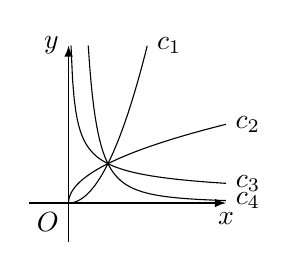
\begin{tikzpicture}[>=latex,scale = 0.5]
        \draw [->] (-1,0) -- (4,0) node [below] {$x$};
        \draw [->] (0,-1) -- (0,4) node [left] {$y$};
        \draw (0,0) node [below left] {$O$};
        \draw [domain = 0:2, samples = 100] plot (\x,\x*\x) node [right] {$c_1$};
        \draw [domain = 0:2, samples = 100] plot (\x*\x,\x) node [right] {$c_2$};
        \draw [domain = 0.0625:4, samples = 100] plot (\x, {1/sqrt(\x)}) node [right] {$c_3$};
        \draw [domain = 0.5:4, samples = 100] plot (\x, {1/\x/\x}) node [right] {$c_4$};
    \end{tikzpicture}
    \end{center}
\fourch{$-2,-\dfrac 12,\dfrac 12,2$}{$2,\dfrac 12,-\dfrac 12,-2$
}{$-\dfrac 12,-2,2,\dfrac 12$}{$2,\dfrac 12,-2,-\dfrac 12$}


关联目标:

K0207003B|D02002B|会根据函数定义域, 利用计算器合理采点, 并能通过描点法作出幂函数$y=x^{1/2}$,$y=x^{3}$,$y=x^{-2/3}$的大致图像.



标签: 第二单元

答案: 暂无答案

解答或提示: 暂无解答与提示

使用记录:

暂无使用记录


出处: 2022届高三第一轮复习讲义
\item { (002910)}下列函数的图像为(A)、(B)、(C)、(D)之一, 试将正确的字母标号填在相应函数后面的横线上.
\begin{center}
    \begin{tikzpicture}[>=latex,scale = 0.5]
        \draw [->] (-3,0) -- (3,0) node [below] {$x$};
        \draw [->] (0,-3) -- (0,3) node [left] {$y$};
        \draw (0,0) node [below right] {$O$};
        \draw [domain = {-3^(1/4)}:{3^(1/4)}] plot (\x*\x*\x,\x*\x*\x*\x);
        \draw (0,-3) node [below] {(A)};
    \end{tikzpicture}
    \begin{tikzpicture}[>=latex,scale = 0.5]
        \draw [->] (-3,0) -- (3,0) node [below] {$x$};
        \draw [->] (0,-3) -- (0,3) node [left] {$y$};
        \draw (0,0) node [below right] {$O$};
        \draw [domain = {-3^(1/5)}:{3^(1/5)}] plot (\x*\x*\x,\x*\x*\x*\x*\x);
        \draw (0,-3) node [below] {(B)};
    \end{tikzpicture}
    \begin{tikzpicture}[>=latex,scale =0.5]
        \draw [->] (-3,0) -- (3,0) node [below] {$x$};
        \draw [->] (0,-3) -- (0,3) node [left] {$y$};
        \draw (0,0) node [below right] {$O$};
        \draw [domain = {0}:{3^(1/3)}] plot (\x*\x,\x*\x*\x);
        \draw (0,-3) node [below] {(C)};
    \end{tikzpicture}
    \begin{tikzpicture}[>=latex,scale = 0.5]
        \draw [->] (-3,0) -- (3,0) node [below] {$x$};
        \draw [->] (0,-3) -- (0,3) node [left] {$y$};
        \draw (0,0) node [below right] {$O$};
        \draw [domain = {3^(-3/2)}:3] plot (\x,{\x^(-2/3)}) plot (-\x,{\x^(-2/3)});
        \draw (0,-3) node [below] {(D)};
    \end{tikzpicture}
    \end{center}
(1) $y=x^\frac 32$\blank{50}; (2) $y=x^\frac 43$\blank{50}; (3) $y=x^\frac 53$\blank{50}; (4) $y=x^{-\frac 23}$\blank{50}.


关联目标:

暂未关联目标



标签: 第二单元

答案: 暂无答案

解答或提示: 暂无解答与提示

使用记录:

暂无使用记录


出处: 2022届高三第一轮复习讲义
\item { (002915)}设常数$n\in \mathbf{Z}$. 若函数$y=x^{n^2-2n-3}$的图像与两条坐标轴都无公共点, 且图像关于$y$轴对称, 则$n$的值为\blank{50}.


关联目标:

暂未关联目标



标签: 第二单元

答案: 暂无答案

解答或提示: 暂无解答与提示

使用记录:

暂无使用记录


出处: 2022届高三第一轮复习讲义
\item { (002916)}函数$y=1-(x+2)^{-2}$可以先将幂函数$y=x^{-2}$的图像向\blank{50}平移$2$个单位, 再以\blank{50}轴为对称轴作对称变换, 最后向\blank{50}平移$1$个单位.


关联目标:

暂未关联目标



标签: 第二单元

答案: 暂无答案

解答或提示: 暂无解答与提示

使用记录:

暂无使用记录


出处: 2022届高三第一轮复习讲义
\item { (002917)}在$f(x)=(2m^2-7m-9)x^{m^2-9m+19}$中, 当实数$m$为何值时,\\
(1) $y=f(x)$是正比例函数, 且它的图像的倾斜角为钝角?\\
(2) $y=f(x)$是反比例函数, 且它的图像在第一, 三象限?


关联目标:

暂未关联目标



标签: 第二单元

答案: 暂无答案

解答或提示: 暂无解答与提示

使用记录:

暂无使用记录


出处: 2022届高三第一轮复习讲义
\item { (002918)}设常数$t\in \mathbf{Z}$. 已知幂函数$y=(t^3-t+1){x^{\frac 13(1+2t-t^2)}}$是偶函数, 且在区间$(0,+\infty)$上是增函数, 求整数$t$的值, 并作出相应的幂函数的大致图像.


关联目标:

K0207004B|D02002B|会用图像上任意一点关于原点(或关于$y$轴)的对称点仍落在图像上证明函数的图像关于原点(或$y$轴)对称.

K0208002B|D02002B|会经历作图猜想证明具体的幂函数图像在第一象限的单调性.



标签: 第二单元

答案: 暂无答案

解答或提示: 暂无解答与提示

使用记录:

暂无使用记录


出处: 2022届高三第一轮复习讲义
\item { (002920)}已知函数: \textcircled{1} $y=\dfrac 1x$; \textcircled{2} $y=x^{\dfrac 12}$; \textcircled{3} $y=x^{-\dfrac 12}$; \textcircled{4} $y={x^{\dfrac 23}}$; \textcircled{5} $y=x^{-\dfrac 23}$, 填写分别具有下列性质的函数序号:\\ 
(1) 图像与$x$轴有公共点的:\blank{50};\\
(2) 图像关于原点对称的:\blank{50};\\
(3) 定义域内递减的:\blank{50};\\
(4) 在定义域内有反函数的:\blank{50}.


关联目标:

暂未关联目标



标签: 第二单元

答案: 暂无答案

解答或提示: 暂无解答与提示

使用记录:

暂无使用记录


出处: 2022届高三第一轮复习讲义
\item { (002921)}函数$y=-(x+1)^{-3}$的图像可以先将幂函数$y=x^{-3}$的图像向\blank{50}平移1个单位, 再以\blank{50}轴为对称轴作对称变换.


关联目标:

暂未关联目标



标签: 第二单元

答案: 暂无答案

解答或提示: 暂无解答与提示

使用记录:

暂无使用记录


出处: 2022届高三第一轮复习讲义
\item { (002923)}下列关于幂函数图像及性质的叙述中, 正确的叙述的序号是\blank{50}.\\
\textcircled{1} 对于一个确定的幂函数, 第二、三象限不可能同时有该幂函数的图像上的点;\\
\textcircled{2} 若某个幂函数图像过$(-1,-1)$, 则该幂函数是奇函数;\\
\textcircled{3} 若某个幂函数在定义域上递增, 则该幂函数图像必经过原点;\\
\textcircled{4} 幂函数图像不会经过点$(-\dfrac 12,8)$以及$(-8,-4)$.


关联目标:

暂未关联目标



标签: 第二单元

答案: 暂无答案

解答或提示: 暂无解答与提示

使用记录:

暂无使用记录


出处: 2022届高三第一轮复习讲义
\item { (002925)}已知幂函数$y=x^{\frac qp}$($p\in \mathbf{N}^*,\ q\in \mathbf{N}^*$, $p,q$互质)的图像如图所示, 则\bracket{20}.
\begin{center}
    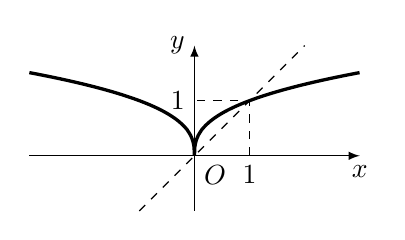
\begin{tikzpicture}[>=latex,scale = 0.7]
        \draw [->] (-3,0) -- (3,0) node [below] {$x$};
        \draw [->] (0,-1) -- (0,2) node [left] {$y$};
        \draw (0,0) node [below right] {$O$};
        \draw [dashed] (-1,-1) -- (2,2);
        \draw [domain = 0:3, samples = 400, very thick] plot (\x,{\x^(3/8)}) plot (-\x,{\x^(3/8)});
        \draw [dashed] (1,0) node [below] {$1$} -- (1,1) -- (0,1) node [left] {$1$};
    \end{tikzpicture}
\end{center}
\twoch{$p,q$均为奇数}{$p$是奇数, $q$是偶数, 且$0<\dfrac qp<1$}{$p$是偶数, $q$是奇数}{$p$是奇数, $q$是偶数, 且$\dfrac qp>1$}


关联目标:

K0207003B|D02002B|会根据函数定义域, 利用计算器合理采点, 并能通过描点法作出幂函数$y=x^{1/2}$,$y=x^{3}$,$y=x^{-2/3}$的大致图像.

K0207004B|D02002B|会用图像上任意一点关于原点(或关于$y$轴)的对称点仍落在图像上证明函数的图像关于原点(或$y$轴)对称.



标签: 第二单元

答案: 暂无答案

解答或提示: 暂无解答与提示

使用记录:

暂无使用记录


出处: 2022届高三第一轮复习讲义
\item { (002927)}设常数$a,b$满足$a>b>0$. 已知函数$f(x)=\dfrac{x+a}{x+b}$.
(1) 写出函数$y=f(x)$的单调性;\\
(2) 写出函数$y=f(x)$图像的一个对称中心的坐标.


关联目标:

暂未关联目标



标签: 第二单元

答案: 暂无答案

解答或提示: 暂无解答与提示

使用记录:

暂无使用记录


出处: 2022届高三第一轮复习讲义
\item { (002929)}*设常数$a,b$满足$a>b>0$. 已知函数$f(x)=\dfrac{x+a}{x+b}$. 证明: 该函数图像的对称中心是唯一的.


关联目标:

暂未关联目标



标签: 第二单元

答案: 暂无答案

解答或提示: 暂无解答与提示

使用记录:

暂无使用记录


出处: 2022届高三第一轮复习讲义
\item { (002936)}若函数$f(x)=1-\sqrt{1-x^2}\ (-1\le x\le 0)$,
请画出函数$y={f^{-1}}(x)$的大致图像.
\begin{center}
    \begin{tikzpicture}[>=latex,scale =1.8]
        \foreach \i in {-1,-0.5,0,0.5,1} {\draw [dashed, gray!90] (\i,-1) -- (\i,1) (-1,\i) -- (1,\i);};
        \draw [->] (-1.5,0) -- (1.5,0) node [below] {$x$};
        \draw [->] (0,-1.5) -- (0,1.5) node [left] {$y$};
        \draw (0,0) node [below left] {$O$};
        \draw (1,0) node [below] {$1$} (0,1) node [left] {$1$};
    \end{tikzpicture}
\end{center}


关联目标:

暂未关联目标



标签: 第二单元

答案: 暂无答案

解答或提示: 暂无解答与提示

使用记录:

暂无使用记录


出处: 2022届高三第一轮复习讲义
\item { (002937)}已知定义在$\mathbf{R}$上的函数$y=f(x)$是奇函数, 且有反函数$y=f^{-1}(x)$. 若$a,b$是两个实数, 则下列点中, 必在$y=f^{-1}(x)$的图像上的点的序号是\blank{50}.\\
\textcircled{1} $(-f(a),a)$; \textcircled{2} $(-f(a),-a)$;\textcircled{3} $(-b,-f(b))$; \textcircled{4} $(b,-f^{-1}(-b))$.


关联目标:

暂未关联目标



标签: 第二单元

答案: 暂无答案

解答或提示: 暂无解答与提示

使用记录:

暂无使用记录


出处: 2022届高三第一轮复习讲义
\item { (002938)}已知定义在$\mathbf{R}$上的函数$y=f(x)$的反函数为$y=f^{-1}(x)$.若$y=f(x+1)$的图像过点$(-\dfrac 12,1)$, 则$y=f^{-1}(x+1)$的图像必过\bracket{20}.
\fourch{$(1,-\dfrac 12)$}{$(1,\dfrac 12)$}{$(0,-\dfrac 12)$}{$(0,\dfrac 12)$}


关联目标:

暂未关联目标



标签: 第二单元

答案: 暂无答案

解答或提示: 暂无解答与提示

使用记录:

暂无使用记录


出处: 2022届高三第一轮复习讲义
\item { (002939)}设常数$a\ne 0$. 若函数$f(x)=\dfrac{1-ax}{1+ax}$的图像关于直线$y=x$对称, 求实数$a$的值以及$y=f(x)$的反函数$y=f^{-1}(x)$.


关联目标:

暂未关联目标



标签: 第二单元

答案: 暂无答案

解答或提示: 暂无解答与提示

使用记录:

暂无使用记录


出处: 2022届高三第一轮复习讲义
\item { (002940)}记$y=f^{-1}(x)$是$y=f(x)$的反函数.\\
(1) 若函数$f(x+1)=\dfrac x{x+1}$, 求函数$y=f^{-1}(x+1)$的解析式;\\
(2) 设函数$f(x)=\dfrac{1-2x}{1+x}$. 若$y=g(x)$的图像与$y=f^{-1}(x+1)$的图像关于直线$y=x$对称, 求$y=g(x)$的解析式.


关联目标:

暂未关联目标



标签: 第二单元

答案: 暂无答案

解答或提示: 暂无解答与提示

使用记录:

暂无使用记录


出处: 2022届高三第一轮复习讲义
\item { (002946)}已知函数$y=f(x)$的图像经过点$(0,-1)$. 若函数$y=f(x+4)$存在反函数$y=g(x)$, 则$y=g(x)$的图像总经过的定点的坐标为\blank{50}.


关联目标:

暂未关联目标



标签: 第二单元

答案: 暂无答案

解答或提示: 暂无解答与提示

使用记录:

暂无使用记录


出处: 2022届高三第一轮复习讲义
\item { (002947)}设$y=f^{-1}(x)$, $y=g^{-1}(x)$分别是定义在$\mathbf{R}$上的函数$y=f(x)$, $y=g(x)$的反函数. 若函数$y=f(x-1)$和$y=g^{-1}(x-3)$的图像关于直线$y=x$对称, 且$g(5)=2018$, 则 $f(4)$的值为\blank{50}.


关联目标:

暂未关联目标



标签: 第二单元

答案: 暂无答案

解答或提示: 暂无解答与提示

使用记录:

暂无使用记录


出处: 2022届高三第一轮复习讲义
\item { (002953)}函数$f(x)=\dfrac{\sqrt{4-x^2}}{\lg |x-1|}$的定义域为\blank{50}.


关联目标:

暂未关联目标



标签: 第二单元

答案: 暂无答案

解答或提示: 暂无解答与提示

使用记录:

暂无使用记录


出处: 2022届高三第一轮复习讲义
\item { (002954)}为了得到函数$y=\lg\dfrac{x+3}{10}$的图像, 只需把函数$y=\lg x$的图像上所有的点\bracket{20}.
\onech{向左平移$3$个单位长度, 再向上平移$1$个单位长度}{向右平移$3$个单位长度, 再向上平移$1$个单位长度}{向左平移$3$个单位长度, 再向下平移$1$个单位长度}{向右平移$3$个单位长度, 再向下平移$1$个单位长度}


关联目标:

暂未关联目标



标签: 第二单元

答案: 暂无答案

解答或提示: 暂无解答与提示

使用记录:

暂无使用记录


出处: 2022届高三第一轮复习讲义
\item { (002958)}已知函数$f(x)=\dfrac{3^x-3^{-x}}{3^x+3^{-x}}$.\\
(1) 证明$f(x)$在$(-\infty,+\infty)$上是增函数;\\
(2) 求$f(x)$的值域.


关联目标:

暂未关联目标



标签: 第二单元

答案: 暂无答案

解答或提示: 暂无解答与提示

使用记录:

暂无使用记录


出处: 2022届高三第一轮复习讲义
\item { (002964)}对于函数$y=f(x)$的定义域中的任意的$x_1,x_2$($x_1\ne x_2$), 有如下结论:\\
\textcircled{1} $f(x_1+x_2)=f(x_1)\cdot f(x_2)$; \textcircled{2} $f(x_1\cdot x_2)=f(x_1)+f(x_2)$;\\ \textcircled{3} $\dfrac{f(x_1)-f(x_2)}x_1-x_2>0$; \textcircled{4} $f(\dfrac{x_1+x_2}2)<\dfrac{f(x_1)+f(x_2)}2$. 
\\当$y=\ln x$时, 上述结论中, 正确结论的序号是\blank{50}.


关联目标:

暂未关联目标



标签: 第二单元

答案: 暂无答案

解答或提示: 暂无解答与提示

使用记录:

暂无使用记录


出处: 2022届高三第一轮复习讲义
\item { (002966)}*已知常数$a>1$, 函数$y=|\log_ax|$的定义域为区间$[m,n]$, 值域为区间$[0,1]$. 若$n-m$的最小值为$\dfrac 56$, 则$a$=\blank{50}.


关联目标:

暂未关联目标



标签: 第二单元

答案: 暂无答案

解答或提示: 暂无解答与提示

使用记录:

暂无使用记录


出处: 2022届高三第一轮复习讲义
\item { (002968)}*已知函数$f(x)=2+\log_3 x\ (3\le x\le 27)$.\\
(1) 求函数$y=f(x^2)$的定义域;\\
(2) 求函数$g(x)={[f(x)]}^2+f(x^2)$的值域.


关联目标:

暂未关联目标



标签: 第二单元

答案: 暂无答案

解答或提示: 暂无解答与提示

使用记录:

暂无使用记录


出处: 2022届高三第一轮复习讲义
\item { (002969)}已知定义域为$\mathbf{R}$的函数$y=f(x)$为奇函数, 且满足$f(x+2)=-f(x)$. 当$x\in [0,1]$时, $f(x)=2^x-1$.\\
(1) 求$y=f(x)$在区间$[-1,0)$上的解析式;\\
(2) 求$f(\log_{\frac 12}24)$的值.


关联目标:

暂未关联目标



标签: 第二单元

答案: 暂无答案

解答或提示: 暂无解答与提示

使用记录:

暂无使用记录


出处: 2022届高三第一轮复习讲义
\item { (002970)}*已知函数$f(x)=1+a\cdot (\dfrac 12)^x+(\dfrac 14)^x$.\\
(1) 当$a=1$时, 求函数$y=f(x)$在$(-\infty,0)$上的值域;\\
(2) 对于定义在集合$D$上的函数$y=f(x)$, 如果存在常数$M>0$, 满足: 对任意$x\in D$, 都有$|f(x)|\le M$成立, 则称$f(x)$是$D$上的有界函数, 其中$M$称为函数$f(x)$的一个上界.若函数$y=f(x)$在$[0,+\infty)$上是以$3$为一个上界的有界函数, 求实数$a$的取值范围.


关联目标:

暂未关联目标



标签: 第二单元

答案: 暂无答案

解答或提示: 暂无解答与提示

使用记录:

暂无使用记录


出处: 2022届高三第一轮复习讲义
\item { (002971)}二次函数图像的顶点是$(-1,2)$, 且图像经过点$(1,6)$, 则此二次函数的解析式为\blank{50}.


关联目标:

暂未关联目标



标签: 第二单元

答案: 暂无答案

解答或提示: 暂无解答与提示

使用记录:

暂无使用记录


出处: 2022届高三第一轮复习讲义
\item { (002972)}二次函数$y=f(x)$满足$f(2-x)=f(2+x)$, 且$y=f(x)$的图像在$y$轴的截距为$3$, 被$x$轴截得的线段长为$2$, 则$y=f(x)$的解析式为\blank{50}.


关联目标:

暂未关联目标



标签: 第二单元

答案: 暂无答案

解答或提示: 暂无解答与提示

使用记录:

暂无使用记录


出处: 2022届高三第一轮复习讲义
\item { (002985)}函数$f(x)=\dfrac 12x^2-x+\dfrac 32$的定义域、值域都是区间$[1,b]$, 则实数$b$=\blank{50}.


关联目标:

暂未关联目标



标签: 第二单元

答案: 暂无答案

解答或提示: 暂无解答与提示

使用记录:

暂无使用记录


出处: 2022届高三第一轮复习讲义
\item { (002986)}设常数$m\in \mathbf{R}$. 若函数$f(x)=x^2-(m-2)x+m-4$的图像与x轴交于$A$, $B$两点, 且$|AB|=2$, 则函数$y=f(x)$的最小值为\blank{50}.


关联目标:

暂未关联目标



标签: 第二单元

答案: 暂无答案

解答或提示: 暂无解答与提示

使用记录:

暂无使用记录


出处: 2022届高三第一轮复习讲义
\item { (002987)}函数$f(x)=ax^2+bx+c$ 与函数$g(x)=cx^2+bx+a$($ac\ne 0,\ a\ne c)$的值域分别为$M$、$N$, 则下列结论正确的是\blank{50}.
\fourch{$M=N$}{$M\subseteq N$}{$M\supseteq N$}{$M\cap N\ne \varnothing$}


关联目标:

暂未关联目标



标签: 第二单元

答案: 暂无答案

解答或提示: 暂无解答与提示

使用记录:

暂无使用记录


出处: 2022届高三第一轮复习讲义
\item { (002988)}函数$f(x)=x^2-2a|x-a|-2ax+1$的图像与$x$轴有且只有三个不同的公共点, 则$a=$\blank{50}.


关联目标:

暂未关联目标



标签: 第二单元

答案: 暂无答案

解答或提示: 暂无解答与提示

使用记录:

暂无使用记录


出处: 2022届高三第一轮复习讲义
\item { (002990)}设常数$a,m\in \mathbf{R}$. 已知函数$f(x)=\dfrac{x^2+2x+a}x\  (x\ge m)$.\\
(1) 设$a=\dfrac 12$, 求函数$y=f(x)$的值域;\\
(2) 设$m=1$, 求函数$y=f(x)$的值域.


关联目标:

暂未关联目标



标签: 第二单元

答案: 暂无答案

解答或提示: 暂无解答与提示

使用记录:

暂无使用记录


出处: 2022届高三第一轮复习讲义
\item { (002993)}函数$y=\dfrac{3^x-1}{3^x-2}$的值域是\blank{50}.


关联目标:

暂未关联目标



标签: 第二单元

答案: 暂无答案

解答或提示: 暂无解答与提示

使用记录:

暂无使用记录


出处: 2022届高三第一轮复习讲义
\item { (002994)}函数$y=\log_{\frac 12}(-x^2+2x+3)$的值域是\blank{50}.


关联目标:

暂未关联目标



标签: 第二单元

答案: 暂无答案

解答或提示: 暂无解答与提示

使用记录:

暂无使用记录


出处: 2022届高三第一轮复习讲义
\item { (002995)}函数$y=|x-1|+|x-3|$的值域是\blank{50}.


关联目标:

暂未关联目标



标签: 第二单元

答案: 暂无答案

解答或提示: 暂无解答与提示

使用记录:

暂无使用记录


出处: 2022届高三第一轮复习讲义
\item { (002996)}(1) 函数$y=x^2+\dfrac 8{x^2+1}$($1\le x\le 7$)的最小值是\blank{50}, 此时$x$=\blank{50};\\
(2) 函数$y=\dfrac{3x}{x^2+4}$的值域是\blank{50};\\
(3) 函数$y=x+\dfrac m{x+3}$ , $x\in [0,+\infty)$的最小值为\blank{50};\\
(4) 设常数$m\in \mathbf{R}$. 若函数$y=\dfrac{mx}{x^2+1}$的最大值为$1$, 则$m$的值为\blank{50}.


关联目标:

暂未关联目标



标签: 第二单元

答案: 暂无答案

解答或提示: 暂无解答与提示

使用记录:

暂无使用记录


出处: 2022届高三第一轮复习讲义
\item { (002997)}(1) 函数$y=x-\sqrt{1-2x}$的最大值为\blank{50}, 此时$x$=\blank{50};\\
(2) 函数$y=2x+\sqrt{1-2x}$的值域是\blank{50}.


关联目标:

暂未关联目标



标签: 第二单元

答案: 暂无答案

解答或提示: 暂无解答与提示

使用记录:

暂无使用记录


出处: 2022届高三第一轮复习讲义
\item { (002998)}函数$y=\dfrac{2x-3}{x^2-2x+3}$的值域是\blank{50}.


关联目标:

暂未关联目标



标签: 第二单元

答案: 暂无答案

解答或提示: 暂无解答与提示

使用记录:

暂无使用记录


出处: 2022届高三第一轮复习讲义
\item { (003000)}已知函数$f(x)=\log_a(x+\sqrt{x^2+1}), \ a>1$.\\
(1) 求$f(x)$的定义域和值域;\\
(2) 求$f^{-1}(x)$;\\
(3) 判断$f^{-1}(x)$的奇偶性、单调性;\\
(4) 若实数$m$满足$f^{-1}(1-m)+f^{-1}(1-m^2)<0$, 求$m$的范围.


关联目标:

暂未关联目标



标签: 第二单元

答案: 暂无答案

解答或提示: 暂无解答与提示

使用记录:

暂无使用记录


出处: 2022届高三第一轮复习讲义
\item { (003001)}*设常数$m,n\in \mathbf{R}$. 若函数$y=\dfrac{mx^2+4x+n}{x^2+1}$的值域为$[1,6]$, 求$m,n$的值.


关联目标:

暂未关联目标



标签: 第二单元

答案: 暂无答案

解答或提示: 暂无解答与提示

使用记录:

暂无使用记录


出处: 2022届高三第一轮复习讲义
\item { (003002)}设常数$a\in \mathbf{R}$, 区间$E\subseteq (0,+\infty)$. 已知函数$f(x)=\dfrac 1a-\dfrac 1x$, $x\in E$.\\
(1) 求证: $y=f(x)$在区间$E$上递增;\\
(2) 是否存在$a$, 使得对于这样的$a$, 总是存在 $E=[m,n]$($m<n$), 使得$y=f(x)$在区间$E$上的值域也是$E$? 若存在, 求出$a$的取值范围; 若不存在, 说明理由.


关联目标:

暂未关联目标



标签: 第二单元

答案: 暂无答案

解答或提示: 暂无解答与提示

使用记录:

暂无使用记录


出处: 2022届高三第一轮复习讲义
\item { (003003)}函数$y=2x+\dfrac 4x$($\dfrac 12<x\le 2$)的值域是\blank{50}.


关联目标:

暂未关联目标



标签: 第二单元

答案: 暂无答案

解答或提示: 暂无解答与提示

使用记录:

暂无使用记录


出处: 2022届高三第一轮复习讲义
\item { (003004)}函数$y=|x-3|-|x+2|$的值域是\blank{50}.


关联目标:

暂未关联目标



标签: 第二单元

答案: 暂无答案

解答或提示: 暂无解答与提示

使用记录:

暂无使用记录


出处: 2022届高三第一轮复习讲义
\item { (003005)}函数$y=(\dfrac 12)^{x^2-x}$的值域是\blank{50}.


关联目标:

暂未关联目标



标签: 第二单元

答案: 暂无答案

解答或提示: 暂无解答与提示

使用记录:

暂无使用记录


出处: 2022届高三第一轮复习讲义
\item { (003006)}函数$y=\dfrac{\sqrt x}{x+1}$的值域是\blank{50}.


关联目标:

暂未关联目标



标签: 第二单元

答案: 暂无答案

解答或提示: 暂无解答与提示

使用记录:

暂无使用记录


出处: 2022届高三第一轮复习讲义
\item { (003009)}求函数$y=\dfrac{2x^2-4x-1}{x^2-2x-1}$的值域.


关联目标:

暂未关联目标



标签: 第二单元

答案: 暂无答案

解答或提示: 暂无解答与提示

使用记录:

暂无使用记录


出处: 2022届高三第一轮复习讲义
\item { (003010)}求函数$y=\dfrac{x^2+4x-1}{x^2-2x+1}$($2\le x\le 3$)的值域.


关联目标:

暂未关联目标



标签: 第二单元

答案: 暂无答案

解答或提示: 暂无解答与提示

使用记录:

暂无使用记录


出处: 2022届高三第一轮复习讲义
\item { (003011)}记$\max\{a_1,a_2,\cdots,a_n\}$为$a_1,\cdots,a_n$中的最大值. 已知$f(x)=\max\{x,x^2\}$($-1\le x\le 3$).\\
(1) 求函数$y=f(x)$的值域;\\
(2) 设$PAB$三点的坐标分别为$(x,f(x))$, $(0,-1)$, $(2,0)$, 且$PAB$三点可以构成三角形, 求$\triangle PAB$的面积的取值范围.


关联目标:

暂未关联目标



标签: 第二单元

答案: 暂无答案

解答或提示: 暂无解答与提示

使用记录:

暂无使用记录


出处: 2022届高三第一轮复习讲义
\item { (003012)}是否存在实数$m,n$($m<n$), 使得函数$f(x)=-x^2+2$的定义域、值域分别是区间$[m,n]$、$[2m,2n]$. 若存在, 求出$m,n$的值; 若不存在, 说明理由.


关联目标:

暂未关联目标



标签: 第二单元

答案: 暂无答案

解答或提示: 暂无解答与提示

使用记录:

暂无使用记录


出处: 2022届高三第一轮复习讲义
\item { (003620)}已知$a\in \mathbf{R}$, 若存在定义域为$\mathbf{R}$的函数$f(x)$同时满足下列两个条件, \textcircled{1} 对任意$x_0\in \mathbf{R}$, $f(x_0)$的值为$x_0$或$x_0^2$; \textcircled{2} 关于$x$的方程$f(x)=a$无实数解; 则$a$的取值范围为\blank{50}.


关联目标:

暂未关联目标



标签: 第二单元

答案: 暂无答案

解答或提示: 暂无解答与提示

使用记录:

20220630	2022届高三1班	\fcolorbox[rgb]{0,0,0}{1.000,0.326,0}{0.837}


出处: 上海2020年秋季高考试题11
\item { (003642)}已知$f(x)=\left|\dfrac{2}{x-1}-a\right| \ (x>1, \ a>0)$, $f(x)$的图像与$x$轴的交点为$A$, 若对于$f(x)$的图像上任意一点$P$, 在其图像上总存在另一点$Q$($P$、$Q$异于$A$), 满足$AP\perp AQ$, 且$|AP|=|AQ|$, 则$a=$\blank{50}.


关联目标:

暂未关联目标



标签: 第二单元

答案: 暂无答案

解答或提示: 暂无解答与提示

使用记录:

20220630	2022届高三1班	\fcolorbox[rgb]{0,0,0}{1.000,0.466,0}{0.767}


出处: 上海2019年秋季高考试题12
\item { (003655)}设常数$a\in \mathbf{R}$, 函数$f(x)=\log_2(x+a)$. 若$f(x)$的反函数的图像经过点$(3,1)$, 则$a=$\blank{50}.


关联目标:

暂未关联目标



标签: 第二单元

答案: 暂无答案

解答或提示: 暂无解答与提示

使用记录:

暂无使用记录


出处: 上海2018年秋季高考试题4
\item { (003662)}已知常数$a>0$, 函数$f(x)=\dfrac{2^x}{2^x+ax}$的图像经过点$P\left(p,\dfrac{6}{5}\right)$, $Q\left(q,-\dfrac{1}{5}\right)$. 若$2^{p+q}=36pq$, 则$a=$\blank{50}.


关联目标:

K0203005B|D02001B|会应用底数为正实数的实数指数幂的定义、运算性质以及幂的基本不等式, 解决底数为正实数的实数指数幂的较复杂的表达式的化简、不等式的证明等问题.



标签: 第二单元

答案: 暂无答案

解答或提示: 暂无解答与提示

使用记录:

20220630	2022届高三1班	\fcolorbox[rgb]{0,0,0}{1.000,0.000,0}{1.000}


出处: 上海2018年秋季高考试题11
\item { (003667)}设$D$是含数$1$的有限实数集, $f(x)$是定义在$D$上的函数. 若$f(x)$的图像绕原点逆时针旋转$\dfrac{\pi}{6}$后与原图像重合, 则在以下各项中, $f(1)$的可能取值只能是\bracket{15}.
\fourch{$\sqrt{3}$}{$\dfrac{\sqrt{3}}{2}$}{$\dfrac{\sqrt{3}}{3}$}{$0$}


关联目标:

暂未关联目标



标签: 第二单元

答案: 暂无答案

解答或提示: 暂无解答与提示

使用记录:

20220630	2022届高三1班	\fcolorbox[rgb]{0,0,0}{1.000,0.140,0}{0.930}


出处: 上海2018年秋季高考试题16
\item { (003681)}已知四个函数: \textcircled{1} $y=-x$, \textcircled{2} $y=-\dfrac{1}{x}$, \textcircled{3} $y=x^3$, \textcircled{4} $y=x^{\frac{1}{2}}$. 从中任选$2$个, 则事件``所选$2$个函数的图像有且仅有一个公共点''的概率为\blank{50}.


关联目标:

暂未关联目标



标签: 第二单元

答案: 暂无答案

解答或提示: 暂无解答与提示

使用记录:

暂无使用记录


出处: 上海2017年秋季高考试题9
\item { (003709)}若函数$y=a^x+b$($a>0$且$a\ne 1$)的图像经过点$(1,7)$, 其反函数的图像经过点$(4,0)$, 则$a-b=$\blank{50}.


关联目标:

暂未关联目标



标签: 第二单元

答案: 暂无答案

解答或提示: 暂无解答与提示

使用记录:

暂无使用记录


出处: 2016年双基百分百
\item { (003720)}函数$y=\sqrt{2016^{1-x}}$的定义域是\blank{50}.


关联目标:

暂未关联目标



标签: 第二单元

答案: 暂无答案

解答或提示: 暂无解答与提示

使用记录:

暂无使用记录


出处: 2016年双基百分百
\item { (003726)}若函数$f(x)=\dfrac{k-2^x}{1+k\cdot 2^x}, \ (k\ne 1, \ k\in \mathbf{R})$在定义域内为奇函数, 则$k=$\blank{50}.


关联目标:

暂未关联目标



标签: 第二单元

答案: 暂无答案

解答或提示: 暂无解答与提示

使用记录:

暂无使用记录


出处: 2016年双基百分百
\item { (003730)}下列函数中, 与函数$y=x^{2n+1} \ (n\in \mathbf{N}^*)$的值域相同的函数为\blank{30}.
\fourch{$y=\left(\dfrac 12\right)^{x+1}$}{$y=\ln(x+1)$}{$y=\dfrac{x+1}{x}$}{$y=x+\dfrac 1x$}


关联目标:

暂未关联目标



标签: 第二单元

答案: 暂无答案

解答或提示: 暂无解答与提示

使用记录:

暂无使用记录


出处: 2016年双基百分百
\item { (003732)}函数$f(x)=\sqrt{27-3^{2x+1}}$的定义域是\blank{50}.(用区间表示)


关联目标:

暂未关联目标



标签: 第二单元

答案: 暂无答案

解答或提示: 暂无解答与提示

使用记录:

暂无使用记录


出处: 2016年双基百分百
\item { (003746)}幂函数$f(x)$的图像经过点$(2,\sqrt{2})$, 且$f^{-1}(x)$为$f(x)$的反函数, 则$f^{-1}(4)=$\blank{50}.


关联目标:

暂未关联目标



标签: 第二单元

答案: 暂无答案

解答或提示: 暂无解答与提示

使用记录:

暂无使用记录


出处: 2016年双基百分百
\item { (003783)}(理科)已知$f(x)$是$\mathbf{R}$上的奇函数, $g(x)$是$\mathbf{R}$上的偶函数, 若函数$f(x)+g(x)$的值域为$[1,3)$, 则$f(x)-g(x)$的值域为\blank{50}.\\
(文科)已知$f(x)$是$\mathbf{R}$上的奇函数, $g(x)$是$\mathbf{R}$上的偶函数, 若函数$f(x)+g(x)$的值域为$[1,3)$, 则$f(-x)+g(x)$的值域为\blank{50}.


关联目标:

暂未关联目标



标签: 第二单元

答案: 暂无答案

解答或提示: 暂无解答与提示

使用记录:

暂无使用记录


出处: 2016年双基百分百
\item { (003789)}设函数$f(x)=\log_\frac 12 x$, $g(x)=f^{-1}(|x|)$.\\
(1) 求函数$g(x)$的解析式, 并画出大致图像;\\
(2) 若不等式$g(x)+g(2x)\le k$对任意$x\in \mathbf{R}$恒成立, 求实数$k$的取值范围.


关联目标:

暂未关联目标



标签: 第二单元

答案: 暂无答案

解答或提示: 暂无解答与提示

使用记录:

暂无使用记录


出处: 2016年双基百分百
\item { (003815)}在同一坐标系中画出函数$y=\log_a x, \ y=a^x, y=x+a$的图像, 可能正确的是\blank{30}.
\fourch{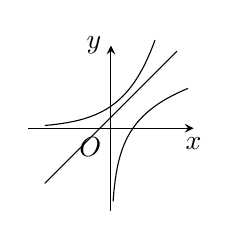
\begin{tikzpicture}[>=stealth,samples=100, scale = 0.7]
\draw [->] (-1.5,0)--(0,0) node [below left] {$O$}--(1.5,0) node [below] {$x$};
\draw [->] (0,-1.5)--(0,1.5) node [left] {$y$};
\draw [domain=-3:3] plot ({\x*0.4},{(\x+0.5)*0.4});
\draw [domain=-3:2] plot ({\x*0.4},{exp(\x*ln(2))*0.4});
\draw [domain=0.1:3.5] plot ({\x*0.4},{ln(\x)/ln(2)*0.4});
\end{tikzpicture}}{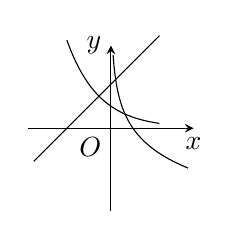
\begin{tikzpicture}[>=stealth,samples=100, scale = 0.7]
\draw [->] (-1.5,0)--(0,0) node [below left] {$O$}--(1.5,0) node [below] {$x$};
\draw [->] (0,-1.5)--(0,1.5) node [left] {$y$};
\draw [domain=-3.5:2.2] plot ({\x*0.4},{(\x+2)*0.4});
\draw [domain=-2:2.2] plot ({\x*0.4},{exp(\x*ln(1/2))*0.4});
\draw [domain=0.1:3.5] plot ({\x*0.4},{-ln(\x)/ln(2)*0.4});
\end{tikzpicture}}{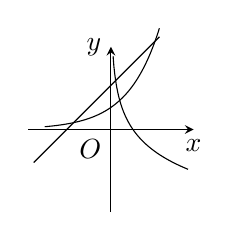
\begin{tikzpicture}[>=stealth,samples=100, scale = 0.7]
\draw [->] (-1.5,0)--(0,0) node [below left] {$O$}--(1.5,0) node [below] {$x$};
\draw [->] (0,-1.5)--(0,1.5) node [left] {$y$};
\draw [domain=-3.5:2.2] plot ({\x*0.4},{(\x+2)*0.4});
\draw [domain=-3:2.2] plot ({\x*0.4},{exp(\x*ln(2))*0.4});
\draw [domain=0.1:3.5] plot ({\x*0.4},{-ln(\x)/ln(2)*0.4});
\end{tikzpicture}}{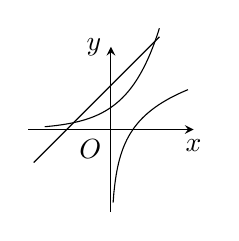
\begin{tikzpicture}[>=stealth,samples=100, scale = 0.7]
\draw [->] (-1.5,0)--(0,0) node [below left] {$O$}--(1.5,0) node [below] {$x$};
\draw [->] (0,-1.5)--(0,1.5) node [left] {$y$};
\draw [domain=-3.5:2.2] plot ({\x*0.4},{(\x+2)*0.4});
\draw [domain=-3:2.2] plot ({\x*0.4},{exp(\x*ln(2))*0.4});
\draw [domain=0.1:3.5] plot ({\x*0.4},{ln(\x)/ln(2)*0.4});
\end{tikzpicture}}


关联目标:

K0209003B|D02002B|会根据函数定义域, 利用计算器合理采点, 并能通过描点法作出指数函数$y=2^{x}$, $y=3^{x}$, $y=(1/2)^{x}$的大致图像.

K0210002B|D02002B|知道指数函数图像过定点$(0,1)$.

K0212003B|D02002B|会根据函数定义域, 利用计算器合理采点, 并能通过描点法作出对数函数$y=\log_2x,y=\log_3x,y=\log_{1/2}x$的大致图像.

K0213002B|D02002B|知道对数函数的图像过定点$(1,0)$.



标签: 第二单元

答案: 暂无答案

解答或提示: 暂无解答与提示

使用记录:

暂无使用记录


出处: 2016年双基百分百
\item { (003862)}如图, 直角梯形$OABC$中, $AB\parallel OC$, $AB=1$, $OC=BC=2$, 直线$l: x=t$截此梯形所得位于$l$左方图形面积为$S$, 
\begin{center}
	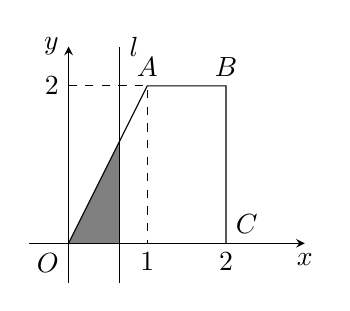
\begin{tikzpicture}[samples=200,>=stealth]
	\fill [gray] (0,0)--(0.65,0)--(0.65,1.3)--cycle;
	\draw [->] (-0.5,0)--(0,0) node [below left] {$O$} --(3,0) node [below] {$x$};
	\draw [->] (0,-0.5)--(0,2.5) node [left] {$y$};
	\draw (0,0)--(1,2) node [above] {$A$}--(2,2) node [above] {$B$}--(2,0) node [above right] {$C$};
	\draw (0.65,-0.5)--(0.65,2.5) node [right] {$l$};
	\draw [dashed] (0,2) node [left] {$2$} --(1,2)--(1,0) node [below] {$1$};
	\draw (2,0) node [below] {$2$};
	
	\end{tikzpicture}
\end{center}
则函数$S=f(t)$的图像大致为\blank{30}.
\fourch{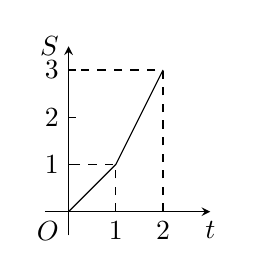
\begin{tikzpicture}[>=stealth]
	\draw [->] (-0.3,0)--(0,0) node [below left] {$O$} --(1.8,0) node [below] {$t$};
	\draw [->] (0,-0.3)--(0,2.1) node [left] {$S$};
	\draw (0.6,0) node [below] {$1$}--(0.6,0.1);
	\draw (1.2,0) node [below] {$2$}--(1.2,0.1);
	\draw (0,0.6) node [left] {$1$}--(0.1,0.6);
	\draw (0,1.2) node [left] {$2$}--(0.1,1.2);
	\draw (0,1.8) node [left] {$3$}--(0.1,1.8);
	\draw (0,0)--(0.6,0.6)--(1.2,1.8);
	\draw [dashed] (0.6,0)--(0.6,0.6)--(0,0.6);
	\draw [dashed] (1.2,0)--(1.2,1.8)--(0,1.8);
	\end{tikzpicture}}{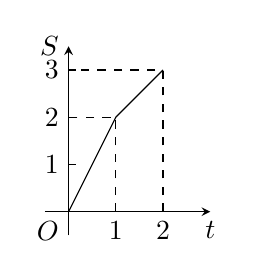
\begin{tikzpicture}[>=stealth]
	\draw [->] (-0.3,0)--(0,0) node [below left] {$O$} --(1.8,0) node [below] {$t$};
	\draw [->] (0,-0.3)--(0,2.1) node [left] {$S$};
	\draw (0.6,0) node [below] {$1$}--(0.6,0.1);
	\draw (1.2,0) node [below] {$2$}--(1.2,0.1);
	\draw (0,0.6) node [left] {$1$}--(0.1,0.6);
	\draw (0,1.2) node [left] {$2$}--(0.1,1.2);
	\draw (0,1.8) node [left] {$3$}--(0.1,1.8);
	\draw (0,0)--(0.6,1.2)--(1.2,1.8);
	\draw [dashed] (0.6,0)--(0.6,1.2)--(0,1.2);
	\draw [dashed] (1.2,0)--(1.2,1.8)--(0,1.8);
	\end{tikzpicture}}{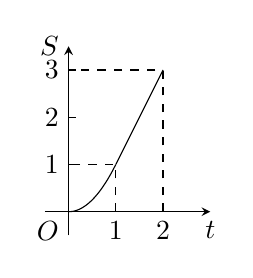
\begin{tikzpicture}[>=stealth,samples=200]
	\draw [->] (-0.3,0)--(0,0) node [below left] {$O$} --(1.8,0) node [below] {$t$};
	\draw [->] (0,-0.3)--(0,2.1) node [left] {$S$};
	\draw (0.6,0) node [below] {$1$}--(0.6,0.1);
	\draw (1.2,0) node [below] {$2$}--(1.2,0.1);
	\draw (0,0.6) node [left] {$1$}--(0.1,0.6);
	\draw (0,1.2) node [left] {$2$}--(0.1,1.2);
	\draw (0,1.8) node [left] {$3$}--(0.1,1.8);
	\draw [domain=0:1] plot ({\x*0.6},{\x*\x*0.6});
	\draw (0.6,0.6)--(1.2,1.8);
	\draw [dashed] (0.6,0)--(0.6,0.6)--(0,0.6);
	\draw [dashed] (1.2,0)--(1.2,1.8)--(0,1.8);
	\end{tikzpicture}}{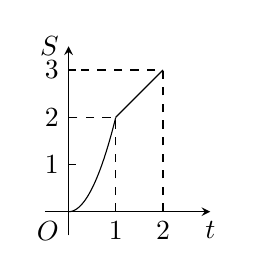
\begin{tikzpicture}[>=stealth,samples=200]
	\draw [->] (-0.3,0)--(0,0) node [below left] {$O$} --(1.8,0) node [below] {$t$};
	\draw [->] (0,-0.3)--(0,2.1) node [left] {$S$};
	\draw (0.6,0) node [below] {$1$}--(0.6,0.1);
	\draw (1.2,0) node [below] {$2$}--(1.2,0.1);
	\draw (0,0.6) node [left] {$1$}--(0.1,0.6);
	\draw (0,1.2) node [left] {$2$}--(0.1,1.2);
	\draw (0,1.8) node [left] {$3$}--(0.1,1.8);
	\draw [domain=0:1] plot ({\x*0.6},{2*\x*\x*0.6});
	\draw (0.6,1.2)--(1.2,1.8);
	\draw [dashed] (0.6,0)--(0.6,1.2)--(0,1.2);
	\draw [dashed] (1.2,0)--(1.2,1.8)--(0,1.8);
	\end{tikzpicture}}


关联目标:

暂未关联目标



标签: 第二单元

答案: 暂无答案

解答或提示: 暂无解答与提示

使用记录:

暂无使用记录


出处: 2016年双基百分百
\item { (003869)}函数$f(x)=a^x+b \ (a>1, \ b<-1)$, 则$y=f^{-1}(x)$的图像一定不经过第\blank{50}象限.


关联目标:

暂未关联目标



标签: 第二单元

答案: 暂无答案

解答或提示: 暂无解答与提示

使用记录:

暂无使用记录


出处: 2016年双基百分百
\item { (003884)}已知函数$y=f(x)$的定义域为$\{x|-3\le x\le 8, \ x\ne 5\}$, 值域为$\{y|-1\le y\le 2, \ y\ne 0\}$. 下列关于函数$y=f(x)$的说法: \textcircled{1} 当$x=-3$时, $y=-1$; \textcircled{2} 将$y=f(x)$的图像补上$(5,0)$, 得到的图像必定是一条连续的曲线; \textcircled{3} $y=f(x)$是$[-3,5)$上的单调函数; \textcircled{4} $y=f(x)$的图像与坐标轴只有一个交点. 其中正确的命题是\blank{50}.


关联目标:

暂未关联目标



标签: 第二单元

答案: 暂无答案

解答或提示: 暂无解答与提示

使用记录:

暂无使用记录


出处: 2016年双基百分百
\item { (003889)}已知函数$f(x)=\begin{cases}ax^2-2x-1, & x\ge 0,\\ x^2+bx+c, & x<0\end{cases}$是偶函数, 直线$y=t$与函数$y=f(x)$的图像自左向右依次交于四个不同点$A,B,C,D$. 若$AB=BC$, 则实数$t$的值为\blank{50}.


关联目标:

暂未关联目标



标签: 第二单元

答案: 暂无答案

解答或提示: 暂无解答与提示

使用记录:

暂无使用记录


出处: 2016年双基百分百
\item { (003894)}对于函数$f(x)=ax^2+(b+1)x+b-2 \ (a\ne 0)$, 若存在实数$x_0$, 使$f(x_0)=x_0$成立, 则称$x_0$为$f(x)$的不动点.\\
(1) 若对于任何实数$b$, 函数$f(x)$恒有两个相异的不动点, 求实数$a$的取值范围;\\
(2) 在(1)的条件下, 若函数$y=f(x)$的图像上$A,B$两点的横坐标是函数$f(x)$的不动点, 且直线$y=kx+\dfrac{1}{2a^2+1}$是线段$AB$的垂直平分线, 求实数$b$的取值范围.


关联目标:

暂未关联目标



标签: 第二单元

答案: 暂无答案

解答或提示: 暂无解答与提示

使用记录:

暂无使用记录


出处: 2016年双基百分百
\item { (003936)}函数$y=\ln(\cos x) \ \left(-\dfrac{\pi}{2}<x<\dfrac{\pi}{2}\right)$的大致图像是\blank{30}.
\fourch{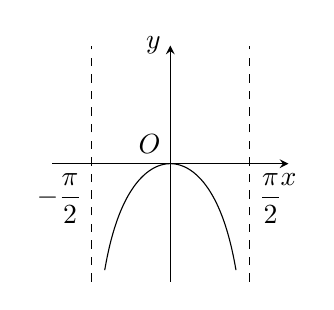
\begin{tikzpicture}[samples=200,>=stealth]
	\draw [->](-1.5,0)--(0,0) node [above left] {$O$}--(1.5,0) node [below] {$x$};
	\draw [->](0,-1.5)--(0,1.5) node [left] {$y$};
	\draw [dashed] (-1,-1.5)--(-1,1.5) (1,-1.5)--(1,1.5);
	\draw (-1,0) node [below left] {$-\dfrac{\pi}{2}$};
	\draw (1,0) node  [below right] {$\dfrac{\pi}{2}$};
	\draw [domain=-75:75] plot ({\x/90},{ln(cos(\x))});
	\end{tikzpicture}}{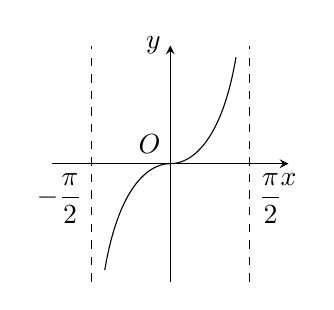
\begin{tikzpicture}[samples=200,>=stealth]
	\draw [->](-1.5,0)--(0,0) node [above left] {$O$}--(1.5,0) node [below] {$x$};
	\draw [->](0,-1.5)--(0,1.5) node [left] {$y$};
	\draw [dashed] (-1,-1.5)--(-1,1.5) (1,-1.5)--(1,1.5);
	\draw (-1,0) node [below left] {$-\dfrac{\pi}{2}$};
	\draw (1,0) node  [below right] {$\dfrac{\pi}{2}$};
	\draw [domain=-75:0] plot ({\x/90},{ln(cos(\x))});
	\draw [domain=0:75] plot ({\x/90},{-ln(cos(\x))});
	\end{tikzpicture}}{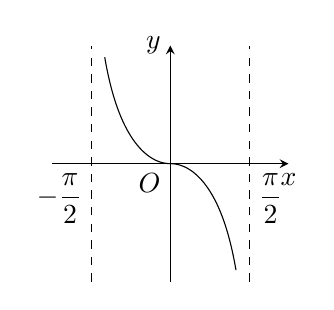
\begin{tikzpicture}[samples=200,>=stealth]
	\draw [->](-1.5,0)--(0,0) node [below left] {$O$}--(1.5,0) node [below] {$x$};
	\draw [->](0,-1.5)--(0,1.5) node [left] {$y$};
	\draw [dashed] (-1,-1.5)--(-1,1.5) (1,-1.5)--(1,1.5);
	\draw (-1,0) node [below left] {$-\dfrac{\pi}{2}$};
	\draw (1,0) node  [below right] {$\dfrac{\pi}{2}$};
	\draw [domain=-75:0] plot ({\x/90},{-ln(cos(\x))});
	\draw [domain=0:75] plot ({\x/90},{ln(cos(\x))});
	\end{tikzpicture}}{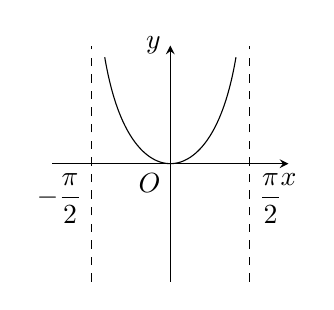
\begin{tikzpicture}[samples=200,>=stealth]
	\draw [->](-1.5,0)--(0,0) node [below left] {$O$}--(1.5,0) node [below] {$x$};
	\draw [->](0,-1.5)--(0,1.5) node [left] {$y$};
	\draw [dashed] (-1,-1.5)--(-1,1.5) (1,-1.5)--(1,1.5);
	\draw (-1,0) node [below left] {$-\dfrac{\pi}{2}$};
	\draw (1,0) node  [below right] {$\dfrac{\pi}{2}$};
	\draw [domain=-75:75] plot ({\x/90},{-ln(cos(\x))});
	\end{tikzpicture}}


关联目标:

暂未关联目标



标签: 第二单元

答案: 暂无答案

解答或提示: 暂无解答与提示

使用记录:

暂无使用记录


出处: 2016年双基百分百
\item { (004000)}请根据图中的函数图像, 将下列数值按从小到大的顺序排列:\blank{50}.
\begin{center}
    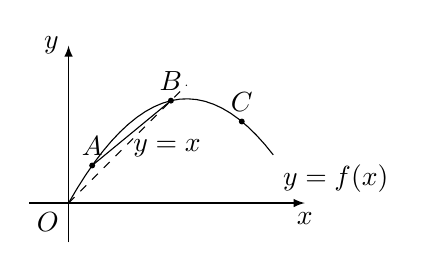
\begin{tikzpicture}[>=latex]
        \draw [->] (-0.5,0) -- (3,0) node [below] {$x$};
        \draw [->] (0,-0.5) -- (0,2) node [left] {$y$};
        \draw (0,0) node [below left] {$O$};
        \draw [domain = 0:2.6, name path = curve] plot (\x,{\x*(3-\x)/1.7}) node [below right] {$y=f(x)$};
        \draw [dashed] (0,0) -- (1.5,1.5);
        \filldraw (1.3,1.3) circle (0.03) node [above] {$B$} -- (0.3,{0.3*2.7/1.7}) circle (0.03) node [above] {$A$};
        \filldraw (2.2,{2.2*0.8/1.7}) circle (0.03) node [above] {$C$};
        \draw (0.7,0.7) node [right] {$y=x$};
    \end{tikzpicture}    
\end{center}
\textcircled{1} 曲线在点$A$处切线的斜率;\\
\textcircled{2} 曲线在点$B$处切线的斜率;\\
\textcircled{3} 曲线在点$C$处切线的斜率;\\
\textcircled{4} 割线$AB$的斜率;\\
\textcircled{5} 数值$0$;\\
\textcircled{6} 数值$1$.


关联目标:

K0701001X|D07001X|经历在平面直角坐标系中探索确定直线位置的几何要素, 理解直线的倾斜角和斜率的概念.

K0228001X|D02005X|了解一般曲线的切线可定义为割线的极限情形.



标签: 第二单元

答案: 暂无答案

解答或提示: 暂无解答与提示

使用记录:

暂无使用记录


出处: 教材复习题
\item { (004007)}已知$y=f'(x)$的图像如图所示, 求函数$y=f(x)$在$(-2,2)$上的单调区间和极值点.
\begin{center}
    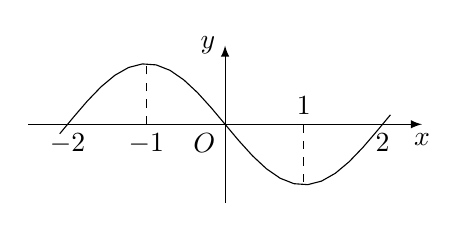
\begin{tikzpicture}[>=latex]
        \draw [->] (-2.5,0) -- (2.5,0) node [below] {$x$};
        \draw [->] (0,-1) -- (0,1) node [left] {$y$};
        \draw (0,0) node [below left] {$O$};
        \draw [domain = -2.1:2.1] plot (\x, {-sin(\x*90)/1.3});
        \draw [dashed] (-1,0) node [below] {$-1$} -- (-1,{1/1.3}) (1,0) node [above] {$1$}-- (1,{-1/1.3});
        \draw (-2,0) node [below] {$-2$} (2,0) node [below] {$2$};
    \end{tikzpicture}
\end{center}


关联目标:

K0220001B|D02003B|理解单调函数、单调区间的定义.

K0233001X|D02006X|结合图像直观, 理解极大值与极大值点, 极小值与极小值点、极值与极值点的定义.



标签: 第二单元

答案: 暂无答案

解答或提示: 暂无解答与提示

使用记录:

暂无使用记录


出处: 教材复习题
\item { (004009)}设函数$y=x^3+ax^2+bx+c$的图像与$y=0$在原点相切, 若函数的极小值为$-4$, 求函数的表达式与单调减区间.


关联目标:

K0228003X|D02005X|用代数语言描述函数图像上某点处割线斜率的极限, 进而结合导数的定义, 理解切线的斜率就是函数在该点处的导数.

K0233003X|D02006X|会通过求导求得不超过三次的多项式函数与简单三角函数的极值点与极值.



标签: 第二单元

答案: 暂无答案

解答或提示: 暂无解答与提示

使用记录:

暂无使用记录


出处: 教材复习题
\item { (004067)}已知定义在$\mathbf{R}$上的函数$f(x)$满足: \textcircled{1} $f(x)+f(2-x)=0$; \textcircled{2} $f(x)-f(-2-x)=0$; \textcircled{3} 在$[-1,1]$上表达式为$f(x)=\begin{cases} \sqrt{1-x^2}, & x\in [-1,0], \\ 1-x, & x\in (0,1], \end{cases}$ 则函数$f(x)$与$g(x)=\begin{cases} {2^x}, & x\le 0 \\ \log_\frac 12x, & x>0 \end{cases}$的图像在区间$[-3,3]$上的交点的个数为\blank{50}.


关联目标:

暂未关联目标



标签: 第二单元

答案: $6$

解答或提示: 暂无解答与提示

使用记录:

20220301	2022届高三1班	\fcolorbox[rgb]{0,0,0}{1.000,0.838,0}{0.581}


出处: 2022届高三下学期测验卷01第9题
\item { (004070)}已知$f(x)=2x^2+2x+b$是定义在$[-1,0]$上的函数, 若$f[f(x)]\le 0$在定义域上恒成立, 而且存在实数$x_0$满足: $f[f(x_0)]=x_0$且$f(x_0)\ne x_0$, 则实数$b$的取值范围是\blank{50}.


关联目标:

暂未关联目标



标签: 第二单元

答案: $[-\dfrac12,-\dfrac 38)$

解答或提示: 暂无解答与提示

使用记录:

20220301	2022届高三1班	\fcolorbox[rgb]{0,0,0}{0.000,1.000,0}{0.000}


出处: 2022届高三下学期测验卷01第12题
\item { (004089)}$[x]$是不超过$x$的最大整数, 则方程$(2^x)^2-\dfrac 74\cdot [2^x]-\dfrac 14=0$满足$x<1$的所有实数解是\blank{50}.


关联目标:

暂未关联目标



标签: 第二单元

答案: 暂无答案

解答或提示: 暂无解答与提示

使用记录:

20220308	2022届高三1班	\fcolorbox[rgb]{0,0,0}{1.000,0.186,0}{0.907}


出处: 2022届高三下学期测验卷02第10题
\item { (004097)}已知函数$f(x)=1-\dfrac 6{a^{x+1}+a}$($a>0$, $a\ne 1$)是定义在$\mathbf{R}$上的奇函数.\\
(1) 求实数$a$的值及函数$f(x)$的值域;\\
(2) 若不等式 $t\cdot f(x)\ge 3^x-3$在$x\in [1,2]$上恒成立, 求实数$t$的取值范围.


关联目标:

暂未关联目标



标签: 第二单元

答案: 暂无答案

解答或提示: 暂无解答与提示

使用记录:

20220308	2022届高三1班	\fcolorbox[rgb]{0,0,0}{1.000,0.032,0}{0.984}	\fcolorbox[rgb]{0,0,0}{1.000,0.104,0}{0.948}


出处: 2022届高三下学期测验卷02第18题
\item { (004151)}设不等式组$\begin{cases} x+y-6\ge 0, \\ x-y+2\ge 0, \\ x-3y+6\le 0 \end{cases}$表示的可行域为$\Omega$, 若指数函数$y=a^x$的图像与$\Omega$有公共点, 则$a$的取值范围是\blank{50}.


关联目标:

暂未关联目标



标签: 第二单元

答案: 暂无答案

解答或提示: 暂无解答与提示

使用记录:

20220407	2022届高三1班	\fcolorbox[rgb]{0,0,0}{1.000,0.418,0}{0.791}


出处: 2022届高三下学期测验卷05第9题
\item { (004184)}设$m$为给定的实常数, 若函数$y=f(x)$在其定义域内存在实数$x_0$, 使得$f(x_0+m)=f(x_0)+f(m)$成立, 则称函数$f(x)$为``$G(m)$函数''.\\
(1) 若函数$f(x)=2^x$为``$G(2)$函数'', 求实数$x_0$的值;\\
(2) 若函数$f(x)=\lg \dfrac a{x^2+1}$为``$G(1)$函数'', 求实数$a$的取值范围;\\
(3) 已知$f(x)=x+b$($b\in \mathbf{R}$)为``$G(0)$函数'', 设$g(x)=x|x-4|$. 若对任意的$x_1,x_2\in[0,t]$, 当$x_1\ne x_2$时, 都有$\dfrac{g(x_1)-g(x_2)}{f(x_1)-f(x_2)}>2$成立, 求实数$t$的最大值.


关联目标:

暂未关联目标



标签: 第二单元

答案: 暂无答案

解答或提示: 暂无解答与提示

使用记录:

20220421	2022届高三1班	\fcolorbox[rgb]{0,0,0}{1.000,0.012,0}{0.994}	\fcolorbox[rgb]{0,0,0}{1.000,0.520,0}{0.740}	\fcolorbox[rgb]{0,0,0}{1.000,0.734,0}{0.633}


出处: 2022届高三下学期测验卷06第21题
\item { (004214)}设定义域为$\mathbf{R}$的函数$f(x)$、$g(x)$都有反函数, 且函数$f(x-1)$和$g^{-1}(x-3)$图像关于直线$y=x$对称, 若$g(5)=2015$, 则$f(4)=$\blank{50}.


关联目标:

暂未关联目标



标签: 第二单元

答案: 暂无答案

解答或提示: 暂无解答与提示

使用记录:

20220505	2022届高三1班	\fcolorbox[rgb]{0,0,0}{1.000,0.046,0}{0.977}


出处: 2022届高三下学期测验卷08第9题
\item { (004220)}已知函数\textcircled{1} $f(x)=3\ln x$; \textcircled{2} $f(x)=3\mathrm{e}^{\cos x}$; \textcircled{3} $f(x)=3\mathrm{e}^x$; \textcircled{4} $f(x)=3\cos x$; 其中对于$f(x)$定义域内的任意一个自变量$x_1$都存在唯一一个自变量$x_2$, 使$\sqrt{f(x_1)f(x_2)}=3$成立的函数是\bracket{20}.
\fourch{\textcircled{3}}{\textcircled{2}\textcircled{3}}{\textcircled{1}\textcircled{2}\textcircled{4}}{\textcircled{4}}


关联目标:

暂未关联目标



标签: 第二单元|第三单元

答案: 暂无答案

解答或提示: 暂无解答与提示

使用记录:

20220505	2022届高三1班	\fcolorbox[rgb]{0,0,0}{1.000,0.140,0}{0.930}


出处: 2022届高三下学期测验卷08第15题
\item { (004224)}对于两个定义域相同的函数$f(x)$、$g(x)$, 若存在实数$m$、$n$, 使$h(x)=mf(x)+ng(x)$, 则称函数$h(x)$是由``基函数$f(x)$、$g(x)$''生成的.\\
(1) $f(x)=x^2+3x$和$g(x)=3x+4$生成一个偶函数$h(x)$, 求$h(2)$的值;\\
(2) 若$h(x)=2x^2+3x-1$由$f(x)=x^2+ax$, $g(x)=x+b$($a,b\in \mathbf{R}$且$ab\ne 0$)生成, 求$a+2b$的取值范围.


关联目标:

暂未关联目标



标签: 第二单元

答案: 暂无答案

解答或提示: 暂无解答与提示

使用记录:

20220505	2022届高三1班	\fcolorbox[rgb]{0,0,0}{1.000,0.100,0}{0.950}	\fcolorbox[rgb]{0,0,0}{1.000,0.486,0}{0.757}


出处: 2022届高三下学期测验卷08第19题
\item { (004228)}函数$f(x)=\sqrt{1-\dfrac 2x}$的定义域是\blank{50}.


关联目标:

暂未关联目标



标签: 第二单元

答案: 暂无答案

解答或提示: 暂无解答与提示

使用记录:

20220512	2022届高三1班	\fcolorbox[rgb]{0,0,0}{1.000,0.232,0}{0.884}


出处: 2022届高三下学期测验卷09第2题
\item { (004270)}函数$f(x)=\sqrt{\dfrac{1-x}{3+x}}$的定义域为\blank{50}.


关联目标:

暂未关联目标



标签: 第二单元

答案: 暂无答案

解答或提示: 暂无解答与提示

使用记录:

20220524	2022届高三1班	\fcolorbox[rgb]{0,0,0}{1.000,0.094,0}{0.953}


出处: 2022届高三下学期测验卷11第2题
\item { (004272)}已知函数$g(x)$的图像与函数$f(x)=\log_2(3^x-1)$的图像关于直线$y=x$对称,则$g(3)=$\blank{50}.


关联目标:

暂未关联目标



标签: 第二单元

答案: 暂无答案

解答或提示: 暂无解答与提示

使用记录:

20220524	2022届高三1班	\fcolorbox[rgb]{0,0,0}{1.000,0.046,0}{0.977}


出处: 2022届高三下学期测验卷11第4题
\item { (004289)}已知函数$f(x)$的定义域为$D$, 若存在实常数$\lambda$及$a$($a\ne 0$), 对任意$x\in D$, 当$x+a\in D$且$x-a\in D$时, 都有$f(x+a)+f(x-a)=\lambda f(x)$成立, 则称函数$f(x)$具有性质$M(\lambda,a)$.\\
(1) 判断函数$f(x)=x^2$是否具有性质$M(\lambda,a)$, 并说明理由;\\
(2) 若函数$g(x)=\sin 2x+\sin x$具有性质$M(\lambda,a)$, 求$\lambda$及$a$应满足的条件;\\
(3) 已知定义域为$\mathbf{R}$的函数$y=h(x)$不存在零点, 且具有性质$M(t+\dfrac{1}{t},t)$(其中$t>0$, $t\ne 1$), 记$a_n=h(n)$($n\in \mathbf{N}^*$), 求证: 数列$\{a_n\}$为等比数列的充要条件是$\dfrac{a_2}{a_1}=t$或$\dfrac{a_2}{a_1}=\dfrac{1}{t}$.


关联目标:

暂未关联目标



标签: 第二单元

答案: 暂无答案

解答或提示: 暂无解答与提示

使用记录:

20220524	2022届高三1班	\fcolorbox[rgb]{0,0,0}{1.000,0.186,0}{0.907}	\fcolorbox[rgb]{0,0,0}{1.000,0.984,0}{0.508}	\fcolorbox[rgb]{0,0,0}{0.890,1.000,0}{0.445}


出处: 2022届高三下学期测验卷11第21题
\item { (004305)}定义$F(a,b)=\begin{cases} a, & a \le b, \\ b, & a>b,\end{cases}$, 已知函数$f(x)$、$g(x)$定义域都是$\mathbf{R}$, 给出下列命题:\\
(1) 若$f(x)$、$g(x)$都是奇函数, 则函数$F(f(x),g(x))$为奇函数;\\
(2) 若$f(x)$、$g(x)$都是减函数, 则函数$F(f(x),g(x))$为减函数;\\
(3) 若$f_{\min}(x)=m$, $g_{\min}(x)=n$, 则$F_{\min}(f(x),g(x))=F(m,n)$;\\
(4) 若$f(x)$、$g(x)$都是周期函数, 则函数$F(f(x),g(x))$是周期函数.\\
其中正确命题的个数为\bracket{20}.
\fourch{$1$个}{$2$个}{$3$个}{$4$个}


关联目标:

暂未关联目标



标签: 第二单元

答案: 暂无答案

解答或提示: 暂无解答与提示

使用记录:

20220607	2022届高三1班	\fcolorbox[rgb]{0,0,0}{0.512,1.000,0}{0.256}


出处: 2022届高三下学期测验卷12第16题
\item { (004313)}设$a\in \mathbf{R}$. 若$a$使得函数$f(x)=\sqrt{8-ax-2x^2}$是偶函数, 则函数$y=f(x)$的定义域是\blank{50}.


关联目标:

暂未关联目标



标签: 第二单元

答案: 暂无答案

解答或提示: 暂无解答与提示

使用记录:

20220627	2022届高三1班	\fcolorbox[rgb]{0,0,0}{1.000,0.000,0}{1.000}


出处: 2022届高三下学期测验卷13第3题
\item { (004332)}函数$y=\log_2(x-2)$的定义域为\blank{50}.


关联目标:

暂未关联目标



标签: 第二单元

答案: 暂无答案

解答或提示: 暂无解答与提示

使用记录:

20220630	2022届高三1班	\fcolorbox[rgb]{0,0,0}{1.000,0.000,0}{1.000}


出处: 2022届高三下学期测验卷14第1题
\item { (004335)}幂函数$y=x^k$的图像经过点$(4,\dfrac 12)$, 则它的单调减区间为\blank{50}.


关联目标:

暂未关联目标



标签: 第二单元

答案: 暂无答案

解答或提示: 暂无解答与提示

使用记录:

20220630	2022届高三1班	\fcolorbox[rgb]{0,0,0}{1.000,0.000,0}{1.000}


出处: 2022届高三下学期测验卷14第4题
\item { (004339)}已知偶函数$y=f(x)$的定义域为$\mathbf{R}$, 且当$x\ge 0$时, $f(x)=x-4$, 则不等式$xf(x)\le 5$的解为\blank{50}.


关联目标:

暂未关联目标



标签: 第二单元

答案: 暂无答案

解答或提示: 暂无解答与提示

使用记录:

20220630	2022届高三1班	\fcolorbox[rgb]{0,0,0}{1.000,0.326,0}{0.837}


出处: 2022届高三下学期测验卷14第8题
\item { (004347)}已知$y=f(x)$与$y=g(x)$皆是定义域、值域均为$\mathbf{R}$的函数. 若对任意$x\in \mathbf{R}$, $f(x)>g(x)$恒成立, 且$y=f(x)$与$y=g(x)$的反函数$y=f^{-1}(x)$、$y=g^{-1}(x)$均存在. 命题$P$: ``对任意$x\in \mathbf{R}$, $f^{-1}(x)<g^{-1}(x)$恒成立''; 命题$Q$: ``函数$y=f(x)+g(x)$的反函数一定存在''. 以下关于这两个命题的真假判断, 正确的是\bracket{20}.
\twoch{命题$P$真, 命题$Q$真}{命题$P$真, 命题$Q$假
}{命题$P$假, 命题$Q$真}{命题$P$假, 命题$Q$假}


关联目标:

暂未关联目标



标签: 第二单元

答案: 暂无答案

解答或提示: 暂无解答与提示

使用记录:

20220630	2022届高三1班	\fcolorbox[rgb]{0,0,0}{0.884,1.000,0}{0.442}


出处: 2022届高三下学期测验卷14第16题
\item { (004368)}已知函数$y=f(x)$的定义域为$(0,+\infty)$, 满足对任意$x\in (0,+\infty)$, 恒有$f[f(x)-\dfrac 1x]=4$. 若函数$y=f(x)-4$的零点个数为有限的$n$($n\in \mathbf{N}^*$)个, 则$n$的最大值为\bracket{20}.
\fourch{$1$}{$2$}{$3$}{$4$}


关联目标:

暂未关联目标



标签: 第二单元

答案: 暂无答案

解答或提示: 暂无解答与提示

使用记录:

20210918	2022届高三1班	\fcolorbox[rgb]{0,0,0}{1.000,0.744,0}{0.628}


出处: 2022届高三上学期测验卷01第16题
\item { (004377)}函数$f(x)=\sqrt{\dfrac{1-x}x}$的定义域为\blank{50}.


关联目标:

暂未关联目标



标签: 第二单元

答案: 暂无答案

解答或提示: 暂无解答与提示

使用记录:

20210928	2022届高三1班	\fcolorbox[rgb]{0,0,0}{1.000,0.000,0}{1.000}


出处: 2022届高三上学期测验卷02第4题
\item { (004380)}已知函数$f(x)$的定义域为$\mathbf{R}$, 满足对任意$x\in \mathbf{R}$, 恒有$f(x)+f(x+2)=4$. 若$f(1)+f(2)=1$, 则$f(2021)-f(2020)=$\blank{50}.


关联目标:

暂未关联目标



标签: 第二单元

答案: 暂无答案

解答或提示: 暂无解答与提示

使用记录:

20210928	2022届高三1班	\fcolorbox[rgb]{0,0,0}{1.000,0.046,0}{0.977}


出处: 2022届高三上学期测验卷02第7题
\item { (004385)}设函数$f(x)$的定义域为$\mathbf{R}$, $f(x)$满足对任意$x_1,x_2\in \mathbf{R}$, 当$x_1\ne x_2$时, 恒有$|f(x_1)-f(x_2)|>2|x_1-x_2|$. 对于命题: \textcircled{1} $f(x)$的解析式可以是$f(x)=x^3+2021x$; \textcircled{2} $f(x)$的解析式可以是$f(x)=2021^{-x}$, 下列判断正确的是\bracket{20}.
\twoch{\textcircled{1}、\textcircled{2}均为真命题}{\textcircled{1}、\textcircled{2}均为假命题}{\textcircled{1}为真命题、\textcircled{2}为假命题}{\textcircled{1}为假命题、\textcircled{2}为真命题}


关联目标:

暂未关联目标



标签: 第二单元

答案: 暂无答案

解答或提示: 暂无解答与提示

使用记录:

20210928	2022届高三1班	\fcolorbox[rgb]{0,0,0}{1.000,0.000,0}{1.000}


出处: 2022届高三上学期测验卷02第12题
\item { (004387)}设函数$f(x)$的定义域为$(0,+\infty)$, 若对任意$x\in (0,+\infty)$, 恒有$f(2x)=2f(x)$, 则称$f(x)$为``$2$阶缩放函数''.\\
(1) 已知函数$f(x)$为``$2$阶缩放函数'', 当$x\in (1,2]$时, $f(x)=1-\log_2 x$, 求$f(2\sqrt{2})$的值;\\
(2) 已知函数$f(x)$为``$2$阶缩放函数'', 当$x\in (1,2]$时, $f(x)=\sqrt{2x-x^2}$, 求证: 函数$y=f(x)-x$在$(1,+\infty)$上无零点.


关联目标:

暂未关联目标



标签: 第二单元

答案: 暂无答案

解答或提示: 暂无解答与提示

使用记录:

20210928	2022届高三1班	\fcolorbox[rgb]{0,0,0}{1.000,0.018,0}{0.991}	\fcolorbox[rgb]{0,0,0}{1.000,0.298,0}{0.851}


出处: 2022届高三上学期测验卷02第14题
\item { (004389)}函数$f(x)=x^{- \frac 12}$的定义域为\blank{50}.


关联目标:

暂未关联目标



标签: 第二单元

答案: 暂无答案

解答或提示: 暂无解答与提示

使用记录:

20211012	2022届高三1班	\fcolorbox[rgb]{0,0,0}{1.000,0.046,0}{0.977}


出处: 2022届高三上学期测验卷03第2题
\item { (004401)}下列函数中, 值域为$(0,+\infty)$的是\bracket{20}.
\fourch{$y=x^2$}{$y=\dfrac 2x$}{$y=2^x$}{$y=|\log_2x|$}


关联目标:

暂未关联目标



标签: 第二单元

答案: 暂无答案

解答或提示: 暂无解答与提示

使用记录:

20211012	2022届高三1班	\fcolorbox[rgb]{0,0,0}{1.000,0.090,0}{0.955}


出处: 2022届高三上学期测验卷03第14题
\item { (004403)}设集合$A=\{y|y=a^x,\ x>0\}$(其中常数$a>0,  \ a\ne 1$), $B=\{y|y=x^k,\ x\in A\}$(其中常数$k\in \mathbf{Q}$), 则``$k<0$''是``$A\cap B=\varnothing$''的\bracket{20}.
\twoch{充分非必要条件}{必要非充分条件}{充分必要条件}{既非充分又非必要条件}


关联目标:

K0106003B|D01002B|能基于推出关系有理有据地判定熟悉的陈述句之间的必要条件关系、充分条件关系和充要条件关系.

K0215001B|D02003B|理解函数的概念, 体会函数即数与数之间的对应关系, 理解函数的定义(包含自变量、函数值、定义域、值域的概念).



标签: 第一单元|第二单元

答案: 暂无答案

解答或提示: 暂无解答与提示

使用记录:

20211012	2022届高三1班	\fcolorbox[rgb]{0,0,0}{1.000,0.954,0}{0.523}


出处: 2022届高三上学期测验卷03第16题
\item { (004408)}记函数$f(x)$的定义域为$D$. 如果存在实数$a$、$b$使得$f(a-x)+f(a+x)=b$对任意满足$a-x\in D$且$a+x\in D$的$x$恒成立, 则称$f(x)$为$\Psi$函数.\\
(1) 设函数$f(x)=\dfrac 1x-1$, 试判断$f(x)$是否为$\Psi$函数, 若是求出$a,b$, 若不是请说明理由;\\
(2) 设函数$g(x)=\dfrac 1{2^x+t}$, 其中常数$t\ne 0$, 证明: $g(x)$是$\Psi$函数;\\
(3) 若$h(x)$是定义在$\mathbf{R}$上的$\Psi$函数, 且函数$h(x)$的图像关于直线$x=m$($m$为常数)对称, 试判断$h(x)$是否为周期函数? 并证明你的结论.


关联目标:

暂未关联目标



标签: 第二单元

答案: 暂无答案

解答或提示: 暂无解答与提示

使用记录:

20211012	2022届高三1班	\fcolorbox[rgb]{0,0,0}{1.000,0.750,0}{0.625}	\fcolorbox[rgb]{0,0,0}{0.690,1.000,0}{0.345}	\fcolorbox[rgb]{0,0,0}{0.482,1.000,0}{0.241}


出处: 2022届高三上学期测验卷03第21题
\item { (004411)}若函数$y=\log_2(x-m)+1$的反函数的图像经过点$(1,3)$, 则实数$m=$\blank{50}.


关联目标:

暂未关联目标



标签: 第二单元

答案: 暂无答案

解答或提示: 暂无解答与提示

使用记录:

20211018	2022届高三1班	\fcolorbox[rgb]{0,0,0}{1.000,0.096,0}{0.952}


出处: 2022届高三上学期测验卷04第3题
\item { (004412)}函数$f(x)=x+\dfrac 1{x-2}$的值域是\blank{50}.


关联目标:

暂未关联目标



标签: 第二单元

答案: 暂无答案

解答或提示: 暂无解答与提示

使用记录:

20211018	2022届高三1班	\fcolorbox[rgb]{0,0,0}{1.000,0.238,0}{0.881}


出处: 2022届高三上学期测验卷04第4题
\item { (004417)}函数$f(x)=\dfrac x{x+1}+\dfrac{x+1}{x+2}+\dfrac{x+2}{x+3}$图像的对称中心的坐标是\blank{50}.


关联目标:

暂未关联目标



标签: 第二单元

答案: 暂无答案

解答或提示: 暂无解答与提示

使用记录:

20211018	2022届高三1班	\fcolorbox[rgb]{0,0,0}{1.000,0.380,0}{0.810}


出处: 2022届高三上学期测验卷04第9题
\item { (004424)}设$\mu (x)$表示不小于$x$的最小整数, 例如$\mu(0.3)=1$, $\mu(-2.5)=2$.\\
(1) 解方程$\mu(x-1)=3$;\\
(2) 设$f(x)=\mu (x\cdot \mu (x))$, $n\in \mathbf{N}^*$, 试分别求出$f(x)$在区间$(0,1]$、$(1,2]$以及$(2,3]$上的值域; 若$f(x)$在区间$(0,n]$上的值域为$M_n$, 求集合$M_n$中的元素的个数;\\
(3) 设实数$a>0$, $g(x)=x+a\cdot \dfrac{\mu (x)}x-2$, $h(x)=\dfrac{\sin (\pi x)+2}{x^2-5x+7}$, 若对于任意$x_1,x_2\in (2,4]$都有$g(x_1)>h(x_2)$, 求实数$a$的取值范围.


关联目标:

暂未关联目标



标签: 第二单元

答案: 暂无答案

解答或提示: 暂无解答与提示

使用记录:

20211018	2022届高三1班	\fcolorbox[rgb]{0,0,0}{1.000,0.226,0}{0.887}	\fcolorbox[rgb]{0,0,0}{1.000,0.666,0}{0.667}	\fcolorbox[rgb]{0,0,0}{1.000,0.960,0}{0.520}


出处: 2022届高三上学期测验卷04第16题
\item { (004425)}函数$y=\log_2(4-x^2)$的定义域是\blank{50}.


关联目标:

暂未关联目标



标签: 第二单元

答案: 暂无答案

解答或提示: 暂无解答与提示

使用记录:

20211026	2022届高三1班	\fcolorbox[rgb]{0,0,0}{1.000,0.000,0}{1.000}


出处: 2022届高三上学期测验卷05第1题
\item { (004429)}已知函数$f(x)=a\cdot 2^x+3-a$($a\in \mathbf{R}$且$a\ne 0$)的反函数为$y=f^{-1}(x)$, 则函数$y=f^{-1}(x)$的图像经过的定点的坐标为\blank{50}.


关联目标:

暂未关联目标



标签: 第二单元

答案: 暂无答案

解答或提示: 暂无解答与提示

使用记录:

20211026	2022届高三1班	\fcolorbox[rgb]{0,0,0}{1.000,0.046,0}{0.977}


出处: 2022届高三上学期测验卷05第5题
\item { (004435)}集合$A=\{y|y=\log_{\frac 12}x-x,1\le x\le 2\}$, $B=\{x|x^2-5tx+1\le 0\}$, 若$A\cap B=A$, 则实数$t$的取值范围是\blank{50}.


关联目标:

K0215001B|D02003B|理解函数的概念, 体会函数即数与数之间的对应关系, 理解函数的定义(包含自变量、函数值、定义域、值域的概念).

K0114001B|D01004B|掌握结合一元二次函数的图像求解一元二次不等式的方法.

K0104001B|D01001B|理解两个集合的交集的含义, 在具体数学情境中, 能求两个集合的交集.



标签: 第一单元|第二单元

答案: 暂无答案

解答或提示: 暂无解答与提示

使用记录:

20211026	2022届高三1班	\fcolorbox[rgb]{0,0,0}{1.000,0.326,0}{0.837}


出处: 2022届高三上学期测验卷05第11题
\item { (004436)}若定义在实数集$\mathbf{R}$上的奇函数$y=f(x)$的图像关于直线$x=1$对称, 且当$0\le x\le 1$时, $f(x)=x^{\frac 13}$, 则方程$f(x)=\dfrac 13$在区间$(-4,10)$内的所有实根之和为\blank{50}.


关联目标:

暂未关联目标



标签: 第二单元

答案: 暂无答案

解答或提示: 暂无解答与提示

使用记录:

20211026	2022届高三1班	\fcolorbox[rgb]{0,0,0}{1.000,0.326,0}{0.837}


出处: 2022届高三上学期测验卷05第12题
\item { (004440)}已知函数$f(x)=\begin{cases}\log_{\frac 12}(1-x), & -1\le x\le n,  \\ 2^{2-|x-1|}-3, & n<x\le m,  \end{cases}$($n<m$)的值域是$[-1,1]$, 有下列结论:
\textcircled{1} 当$n=0$时, $m$的取值范围为$(0,2]$; \textcircled{2}  当$n=\dfrac 12$时, $m$的取值范围为$(\dfrac 12,2]$; \textcircled{3}  当$n\in [0,\dfrac 12)$时, $m$的取值范围为$[1,2]$; \textcircled{4}  当$n\in [0,\dfrac 12)$时, $m$的取值范围为$(n,2]$;
其中结论正确的所有的序号是\bracket{20}.
\fourch{\textcircled{1}\textcircled{2}}{\textcircled{3}\textcircled{4}}{\textcircled{2}\textcircled{3}}{\textcircled{2}\textcircled{4}}


关联目标:

暂未关联目标



标签: 第二单元

答案: 暂无答案

解答或提示: 暂无解答与提示

使用记录:

20211026	2022届高三1班	\fcolorbox[rgb]{0,0,0}{1.000,0.838,0}{0.581}


出处: 2022届高三上学期测验卷05第16题
\item { (004444)}定义区间$(m,n)$、$[m,n]$、$(m,n]$、$[m,n)$的长度均为$n-m$, 已知不等式$\dfrac 7{6-x}\ge 1$的解集为$A$.\\
(1) 求$A$的长度;\\
(2) 函数$f(x)=\dfrac{(a^2+a)x-1}{a^2x}$($a\in \mathbf{R}$, $a\ne 0$)的定义域与值域都是$[m,n]$($n>m$), 求区间$[m,n]$的最大长度;\\
(3) 关于$x$的不等式$\log_2x+\log_2(tx+3t)<2$的解集为$B$, 若$A\cap B$的长度为$6$, 求实数$t$的取值范围.


关联目标:

暂未关联目标



标签: 第二单元

答案: 暂无答案

解答或提示: 暂无解答与提示

使用记录:

20211026	2022届高三1班	\fcolorbox[rgb]{0,0,0}{1.000,0.116,0}{0.942}	\fcolorbox[rgb]{0,0,0}{1.000,0.472,0}{0.764}	\fcolorbox[rgb]{0,0,0}{0.954,1.000,0}{0.477}


出处: 2022届高三上学期测验卷05第20题
\item { (004445)}对于函数$y=f(x)$($x\in D$), 如果存在实数$a$、$b$($a\ne 0$, 且$a=1$, $b=0$不同时成立), 使得$f(x)=f(ax+b)$对$x\in D$恒成立, 则称函数$f(x)$为``$(a,b)$映像函数''.\\
(1) 判断函数$f(x)=x^2-2$是否是``$(a,b)$映像函数'', 如果是, 请求出相应的$a$、$b$的值, 若不是, 请说明理由;\\
(2) 已知函数$y=f(x)$是定义在$[0,+\infty)$上的``$(2,1)$映像函数'', 且当$x\in [0,1)$时, $f(x)=2^x$, 求函数$y=f(x)$($x\in [3,7)$)的反函数;\\
(3) 在(2)的条件下, 试构造一个数列$\{a_n\}$, 使得当$x\in [a_n,{a_{n+1}})$($n\in \mathbf{N}^*$)时, $2x+1$的取值范围为$[{a_{n+1}},{a_{n+2}})$, 并求$x\in [a_n,{a_{n+1}})$($n\in \mathbf{N}^*$)时, 函数$y=f(x)$的解析式, 及$y=f(x)$($x\in [0,+\infty)$)的值域.


关联目标:

暂未关联目标



标签: 第二单元

答案: 暂无答案

解答或提示: 暂无解答与提示

使用记录:

20211026	2022届高三1班	\fcolorbox[rgb]{0,0,0}{1.000,0.466,0}{0.767}	\fcolorbox[rgb]{0,0,0}{1.000,0.202,0}{0.899}	\fcolorbox[rgb]{0,0,0}{1.000,0.820,0}{0.590}


出处: 2022届高三上学期测验卷05第21题
\item { (004446)}函数$y=\sqrt{2+x}$的定义域为\blank{50}.


关联目标:

暂未关联目标



标签: 第二单元

答案: 暂无答案

解答或提示: 暂无解答与提示

使用记录:

20211102	2022届高三1班	\fcolorbox[rgb]{0,0,0}{1.000,0.048,0}{0.976}


出处: 2022届高三上学期测验卷06第1题
\item { (004452)}已知幂函数$y=f(x)$的图像经过点$P(4,2)$, 则它的反函数为$f^{-1}(x)=$\blank{50}.


关联目标:

暂未关联目标



标签: 第二单元

答案: 暂无答案

解答或提示: 暂无解答与提示

使用记录:

20211102	2022届高三1班	\fcolorbox[rgb]{0,0,0}{1.000,0.524,0}{0.738}


出处: 2022届高三上学期测验卷06第7题
\item { (004496)}已知函数$y=f(x)$存在反函数$y=f^{-1}(x)$, 若函数$y=f(x)+2^x$的图像经过点$(1,4)$, 则函数$y=f^{-1}(x)+\log_2x$的图像必过点\blank{50}.


关联目标:

暂未关联目标



标签: 第二单元

答案: 暂无答案

解答或提示: 暂无解答与提示

使用记录:

20211123	2022届高三1班	\fcolorbox[rgb]{0,0,0}{1.000,0.000,0}{1.000}


出处: 2022届高三上学期测验卷08第8题
\item { (004500)}对于定义域为$D$的函数$f(x)$, 若存在$x_1,x_2\in D$且$x_1\ne x_2$, 使得$f(x_1^2)=f(x_2^2)=2f(x_1+x_2)$, 则称函数$f(x)$具有性质$M$. 若函数$g(x)=|\log_2x-1|$, $x\in (0,a]$具有性质$M$, 则实数$a$的最小值为\blank{50}.


关联目标:

暂未关联目标



标签: 第二单元

答案: 暂无答案

解答或提示: 暂无解答与提示

使用记录:

20211123	2022届高三1班	\fcolorbox[rgb]{0,0,0}{0.286,1.000,0}{0.143}


出处: 2022届高三上学期测验卷08第12题
\item { (004509)}若存在常数$k$($k>0$), 使得对定义域$D$内的任意$x_1$、$x_2$($x_1\ne x_2$), 都有$|f(x_1)-f(x_2)|\le k|x_1-x_2|$成立, 则称函数$f(x)$在其定义域$D$是``$k-$利普希兹条件函数''.\\
(1) 若函数$f(x)=\sqrt x$($1\le x\le 4$)是``$k-$利普希兹条件函数'', 求常数$k$的取值范围;\\
(2) 判断函数$f(x)=\log_2x$是否是``$2-$利普希兹条件函数'', 若是, 请证明, 若不是, 请说明理由;\\
(3) 若$y=f(x)$($x\in \mathbf{R}$)是周期为2的``$1-$利普希兹条件函数'', 证明: 对任意的实数$x_1$、$x_2$, 都有$|f(x_1)-f(x_2)|\le 1$.


关联目标:

暂未关联目标



标签: 第二单元

答案: 暂无答案

解答或提示: 暂无解答与提示

使用记录:

20211123	2022届高三1班	\fcolorbox[rgb]{0,0,0}{1.000,0.108,0}{0.946}	\fcolorbox[rgb]{0,0,0}{1.000,0.310,0}{0.845}	\fcolorbox[rgb]{0,0,0}{0.756,1.000,0}{0.378}


出处: 2022届高三上学期测验卷08第21题
\item { (004516)}函数$f(x)=1+\log_2x$($x\ge 4$)的反函数的定义域为\blank{50}.


关联目标:

暂未关联目标



标签: 第二单元

答案: 暂无答案

解答或提示: 暂无解答与提示

使用记录:

20211129	2022届高三1班	\fcolorbox[rgb]{0,0,0}{1.000,0.000,0}{1.000}


出处: 2022届高三上学期测验卷09第7题
\item { (004523)}已知函数$f^{-1}(x)$为函数$f(x)$的反函数, 且函数$f(x-1)$的图像经过点$(1,1)$, 则函数$f^{-1}(x)$的图像一定经过点\bracket{20}
\fourch{$(0,1)$}{$(1,0)$}{$(1,2)$}{$(2,1)$}


关联目标:

暂未关联目标



标签: 第二单元

答案: 暂无答案

解答或提示: 暂无解答与提示

使用记录:

20211129	2022届高三1班	\fcolorbox[rgb]{0,0,0}{1.000,0.046,0}{0.977}


出处: 2022届高三上学期测验卷09第14题
\item { (004525)}已知函数$f(x)=\begin{cases} x^2, & x\text{为无理数}, \\ x, &x\text{为有理数},   \end{cases}$ 则以下$4$个命题:
\textcircled{1} $f(x)$是偶函数; \textcircled{2} $f(x)$在$[0,+\infty)$上是增函数; \textcircled{3} $f(x)$的值域为$\mathbf{R}$; \textcircled{4} 对于任意的正有理数$a$, $g(x)=f(x)-a$存在奇数个零点.
其中正确命题的个数为\bracket{20}.
\fourch{$0$}{$1$}{$2$}{$3$}


关联目标:

暂未关联目标



标签: 第二单元

答案: 暂无答案

解答或提示: 暂无解答与提示

使用记录:

20211129	2022届高三1班	\fcolorbox[rgb]{0,0,0}{1.000,0.326,0}{0.837}


出处: 2022届高三上学期测验卷09第16题
\item { (004530)}已知函数$f(x)$的定义域是$D$, 若对于任意的$x_1,x_2\in D$, 当$x_1<x_2$时, 都有$f(x_1)\le f(x_2)$, 则称函数$f(x)$在$D$上为``非减函数''.\\
(1) 判断$f_1(x)=x^2-4x, \ x\in [1,4]$与$f_2(x)=|x-1|+|x-2|, \ x\in [1,4]$是否是``非减函数''?\\
(2) 已知函数$g(x)=2^x+\dfrac a{2^{x-1}}$在$[2,4]$上为``非减函数'', 求实数$a$的取值范围;\\
(3) 已知函数$h(x)$在$[0,1]$上为``非减函数'', 且满足条件:
\textcircled{1}  $h(0)=0$; \textcircled{2}  $h(\dfrac x3)=\dfrac 12h(x)$; \textcircled{3}  $h(1-x)=1-h(x)$, 求 $h(\dfrac 1{2020})$的值.


关联目标:

暂未关联目标



标签: 第二单元

答案: 暂无答案

解答或提示: 暂无解答与提示

使用记录:

暂无使用记录


出处: 2022届高三上学期测验卷09第21题
\item { (004540)}已知$y=f(x)$是定义在$\mathbf{R}$上的奇函数, 且当$x\ge 0$时, $f(x)=-\dfrac 1{4^x}+\dfrac 1{2^x}$, 则此函数的值域为\blank{50}.


关联目标:

暂未关联目标



标签: 第二单元

答案: 暂无答案

解答或提示: 暂无解答与提示

使用记录:

20211214	2022届高三1班	\fcolorbox[rgb]{0,0,0}{1.000,0.232,0}{0.884}


出处: 2022届高三上学期测验卷10第10题
\item { (004563)}下列函数中, 值域为$[0,+\infty)$的是\bracket{20}.
\fourch{$y=2^x$}{$y=x^\frac 12$}{$y=\tan x$}{$y=\cos x$}


关联目标:

暂未关联目标



标签: 第二单元

答案: 暂无答案

解答或提示: 暂无解答与提示

使用记录:

20211228	2022届高三1班	\fcolorbox[rgb]{0,0,0}{1.000,0.000,0}{1.000}


出处: 2022届高三上学期测验卷11第13题
\item { (004661)}函数$f(x)={x^{-\frac 12}}$的定义域是\blank{50}.


关联目标:

暂未关联目标



标签: 第二单元

答案: 暂无答案

解答或提示: 暂无解答与提示

使用记录:

20211109	2022届高三	\fcolorbox[rgb]{0,0,0}{1.000,0.060,0}{0.970}


出处: 2022届高三上期中区统考第1题
\item { (004760)}已知以下三个陈述句:\\
$p$: 存在$a\in \mathbf{R}$且$a\ne 0$, 对任意的$x\in \mathbf{R}$, 均有$f(2^{x+a})<f(2^x)+f(a)$恒成立;\\
$q_1$: 函数$y=f(x)$是定义域为$\mathbf{R}$的减函数, 且对任意的$x\in \mathbf{R}$, 都有$f(x)>0$;\\
$q_2$: 函数$y=f(x)$是定义域为$\mathbf{R}$的增函数, 存在$x_0<0$, 使得$f(x_0)=0$;\\
用这三个陈述句组成两个命题, 命题$S$: ``若$q_1$, 则$p$''; 命题$T$: ``若$q_2$, 则$p$''. 关于$S,T$以下说法正确的是\bracket{20}.
\twoch{只有命题$S$是真命题}{只有命题$T$是真命题}{两个命题$S,T$都是真命题}{两个命题$S,T$都不是真命题}


关联目标:

暂未关联目标



标签: 第二单元

答案: 暂无答案

解答或提示: 暂无解答与提示

使用记录:

20220317	2022届高三1班	\fcolorbox[rgb]{0,0,0}{1.000,0.466,0}{0.767}


出处: 2022届高三下月考卷01第16题
\item { (005136)}在$\triangle ABC$中, 已知$BC=a$, $CA=b$, $AB=c$, $\angle ACB=\theta$. 现将$\triangle ABC$分别以$BC,CA,AB$所在直线为轴旋转一周, 设所得三个旋转体的体积依次为$V_1,V_2,V_3$.\\
(1) 设$T=\dfrac{V_3}{V_1+V_2}$, 试用$a,b,c$表示$T$;\\
(2) 若$\theta$为定值, 并令$\dfrac{a+b}c=x$, 将$T=\dfrac{V_3}{V_1+V_2}$表示为$x$的函数, 写出这个函数的定义域, 并求这个函数的最大值$M$;\\
(3) 若$\theta \in [\dfrac{\pi }3,\pi)$, 求(2)中$M$的最大值.


关联目标:

K0119002B|D01003B|会运用平均值不等式解决一些现实情境中的最大值和最小值问题.



标签: 第一单元|第二单元

答案: 暂无答案

解答或提示: 暂无解答与提示

使用记录:

暂无使用记录


出处: 代数精编第二章不等式
\item { (005272)}求函数$y=\dfrac{3x-1}{x+1}$的值域.


关联目标:

暂未关联目标



标签: 第二单元

答案: 暂无答案

解答或提示: 暂无解答与提示

使用记录:

暂无使用记录


出处: 代数精编第三章函数
\item { (005273)}求函数$y=\dfrac{4x+3}{2x-1}$的值域.


关联目标:

暂未关联目标



标签: 第二单元

答案: 暂无答案

解答或提示: 暂无解答与提示

使用记录:

暂无使用记录


出处: 代数精编第三章函数
\item { (005274)}求函数$y=\dfrac{x^2-1}{x^2+2}$的值域.


关联目标:

暂未关联目标



标签: 第二单元

答案: 暂无答案

解答或提示: 暂无解答与提示

使用记录:

暂无使用记录


出处: 代数精编第三章函数
\item { (005275)}求函数$y=\dfrac{x^2-x+1}{2x^2-2x+3}$的值域.


关联目标:

暂未关联目标



标签: 第二单元

答案: 暂无答案

解答或提示: 暂无解答与提示

使用记录:

暂无使用记录


出处: 代数精编第三章函数
\item { (005276)}求函数$y=\dfrac{x^2+4x+3}{x^2+x-6}$的值域.


关联目标:

暂未关联目标



标签: 第二单元

答案: 暂无答案

解答或提示: 暂无解答与提示

使用记录:

暂无使用记录


出处: 代数精编第三章函数
\item { (005277)}若实数$x,y$满足$x^2+4y^2=4x$, 求$S=x^2+y^2$的值域.


关联目标:

暂未关联目标



标签: 第二单元

答案: 暂无答案

解答或提示: 暂无解答与提示

使用记录:

暂无使用记录


出处: 代数精编第三章函数
\item { (005279)}求函数$y=3x^2-12x+18\sqrt {4x-x^2}-23$的值域.


关联目标:

暂未关联目标



标签: 第二单元

答案: 暂无答案

解答或提示: 暂无解答与提示

使用记录:

暂无使用记录


出处: 代数精编第三章函数
\item { (005280)}求函数$y=|x-2|-|x+1|$的值域.


关联目标:

暂未关联目标



标签: 第二单元

答案: 暂无答案

解答或提示: 暂无解答与提示

使用记录:

暂无使用记录


出处: 代数精编第三章函数
\item { (005282)}已知定义域为$\mathbf{R}$的函数$f(x)$满足:
\textcircled{1} $f(x+y)=f(x)\cdot f(y)$对任何实数$x,y$都成立;
\textcircled{2} 存在实数$x_1,x_2$, 使$f(x_1)\ne f(x_2)$.
求证:\\
(1) $f(0)=1$;\\
(2) $f(x)>0$.


关联目标:

暂未关联目标



标签: 第二单元

答案: 暂无答案

解答或提示: 暂无解答与提示

使用记录:

暂无使用记录


出处: 代数精编第三章函数
\item { (005298)}函数$f(x)=\dfrac{\sqrt{x^2-5x+6}}{x-2}$的定义域是\bracket{20}.
\fourch{$\{x|2<x<3\}$}{$\{x|x<2x>3\}$}{$\{x|x\le 2x\ge 3\}$}{$\{x|x<2\text{或}x\ge 3\}$}


关联目标:

暂未关联目标



标签: 第二单元

答案: 暂无答案

解答或提示: 暂无解答与提示

使用记录:

暂无使用记录


出处: 代数精编第三章函数
\item { (005299)}若函数$f(x)$的定义域是$[-1,1]$, 则函数$f(x+1)$的定义域是\bracket{20}.
\fourch{$[-1,1]$}{$[0,2]$}{$[-2,0]$}{$[0,1]$}


关联目标:

暂未关联目标



标签: 第二单元

答案: 暂无答案

解答或提示: 暂无解答与提示

使用记录:

暂无使用记录


出处: 代数精编第三章函数
\item { (005300)}在\textcircled{1} $y=x$与$y=\sqrt {x^2}$; \textcircled{2} $y=\sqrt {x^2}$与$y=(\sqrt x)^2$; \textcircled{3} $y=|x|$与$y=\dfrac{x^2}x$; \textcircled{4} $y=|x|$与$y=\sqrt {x^2}$; \textcircled{5} $y=x^0$与$y=1$这五组函数中, 表示同一函数的组数是\bracket{20}.
\fourch{$0$}{$1$}{$2$}{$3$}


关联目标:

暂未关联目标



标签: 第二单元

答案: 暂无答案

解答或提示: 暂无解答与提示

使用记录:

暂无使用记录


出处: 代数精编第三章函数
\item { (005301)}函数$y=-x^2-2x+3(-5\le x\le 0)$的值域是\bracket{20}.
\fourch{$(-\infty ,4]$}{$[3,12]$}{$[-12,4]$}{$[4,12]$}


关联目标:

暂未关联目标



标签: 第二单元

答案: 暂无答案

解答或提示: 暂无解答与提示

使用记录:

暂无使用记录


出处: 代数精编第三章函数
\item { (005303)}函数$y=x+\dfrac{|x|}x$的图像是\bracket{20}.
\fourch{\begin{tikzpicture}[scale = 0.7,>=latex]
\draw [->] (-2,0) -- (2,0) node [below] {$x$};
\draw [->] (0,-2) -- (0,2) node [left] {$y$};
\draw (0,0) node [below right] {$O$};
\draw (-1,0) node [below] {$-1$} (0,1) node [right] {$1$};
\draw (-2,-1) -- (1,2);
\filldraw [white] (0,1) circle (0.05);
\draw (0,1) circle (0.05);
\end{tikzpicture}}{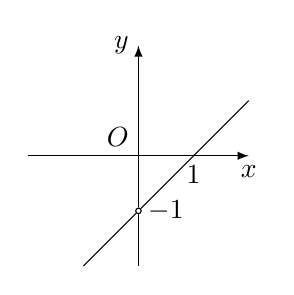
\begin{tikzpicture}[scale = 0.7,>=latex]
\draw [->] (-2,0) -- (2,0) node [below] {$x$};
\draw [->] (0,-2) -- (0,2) node [left] {$y$};
\draw (0,0) node [above left] {$O$};
\draw (1,0) node [below] {$1$} (0,-1) node [right] {$-1$};
\draw (-1,-2) -- (2,1);
\filldraw [white] (0,-1) circle (0.05);
\draw (0,-1) circle (0.05);
\end{tikzpicture}}{\begin{tikzpicture}[scale = 0.7,>=latex]
\draw [->] (-2,0) -- (2,0) node [below] {$x$};
\draw [->] (0,-2) -- (0,2) node [left] {$y$};
\draw (0,0) node [below right] {$O$};
\draw (1,0.1) -- (1,0) node [below] {$1$} (0,-1) node [right] {$-1$} (0,1) node [right] {$1$} (-1,0.1) -- (-1,0) node [below] {$-1$};
\draw (-1,-2) -- (0,-1) (0,1) -- (1,2);
\filldraw [white] (0,-1) circle (0.05);
\draw (0,-1) circle (0.05);
\filldraw [white] (0,1) circle (0.05);
\draw (0,1) circle (0.05);
\end{tikzpicture}}{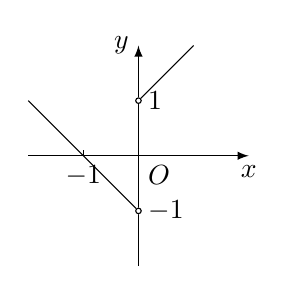
\begin{tikzpicture}[scale = 0.7,>=latex]
\draw [->] (-2,0) -- (2,0) node [below] {$x$};
\draw [->] (0,-2) -- (0,2) node [left] {$y$};
\draw (0,0) node [below right] {$O$};
\draw (0,-1) node [right] {$-1$} (0,1) node [right] {$1$} (-1,0.1) -- (-1,0) node [below] {$-1$};
\draw (-2,1) -- (0,-1) (0,1) -- (1,2);
\filldraw [white] (0,-1) circle (0.05);
\draw (0,-1) circle (0.05);
\filldraw [white] (0,1) circle (0.05);
\draw (0,1) circle (0.05);
\end{tikzpicture}}


关联目标:

暂未关联目标



标签: 第二单元

答案: 暂无答案

解答或提示: 暂无解答与提示

使用记录:

暂无使用记录


出处: 代数精编第三章函数
\item { (005304)}函数$y=\sqrt {1-x^2}+\sqrt {x+1}$的定义域为\blank{50}.


关联目标:

暂未关联目标



标签: 第二单元

答案: 暂无答案

解答或提示: 暂无解答与提示

使用记录:

暂无使用记录


出处: 代数精编第三章函数
\item { (005305)}函数$y=\dfrac 1{\sqrt {2x^2+3}}$的定义域为\blank{50}.


关联目标:

暂未关联目标



标签: 第二单元

答案: 暂无答案

解答或提示: 暂无解答与提示

使用记录:

暂无使用记录


出处: 代数精编第三章函数
\item { (005306)}函数$y=\dfrac{x+5}{3x^2-2x-1}$的定义域为\blank{50}.


关联目标:

暂未关联目标



标签: 第二单元

答案: 暂无答案

解答或提示: 暂无解答与提示

使用记录:

暂无使用记录


出处: 代数精编第三章函数
\item { (005307)}函数$y=\sqrt {6x-x^2-9}$的定义域为\blank{50}.


关联目标:

暂未关联目标



标签: 第二单元

答案: 暂无答案

解答或提示: 暂无解答与提示

使用记录:

暂无使用记录


出处: 代数精编第三章函数
\item { (005308)}函数$y=\sqrt {4-x^2}+\dfrac 1{|x|-1}$的定义域为\blank{50}.


关联目标:

暂未关联目标



标签: 第二单元

答案: 暂无答案

解答或提示: 暂无解答与提示

使用记录:

暂无使用记录


出处: 代数精编第三章函数
\item { (005309)}函数$y=\dfrac{x^3-1}{x+|x|}$的定义域为\blank{50}.


关联目标:

暂未关联目标



标签: 第二单元

答案: 暂无答案

解答或提示: 暂无解答与提示

使用记录:

暂无使用记录


出处: 代数精编第三章函数
\item { (005310)}函数$y=\dfrac 1{|x|-x^2}$的定义域为\blank{50}.


关联目标:

暂未关联目标



标签: 第二单元

答案: 暂无答案

解答或提示: 暂无解答与提示

使用记录:

暂无使用记录


出处: 代数精编第三章函数
\item { (005311)}函数$y=\sqrt {1-(\dfrac{x-1}{x+1})^2}$的定义域为\blank{50}.


关联目标:

暂未关联目标



标签: 第二单元

答案: 暂无答案

解答或提示: 暂无解答与提示

使用记录:

暂无使用记录


出处: 代数精编第三章函数
\item { (005312)}函数$y=\dfrac{\sqrt {x^2-2x-15}}{|x+3|-8}$的定义域为\blank{50}.


关联目标:

暂未关联目标



标签: 第二单元

答案: 暂无答案

解答或提示: 暂无解答与提示

使用记录:

暂无使用记录


出处: 代数精编第三章函数
\item { (005313)}函数$y=1-\dfrac 1{x+2}$的值域为\blank{50}.


关联目标:

暂未关联目标



标签: 第二单元

答案: 暂无答案

解答或提示: 暂无解答与提示

使用记录:

暂无使用记录


出处: 代数精编第三章函数
\item { (005314)}函数$y=\dfrac 3{2x}$的值域为\blank{50}.


关联目标:

暂未关联目标



标签: 第二单元

答案: 暂无答案

解答或提示: 暂无解答与提示

使用记录:

暂无使用记录


出处: 代数精编第三章函数
\item { (005315)}函数$y=\dfrac{x+3}{x-3}$的值域为\blank{50}.


关联目标:

暂未关联目标



标签: 第二单元

答案: 暂无答案

解答或提示: 暂无解答与提示

使用记录:

暂无使用记录


出处: 代数精编第三章函数
\item { (005316)}函数$y=\dfrac{5x+3}{x-3}$的值域为\blank{50}.


关联目标:

暂未关联目标



标签: 第二单元

答案: 暂无答案

解答或提示: 暂无解答与提示

使用记录:

暂无使用记录


出处: 代数精编第三章函数
\item { (005317)}函数$y=4+\sqrt {2x+1}$的值域为\blank{50}.


关联目标:

暂未关联目标



标签: 第二单元

答案: 暂无答案

解答或提示: 暂无解答与提示

使用记录:

暂无使用记录


出处: 代数精编第三章函数
\item { (005318)}函数$y=\sqrt {x-\dfrac 12x^2}$的值域为\blank{50}.


关联目标:

暂未关联目标



标签: 第二单元

答案: 暂无答案

解答或提示: 暂无解答与提示

使用记录:

暂无使用记录


出处: 代数精编第三章函数
\item { (005319)}函数$y=\sqrt {-x^2+x+2}$的值域为\blank{50}.


关联目标:

暂未关联目标



标签: 第二单元

答案: 暂无答案

解答或提示: 暂无解答与提示

使用记录:

暂无使用记录


出处: 代数精编第三章函数
\item { (005320)}函数$y=\dfrac{2x^2+2x+3}{x^2+x+1}$的值域为\blank{50}.


关联目标:

暂未关联目标



标签: 第二单元

答案: 暂无答案

解答或提示: 暂无解答与提示

使用记录:

暂无使用记录


出处: 代数精编第三章函数
\item { (005329)}若$-b<a<0$, 且函数$d(x)$的定义域是$[a,b]$, 则函数$F(x)=f(x)+f(-x)$的定义域是\bracket{20}.
\fourch{$[a,b]$}{$[-b,-a]$}{$[-b,b]$}{$[a,-a]$}


关联目标:

暂未关联目标



标签: 第二单元

答案: 暂无答案

解答或提示: 暂无解答与提示

使用记录:

暂无使用记录


出处: 代数精编第三章函数
\item { (005330)}若$f(x)$的定义域是$[ 0,1 ]$, 且$f(x+m)+f(x-m)$的定义域是$\varnothing$, 则正数$m$的取值范围是\bracket{20}.
\fourch{$0<m<1$}{$0<m\le \dfrac 12$}{$0<m<\dfrac 12$}{$m>\dfrac 12$}


关联目标:

暂未关联目标



标签: 第二单元

答案: 暂无答案

解答或提示: 暂无解答与提示

使用记录:

暂无使用记录


出处: 代数精编第三章函数
\item { (005331)}函数$y=\dfrac{x^2-1}{x^2+1}$的值域是\bracket{20}.
\fourch{$(-1,1)$}{$[-1,1]$}{$[-1,1)$}{$(-1,1]$}


关联目标:

暂未关联目标



标签: 第二单元

答案: 暂无答案

解答或提示: 暂无解答与提示

使用记录:

暂无使用记录


出处: 代数精编第三章函数
\item { (005333)}函数$f(x)=|1-x|-|x-3|(x\in \mathbf{R})$的值域是\bracket{20}.
\fourch{$[-2,2]$}{$[-1,3]$}{$[-3,1]$}{$[0,4]$}


关联目标:

暂未关联目标



标签: 第二单元

答案: 暂无答案

解答或提示: 暂无解答与提示

使用记录:

暂无使用记录


出处: 代数精编第三章函数
\item { (005334)}若函数$f(x)$的定义域是$[0,1]$, 分别求函数$f(1-2x)$和$f(x+a)$($a>0$)的定义域.


关联目标:

暂未关联目标



标签: 第二单元

答案: 暂无答案

解答或提示: 暂无解答与提示

使用记录:

暂无使用记录


出处: 代数精编第三章函数
\item { (005335)}若函数$f(x+1)$的定义域是$[-2,3)$, 求函数$f(\dfrac 1x+2)$的定义域.


关联目标:

暂未关联目标



标签: 第二单元

答案: 暂无答案

解答或提示: 暂无解答与提示

使用记录:

暂无使用记录


出处: 代数精编第三章函数
\item { (005336)}求函数$y=\dfrac{2x}{x^2+x+1}$的值域.


关联目标:

暂未关联目标



标签: 第二单元

答案: 暂无答案

解答或提示: 暂无解答与提示

使用记录:

暂无使用记录


出处: 代数精编第三章函数
\item { (005337)}求函数$y=\dfrac{x^2+x-1}{x^2+x+1}$的值域.


关联目标:

暂未关联目标



标签: 第二单元

答案: 暂无答案

解答或提示: 暂无解答与提示

使用记录:

暂无使用记录


出处: 代数精编第三章函数
\item { (005338)}求函数$y=\dfrac{x^2-1}{x^2-5x+4}$的值域.


关联目标:

暂未关联目标



标签: 第二单元

答案: 暂无答案

解答或提示: 暂无解答与提示

使用记录:

暂无使用记录


出处: 代数精编第三章函数
\item { (005341)}求函数$y=3x-2+\sqrt {3-2x}$的值域.


关联目标:

暂未关联目标



标签: 第二单元

答案: 暂无答案

解答或提示: 暂无解答与提示

使用记录:

暂无使用记录


出处: 代数精编第三章函数
\item { (005342)}求函数$y=2x+\sqrt {2x-1}$的值域.


关联目标:

暂未关联目标



标签: 第二单元

答案: 暂无答案

解答或提示: 暂无解答与提示

使用记录:

暂无使用记录


出处: 代数精编第三章函数
\item { (005343)}求函数$y=(x-1)(x-2)(x-3)(x-4)+15$的值域.


关联目标:

暂未关联目标



标签: 第二单元

答案: 暂无答案

解答或提示: 暂无解答与提示

使用记录:

暂无使用记录


出处: 代数精编第三章函数
\item { (005349)}已知函数$f(x)$的定义域是一切非零实数, 且满足$3f(x)+2f(\dfrac 1x)=4x$, 求, $f(x)$的表达式.


关联目标:

暂未关联目标



标签: 第二单元

答案: 暂无答案

解答或提示: 暂无解答与提示

使用记录:

暂无使用记录


出处: 代数精编第三章函数
\item { (005350)}作出函数$y=1+\dfrac{|x|}x$的图像.


关联目标:

暂未关联目标



标签: 第二单元

答案: 暂无答案

解答或提示: 暂无解答与提示

使用记录:

暂无使用记录


出处: 代数精编第三章函数
\item { (005351)}作出函数$y=x-|1-x|$的图像.


关联目标:

暂未关联目标



标签: 第二单元

答案: 暂无答案

解答或提示: 暂无解答与提示

使用记录:

暂无使用记录


出处: 代数精编第三章函数
\item { (005352)}作出函数$y=|x^2-4x+3|$的图像.


关联目标:

暂未关联目标



标签: 第二单元

答案: 暂无答案

解答或提示: 暂无解答与提示

使用记录:

暂无使用记录


出处: 代数精编第三章函数
\item { (005353)}作出函数$y=\dfrac{x^3+x}{|x|}$的图像.


关联目标:

暂未关联目标



标签: 第二单元

答案: 暂无答案

解答或提示: 暂无解答与提示

使用记录:

暂无使用记录


出处: 代数精编第三章函数
\item { (005354)}作出函数$y=\dfrac{(x+\dfrac 12)}{|x|-x}^0$的图像.


关联目标:

暂未关联目标



标签: 第二单元

答案: 暂无答案

解答或提示: 暂无解答与提示

使用记录:

暂无使用记录


出处: 代数精编第三章函数
\item { (005355)}已知$f(x)=-x^2+2x+3$, 画出函数$y=\dfrac 12[f(x)+|f(x)|]$的图像.


关联目标:

暂未关联目标



标签: 第二单元

答案: 暂无答案

解答或提示: 暂无解答与提示

使用记录:

暂无使用记录


出处: 代数精编第三章函数
\item { (005356)}已知$f(x)=|x|$, $x\in [-1,1]$, 作出函数$y=f(x+1)+1$的图像.


关联目标:

暂未关联目标



标签: 第二单元

答案: 暂无答案

解答或提示: 暂无解答与提示

使用记录:

暂无使用记录


出处: 代数精编第三章函数
\item { (005363)}画出函数$y=x^2-2|x|-1$的图像.


关联目标:

暂未关联目标



标签: 第二单元

答案: 暂无答案

解答或提示: 暂无解答与提示

使用记录:

暂无使用记录


出处: 代数精编第三章函数
\item { (005364)}求函数$y=\dfrac{x-2}{2x+1}$的值域.


关联目标:

暂未关联目标



标签: 第二单元

答案: 暂无答案

解答或提示: 暂无解答与提示

使用记录:

暂无使用记录


出处: 代数精编第三章函数
\item { (005365)}已知函数$f(x)=(x-1)^2$($x\le 1$), 又$f(x)$和$\varphi (x)$的图像关于直线$y=x$对称, 求$\varphi (x)$的表达式.


关联目标:

暂未关联目标



标签: 第二单元

答案: 暂无答案

解答或提示: 暂无解答与提示

使用记录:

暂无使用记录


出处: 代数精编第三章函数
\item { (005445)}已知幂函数$f(x)$的图像经过点$(2,\dfrac{\sqrt 2}2)$, 则$f(4)$的值等于\bracket{20}.
\fourch{$16$}{$\dfrac 1{16}$}{$\dfrac 12$}{$2$}


关联目标:

暂未关联目标



标签: 第二单元

答案: 暂无答案

解答或提示: 暂无解答与提示

使用记录:

暂无使用记录


出处: 代数精编第三章函数
\item { (005446)}下列幂函数中, 定义域为$\{x|x>0\}$的是\bracket{20}.
\fourch{$y=x^{\frac 23}$}{$y=x^{\frac 32}$}{$y=x^{-\frac 23}$}{$y=x^{-\frac 32}$}


关联目标:

暂未关联目标



标签: 第二单元

答案: 暂无答案

解答或提示: 暂无解答与提示

使用记录:

暂无使用记录


出处: 代数精编第三章函数
\item { (005447)}幂函数$y=x^n(n\in \mathbf{Z})$的图像一定不经过\bracket{20}.
\fourch{第一象限}{第二象限}{第三象限}{第四象限}


关联目标:

暂未关联目标



标签: 第二单元

答案: 暂无答案

解答或提示: 暂无解答与提示

使用记录:

暂无使用记录


出处: 代数精编第三章函数
\item { (005448)}函数$f(x)=x^{\frac 23}$的图像是\bracket{20}.
\fourch{\begin{tikzpicture}[scale = 0.7, >=latex]
\draw [->] (-2,0) -- (2,0) node [below] {$x$};
\draw [->] (0,-2) -- (0,2) node [left] {$y$};
\draw (0,0) node [below left] {$O$};
\draw (1,0.2) -- (1,0) node [below] {$1$};
\draw (0.2,1) -- (0,1) node [left] {$1$};
\draw [domain = 0:4,samples = 400] plot ({\x^(1/2)},{\x^(1/3)});
\end{tikzpicture}}{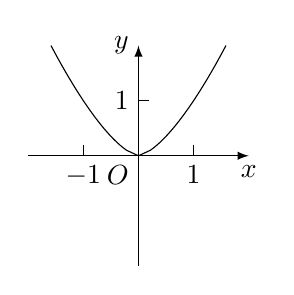
\begin{tikzpicture}[scale = 0.7, >=latex]
\draw [->] (-2,0) -- (2,0) node [below] {$x$};
\draw [->] (0,-2) -- (0,2) node [left] {$y$};
\draw (0,0) node [below left] {$O$};
\draw (1,0.2) -- (1,0) node [below] {$1$};
\draw (0.2,1) -- (0,1) node [left] {$1$};
\draw (-1,0.2) -- (-1,0) node [below] {$-1$};
\draw [domain = 0:4,samples = 400] plot ({\x^(1/3)},{\x^(1/2)});
\draw [domain = 0:4,samples = 400] plot ({-\x^(1/3)},{\x^(1/2)});
\end{tikzpicture}}{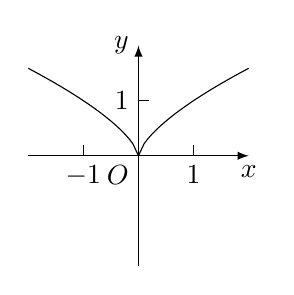
\begin{tikzpicture}[scale = 0.7, >=latex]
\draw [->] (-2,0) -- (2,0) node [below] {$x$};
\draw [->] (0,-2) -- (0,2) node [left] {$y$};
\draw (0,0) node [below left] {$O$};
\draw (1,0.2) -- (1,0) node [below] {$1$};
\draw (0.2,1) -- (0,1) node [left] {$1$};
\draw (-1,0.2) -- (-1,0) node [below] {$-1$};
\draw [domain = 0:4,samples = 400] plot ({\x^(1/2)},{\x^(1/3)});
\draw [domain = 0:4,samples = 400] plot ({-\x^(1/2)},{\x^(1/3)});
\end{tikzpicture}}{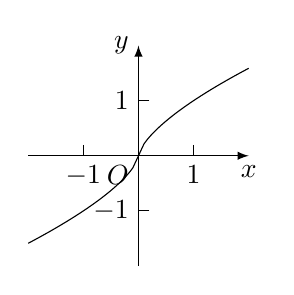
\begin{tikzpicture}[scale = 0.7, >=latex]
\draw [->] (-2,0) -- (2,0) node [below] {$x$};
\draw [->] (0,-2) -- (0,2) node [left] {$y$};
\draw (0,0) node [below left] {$O$};
\draw (1,0.2) -- (1,0) node [below] {$1$};
\draw (0.2,1) -- (0,1) node [left] {$1$};
\draw (-1,0.2) -- (-1,0) node [below] {$-1$};
\draw (0.2,-1) -- (0,-1) node [left] {$-1$};
\draw [domain = 0:4,samples = 400] plot ({\x^(1/2)},{\x^(1/3)});
\draw [domain = 0:4,samples = 400] plot ({-\x^(1/2)},{-\x^(1/3)});
\end{tikzpicture}}


关联目标:

暂未关联目标



标签: 第二单元

答案: 暂无答案

解答或提示: 暂无解答与提示

使用记录:

暂无使用记录


出处: 代数精编第三章函数
\item { (005449)}幂函数$y=x^m$和$y=x^n$在第一象限内的图像$C_1$和$C_2$图像所示, 则$m,n$之间的关系是\bracket{20}.
\begin{center}
    \begin{tikzpicture}[>=latex]
        \draw [->] (-1,0) -- (3,0) node [below] {$x$};
        \draw [->] (0,-1) -- (0,3) node [left] {$y$};
        \draw (0,0) node [below left] {$O$};
        \draw (1,0.2) -- (1,0) node [below] {$1$};
        \draw (0.2,1) -- (0,1) node [left] {$1$};
        \draw [domain = 0.5:2, samples = 400] plot (\x,{\x^(-5/4)});
        \draw [domain = 0.5:2, samples = 400] plot ({\x^(-5/4)},\x);
        \draw (0.5,{0.5^(-5/4)}) node [right] {$C_2$} ({0.5^(-5/4)},0.5) node [above] {$C_1$};
    \end{tikzpicture}
\end{center}
\fourch{$n<m<0$}{$m<n<0$}{$n>m>0$}{$m>n>0$}


关联目标:

暂未关联目标



标签: 第二单元

答案: 暂无答案

解答或提示: 暂无解答与提示

使用记录:

暂无使用记录


出处: 代数精编第三章函数
\item { (005450)}图中, $C_1,C_2,C_3$为幂函数$y=x^a$在第一象限的图像, 则解析式中的指数$\alpha$依次可以取\bracket{20}.
\begin{center}
    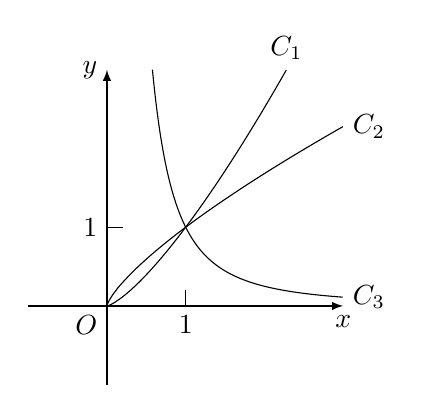
\begin{tikzpicture}[>=latex]
        \draw [->] (-1,0) -- (3,0) node [below] {$x$};
        \draw [->] (0,-1) -- (0,3) node [left] {$y$};
        \draw (0,0) node [below left] {$O$};
        \draw (1,0.2) -- (1,0) node [below] {$1$};
        \draw (0.2,1) -- (0,1) node [left] {$1$};
        \draw [domain = {sqrt(3)/3}:3, samples = 400] plot (\x,{\x^(-2)});
        \draw [domain = 0:3, samples = 400] plot (\x,{\x^(3/4)});
        \draw [domain = 0:{3^(3/4)}, samples = 400] plot (\x,{\x^(4/3)});
        \draw (3,{1/9}) node [right] {$C_3$} (3,{3^(3/4)}) node [right] {$C_2$} ({3^(3/4)},3) node [above] {$C_1$};
    \end{tikzpicture}
\end{center}
\fourch{$\dfrac 43,-2,\dfrac 34$}{$-2,\dfrac 34,\dfrac 43$}{$-2,\dfrac 43,\dfrac 34$}{$\dfrac 34,\dfrac 43,-2$}


关联目标:

暂未关联目标



标签: 第二单元

答案: 暂无答案

解答或提示: 暂无解答与提示

使用记录:

暂无使用记录


出处: 代数精编第三章函数
\item { (005451)}函数$y=x^{\frac 56}$的定义域为\blank{50}, 值域为\blank{50}.


关联目标:

暂未关联目标



标签: 第二单元

答案: 暂无答案

解答或提示: 暂无解答与提示

使用记录:

暂无使用记录


出处: 代数精编第三章函数
\item { (005452)}函数$y=x^{\frac 35}$的定义域为\blank{50}, 值域为\blank{50}.


关联目标:

暂未关联目标



标签: 第二单元

答案: 暂无答案

解答或提示: 暂无解答与提示

使用记录:

暂无使用记录


出处: 代数精编第三章函数
\item { (005453)}函数$y=x^{\frac 85}$的定义域为\blank{50}, 值域为\blank{50}.


关联目标:

暂未关联目标



标签: 第二单元

答案: 暂无答案

解答或提示: 暂无解答与提示

使用记录:

暂无使用记录


出处: 代数精编第三章函数
\item { (005454)}函数$y=x^{-\frac 54}$的定义域为\blank{50}, 值域为\blank{50}.


关联目标:

暂未关联目标



标签: 第二单元

答案: 暂无答案

解答或提示: 暂无解答与提示

使用记录:

暂无使用记录


出处: 代数精编第三章函数
\item { (005455)}函数$y=x^{-\frac 53}$的定义域为\blank{50}, 值域为\blank{50}.


关联目标:

暂未关联目标



标签: 第二单元

答案: 暂无答案

解答或提示: 暂无解答与提示

使用记录:

暂无使用记录


出处: 代数精编第三章函数
\item { (005456)}函数$y=x^{-\frac 23}$的定义域为\blank{50}, 值域为\blank{50}.


关联目标:

暂未关联目标



标签: 第二单元

答案: 暂无答案

解答或提示: 暂无解答与提示

使用记录:

暂无使用记录


出处: 代数精编第三章函数
\item { (005457)}函数$y=-2(x+5)^{-\frac 14}$的定义域为\blank{50}, 值域为\blank{50}.


关联目标:

暂未关联目标



标签: 第二单元

答案: 暂无答案

解答或提示: 暂无解答与提示

使用记录:

暂无使用记录


出处: 代数精编第三章函数
\item { (005458)}函数$y=5(2x-1)^{\frac 34}$的定义域为\blank{50}, 值域为\blank{50}.


关联目标:

暂未关联目标



标签: 第二单元

答案: 暂无答案

解答或提示: 暂无解答与提示

使用记录:

暂无使用记录


出处: 代数精编第三章函数
\item { (005459)}将下列函数图像的标号, 填在相应函数后面的横线上:\\
(1) $y=x^{\frac 23}$:\blank{50}; (2) $y=x^{-2}$:\blank{50}; (3) $y=x^{\frac 12}$:\blank{50};\\
(4) $y=x^{-1}$:\blank{50}; (5) $y=x^{\frac 13}$:\blank{50}; (6)$y=x^{\frac 32}$:\blank{50};\\ (7)$y=x^{\frac 43}$:\blank{50}; (8)$y=x^{-\frac 12}$:\blank{50}; (9)$y=x^{\frac 53}$:\blank{50}.
\begin{center}
    \begin{tikzpicture}[>=latex,scale = 0.6]
        \draw [->] (-2.5,0) -- (2.5,0) node [below] {$x$};
        \draw [->] (0,-2.5) -- (0,2.5) node [left] {$y$};
        \draw (0,0) node [below left] {$O$};
        \draw (0.2,1) -- (0,1) node [left] {$1$} (0.2,-1) -- (0,-1) node [left] {$-1$};
        \draw (1,0.2) -- (1,0) node [below] {$1$} (-1,0.2) -- (-1,0) node [below] {$1$};
        \draw (0,-2.5) node [below] {(A)};
        \draw [domain = 0:2.4, samples = 400] plot (\x,{\x^(1/2)});
    \end{tikzpicture}
    \begin{tikzpicture}[>=latex,scale = 0.6]
        \draw [->] (-2.5,0) -- (2.5,0) node [below] {$x$};
        \draw [->] (0,-2.5) -- (0,2.5) node [left] {$y$};
        \draw (0,0) node [below left] {$O$};
        \draw (0,-2.5) node [below] {(B)};
        \draw (0.2,1) -- (0,1) node [left] {$1$} (0.2,-1) -- (0,-1) node [left] {$-1$};
        \draw (1,0.2) -- (1,0) node [below] {$1$} (-1,0.2) -- (-1,0) node [below] {$1$};
        \draw [domain = 0:2.4, samples = 400] plot (\x,{\x^(1/3)});
        \draw [domain = 0:2.4, samples = 400] plot (-\x,{-\x^(1/3)});
    \end{tikzpicture}
    \begin{tikzpicture}[>=latex,scale = 0.6]
        \draw [->] (-2.5,0) -- (2.5,0) node [below] {$x$};
        \draw [->] (0,-2.5) -- (0,2.5) node [left] {$y$};
        \draw (0,0) node [below left] {$O$};
        \draw (0,-2.5) node [below] {(C)};
        \draw (0.2,1) -- (0,1) node [left] {$1$} (0.2,-1) -- (0,-1) node [left] {$-1$};
        \draw (1,0.2) -- (1,0) node [below] {$1$} (-1,0.2) -- (-1,0) node [below] {$1$};
        \draw [domain = {1/sqrt(2.4)}:2.4, samples = 400] plot (\x,{\x^(-2)});
        \draw [domain = {1/sqrt(2.4)}:2.4, samples = 400] plot (-\x,{\x^(-2)});
    \end{tikzpicture}\\
    \begin{tikzpicture}[>=latex,scale = 0.6]
        \draw [->] (-2.5,0) -- (2.5,0) node [below] {$x$};
        \draw [->] (0,-2.5) -- (0,2.5) node [left] {$y$};
        \draw (0,0) node [below left] {$O$};
        \draw (0,-2.5) node [below] {(D)};
        \draw (0.2,1) -- (0,1) node [left] {$1$} (0.2,-1) -- (0,-1) node [left] {$-1$};
        \draw (1,0.2) -- (1,0) node [below] {$1$} (-1,0.2) -- (-1,0) node [below] {$1$};
        \draw [domain = 0:{2.4^(3/4)}, samples = 400] plot (\x,{\x^(4/3)});
        \draw [domain = 0:{2.4^(3/4)}, samples = 400] plot (-\x,{\x^(4/3)});
    \end{tikzpicture}
    \begin{tikzpicture}[>=latex,scale = 0.6]
        \draw [->] (-2.5,0) -- (2.5,0) node [below] {$x$};
        \draw [->] (0,-2.5) -- (0,2.5) node [left] {$y$};
        \draw (0,0) node [below left] {$O$};
        \draw (0,-2.5) node [below] {(E)};
        \draw (0.2,1) -- (0,1) node [left] {$1$} (0.2,-1) -- (0,-1) node [left] {$-1$};
        \draw (1,0.2) -- (1,0) node [below] {$1$} (-1,0.2) -- (-1,0) node [below] {$1$};
        \draw [domain = 0:2.4, samples = 400] plot (\x,{\x^(2/3)});
        \draw [domain = 0:2.4, samples = 400] plot (-\x,{\x^(2/3)});
    \end{tikzpicture}
    \begin{tikzpicture}[>=latex,scale = 0.6]
        \draw [->] (-2.5,0) -- (2.5,0) node [below] {$x$};
        \draw [->] (0,-2.5) -- (0,2.5) node [left] {$y$};
        \draw (0,0) node [below left] {$O$};
        \draw (0,-2.5) node [below] {(F)};
        \draw (0.2,1) -- (0,1) node [left] {$1$} (0.2,-1) -- (0,-1) node [left] {$-1$};
        \draw (1,0.2) -- (1,0) node [below] {$1$} (-1,0.2) -- (-1,0) node [below] {$1$};
        \draw [domain = 0:{2.4^(3/5)}, samples = 400] plot (\x,{\x^(5/3)});
        \draw [domain = 0:{2.4^(3/5)}, samples = 400] plot (-\x,{-\x^(5/3)});
    \end{tikzpicture}\\
    \begin{tikzpicture}[>=latex,scale = 0.6]
        \draw [->] (-2.5,0) -- (2.5,0) node [below] {$x$};
        \draw [->] (0,-2.5) -- (0,2.5) node [left] {$y$};
        \draw (0,0) node [below left] {$O$};
        \draw (0,-2.5) node [below] {(G)};
        \draw (0.2,1) -- (0,1) node [left] {$1$} (0.2,-1) -- (0,-1) node [left] {$-1$};
        \draw (1,0.2) -- (1,0) node [below] {$1$} (-1,0.2) -- (-1,0) node [below] {$1$};
        \draw [domain = {1/2.4}:2.4] plot (\x,{1/\x});
        \draw [domain = {1/2.4}:2.4] plot (-\x,{-1/\x});
    \end{tikzpicture}
    \begin{tikzpicture}[>=latex,scale = 0.6]
        \draw [->] (-2.5,0) -- (2.5,0) node [below] {$x$};
        \draw [->] (0,-2.5) -- (0,2.5) node [left] {$y$};
        \draw (0,0) node [below left] {$O$};
        \draw (0,-2.5) node [below] {(H)};
        \draw (0.2,1) -- (0,1) node [left] {$1$} (0.2,-1) -- (0,-1) node [left] {$-1$};
        \draw (1,0.2) -- (1,0) node [below] {$1$} (-1,0.2) -- (-1,0) node [below] {$1$};
        \draw [domain = {1/2.4^2}:2.4] plot (\x,{1/\x^(1/2)});
    \end{tikzpicture}
    \begin{tikzpicture}[>=latex,scale = 0.6]
        \draw [->] (-2.5,0) -- (2.5,0) node [below] {$x$};
        \draw [->] (0,-2.5) -- (0,2.5) node [left] {$y$};
        \draw (0,0) node [below left] {$O$};
        \draw (0,-2.5) node [below] {(I)};
        \draw (0.2,1) -- (0,1) node [left] {$1$} (0.2,-1) -- (0,-1) node [left] {$-1$};
        \draw (1,0.2) -- (1,0) node [below] {$1$} (-1,0.2) -- (-1,0) node [below] {$1$};
        \draw [domain = 0:{2.4^(2/3)}] plot (\x,{\x^(3/2)});
    \end{tikzpicture}
\end{center}


关联目标:

暂未关联目标



标签: 第二单元

答案: 暂无答案

解答或提示: 暂无解答与提示

使用记录:

暂无使用记录


出处: 代数精编第三章函数
\item { (005460)}若幂函数$y=x^n$的图像在$0<x<1$时位于直线$y=x$的下方, 则$n$的取值范围是\blank{50}.


关联目标:

暂未关联目标



标签: 第二单元

答案: 暂无答案

解答或提示: 暂无解答与提示

使用记录:

暂无使用记录


出处: 代数精编第三章函数
\item { (005461)}若幂函数$y=x^n$的图像在$0<x<1$时位于直线$y=x$的上方, 则$n$的取值范围是\blank{50}.


关联目标:

暂未关联目标



标签: 第二单元

答案: 暂无答案

解答或提示: 暂无解答与提示

使用记录:

暂无使用记录


出处: 代数精编第三章函数
\item { (005462)}函数$f(x)=x^{k^2-2k-3}$($k\in \mathbf{Z}$)的图像如图所示, 则$k=$\blank{50}.
\begin{center}
    \begin{tikzpicture}[>=latex]
        \draw [->] (-2.5,0) -- (2.5,0) node [below] {$x$};
        \draw [->] (0,-0.5) -- (0,2.5) node [left] {$y$};
        \draw (0,0) node [below left] {$O$};
        \draw (0,-0.5) node [below] {(C)};
        \draw (0.2,1) -- (0,1) node [left] {$1$};
        \draw (1,0.2) -- (1,0) node [below] {$1$} (-1,0.2) -- (-1,0) node [below] {$1$};
        \draw [domain = {1/2.4^(1/4)}:2.4, samples = 400] plot (\x,{\x^(-4)});
        \draw [domain = {1/2.4^(1/4)}:2.4, samples = 400] plot (-\x,{\x^(-4)});
    \end{tikzpicture}
\end{center}


关联目标:

暂未关联目标



标签: 第二单元

答案: 暂无答案

解答或提示: 暂无解答与提示

使用记录:

暂无使用记录


出处: 代数精编第三章函数
\item { (005463)}幂函数$y=x^p$与$y=x^q$的图像都通过定点\blank{50}, 它们在第一象限部分关于直线$y=x$对称, 则$p,q$应满足的条件是\blank{50}.


关联目标:

K0207004B|D02002B|会用图像上任意一点关于原点(或关于$y$轴)的对称点仍落在图像上证明函数的图像关于原点(或$y$轴)对称.

K0208003B|D02002B|知道幂函数的图像过定点$(1,1)$.



标签: 第二单元

答案: 暂无答案

解答或提示: 暂无解答与提示

使用记录:

暂无使用记录


出处: 代数精编第三章函数
\item { (005471)}已知函数$y=x^{n^2-2n-3}$($n\in \mathbf{Z}$)的图像与两坐标轴都无公共点, 且其图像关于$y$轴对称, 求$n$的值, 并画出相应的函数图像.


关联目标:

暂未关联目标



标签: 第二单元

答案: 暂无答案

解答或提示: 暂无解答与提示

使用记录:

暂无使用记录


出处: 代数精编第三章函数
\item { (005477)}若函数$f(x)$在定义域$\mathbf{R}$上为增函数, 且$f(x)<0$, 则下列函数在$\mathbf{R}$上为增函数的是\bracket{20}.
\fourch{$y=|f(x)|$}{$y=\dfrac 1{f(x)}$}{$y=[ f(x) ]^2$}{$y=[ f(x) ]^3$}


关联目标:

暂未关联目标



标签: 第二单元

答案: 暂无答案

解答或提示: 暂无解答与提示

使用记录:

暂无使用记录


出处: 代数精编第三章函数
\item { (005484)}已知$f(x)=-x^3-x+1$($x\in \mathbf{R}$), 求证$y=f(x)$在定义域上为减函数.


关联目标:

暂未关联目标



标签: 第二单元

答案: 暂无答案

解答或提示: 暂无解答与提示

使用记录:

暂无使用记录


出处: 代数精编第三章函数
\item { (005486)}求证: $f(x)=\sqrt x-\dfrac 1x$在定义域上是增函数.


关联目标:

暂未关联目标



标签: 第二单元

答案: 暂无答案

解答或提示: 暂无解答与提示

使用记录:

暂无使用记录


出处: 代数精编第三章函数
\item { (005493)}下列函数中既是奇函数, 又在定义域上为增函数的是\bracket{20}.
\fourch{$f(x)=3x+1$}{$f(x)=\dfrac 1x$}{$f(x)=1-\dfrac 1x$}{$f(x)=x^3$}


关联目标:

暂未关联目标



标签: 第二单元

答案: 暂无答案

解答或提示: 暂无解答与提示

使用记录:

暂无使用记录


出处: 代数精编第三章函数
\item { (005496)}已知$f(x)$是奇函数, 则下列各点中在函数$y=f(x)$的图像上的点的是\bracket{20}.
\fourch{$(a,f(-a))$}{$(-a,-f(a))$}{$(\dfrac 1a,-f(\dfrac 1a))$}{$(-\sin a,-f(-\sin a))$}


关联目标:

暂未关联目标



标签: 第二单元

答案: 暂无答案

解答或提示: 暂无解答与提示

使用记录:

暂无使用记录


出处: 代数精编第三章函数
\item { (005498)}若奇函数$f(x)$的定义域是$\mathbf{R}$, 则$f(0)=$\blank{50}.


关联目标:

暂未关联目标



标签: 第二单元

答案: 暂无答案

解答或提示: 暂无解答与提示

使用记录:

暂无使用记录


出处: 代数精编第三章函数
\item { (005505)}若函数$y=f(x)$是偶函数, 其图像与$x$轴有四个交点, 则方程$f(x)=0$的所有实数根之和为\bracket{20}.
\fourch{$4$}{$2$}{$1$}{$0$}


关联目标:

暂未关联目标



标签: 第二单元

答案: 暂无答案

解答或提示: 暂无解答与提示

使用记录:

暂无使用记录


出处: 代数精编第三章函数
\item { (005508)}$f(x)+f(2-x)+2=0$对任何实数$x$都成立, 则$f(x)$的图像\bracket{20}.
\twoch{关于直线$x=1$成轴对称图形}{关于直线$x=2$成轴对称图形}{关于点$(1, -1)$成中心对称图形}{关于点$(-1,1)$成中心对称图形}


关联目标:

暂未关联目标



标签: 第二单元

答案: 暂无答案

解答或提示: 暂无解答与提示

使用记录:

暂无使用记录


出处: 代数精编第三章函数
\item { (005519)}已知奇函数$f(x)$在定义域$(-l, l)$上是减函数, 求满足$f(1-m)+f(1-m^2)<0$的实数$m$的取值范围.


关联目标:

暂未关联目标



标签: 第二单元

答案: 暂无答案

解答或提示: 暂无解答与提示

使用记录:

暂无使用记录


出处: 代数精编第三章函数
\item { (005522)}求证: 定义域为$(-l,l)$的任何函数都能表示成一个奇函数与一个偶函数之和.


关联目标:

暂未关联目标



标签: 第二单元

答案: 暂无答案

解答或提示: 暂无解答与提示

使用记录:

暂无使用记录


出处: 代数精编第三章函数
\item { (005524)}函数$y=\sqrt {x^2-2x+3}$($x\le 1$)的反函数的定义域是\bracket{20}.
\fourch{$[0,+\infty)$}{$(2,+\infty)$}{$(-\infty ,1]$}{$[\sqrt 2,+\infty)$}


关联目标:

暂未关联目标



标签: 第二单元

答案: 暂无答案

解答或提示: 暂无解答与提示

使用记录:

暂无使用记录


出处: 代数精编第三章函数
\item { (005527)}若函数$y=g(x)$的图像与函数$f(x)=(x-1)^2$($x\le 1$)的图像关于直线$y=x$对称.则$g(x)$的表达式是\bracket{20}.
\twoch{$g(x)=1-\sqrt x$($x\ge 0$)}{$g(x)=1+\sqrt x$($x\ge 0$)}{$g(x)=\sqrt {1-x}$($x\le 1$)}{$g(x)=\sqrt {1+x}$($x\ge -1$)}


关联目标:

暂未关联目标



标签: 第二单元

答案: 暂无答案

解答或提示: 暂无解答与提示

使用记录:

暂无使用记录


出处: 代数精编第三章函数
\item { (005530)}若函数$f(x)$的图像经过点$(0, -1)$, 则函数$f(x+4)$的反函数的图像必经过点\bracket{20}.
\fourch{$(—1,4)$}{$(-4,-1)$}{$(-1,-4)$}{$(1,-4)$}


关联目标:

暂未关联目标



标签: 第二单元

答案: 暂无答案

解答或提示: 暂无解答与提示

使用记录:

暂无使用记录


出处: 代数精编第三章函数
\item { (005531)}已知函数$y=-\sqrt {1-x^2}$的反函数是$y=-\sqrt {1-x^2}$, 则原函数的定义域``最大''可以是\blank{50}.


关联目标:

暂未关联目标



标签: 第二单元

答案: 暂无答案

解答或提示: 暂无解答与提示

使用记录:

暂无使用记录


出处: 代数精编第三章函数
\item { (005533)}若点$(1, 2)$既在函数$y=\sqrt {ax+b}$的图像上.又在其反函数的图像上, 则$a=$\blank{50}, $b=$\blank{50}.


关联目标:

暂未关联目标



标签: 第二单元

答案: 暂无答案

解答或提示: 暂无解答与提示

使用记录:

暂无使用记录


出处: 代数精编第三章函数
\item { (005542)}若函数$y=\sqrt {x-m}$与其反函数的图像有公共点, 则$m$的取值范围是\bracket{20}.
\fourch{$m\ge \dfrac 14$}{$m\le \dfrac 14$}{$m\ge 0$}{$m\le 0$}


关联目标:

暂未关联目标



标签: 第二单元

答案: 暂无答案

解答或提示: 暂无解答与提示

使用记录:

暂无使用记录


出处: 代数精编第三章函数
\item { (005543)}已知$y=g(x)$是函数$y=f(x)$的反函数, 又$y=h(x)$与$y=g(x)$的图像关于原点$O(0,0)$对称, 则$h(x)$的表达式是\bracket{20}.
\fourch{$y=f^{-1}(x)$}{$y=-f^{-1}(x)$}{$y=f^{-1}(-x)$}{$y=-f^{-1}(-x)$}


关联目标:

暂未关联目标



标签: 第二单元

答案: 暂无答案

解答或提示: 暂无解答与提示

使用记录:

暂无使用记录


出处: 代数精编第三章函数
\item { (005547)}已知定义域为$(-\infty ,0]$的函数$f(x)$满足$f(x-1)=x^2-2x$, 则$f^{-1}(-\dfrac 12)=$\blank{50}.


关联目标:

暂未关联目标



标签: 第二单元

答案: 暂无答案

解答或提示: 暂无解答与提示

使用记录:

暂无使用记录


出处: 代数精编第三章函数
\item { (005548)}求函数$f(x)=\begin{cases}
   x+1, &  x>0,  \\ x-1, &  x<0  \end{cases}$的反函数, 并作出其反函数的图像.


关联目标:

暂未关联目标



标签: 第二单元

答案: 暂无答案

解答或提示: 暂无解答与提示

使用记录:

暂无使用记录


出处: 代数精编第三章函数
\item { (005549)}已知函数$f(x)=x^2+2x+1$.\\
(1) 若函数的定义域是$(-\infty ,+\infty)$, 这个函数有没有反函数?\\
(2) 若函数的定义域是$[0,+\infty)$, 求其反函数;\\
(3) 若函数的定义域是$(-\infty ,-1]$, 求其反函数.


关联目标:

暂未关联目标



标签: 第二单元

答案: 暂无答案

解答或提示: 暂无解答与提示

使用记录:

暂无使用记录


出处: 代数精编第三章函数
\item { (005562)}已知函数$f(x)=2x+1$, $g(x)=1.5^x$, $h(x)=x^{1.5}$, 试用数值计算比较三个函数在$[0,+\infty)$上的函数值的大小、图像递增的快慢. 并说明在函数图像上的表现.
解  列表并计算得:
\begin{center}
    \begin{longtable}{|c|c|c|c|c|c|c|}
        \hline
        $x$	 & $f(x)=2x+1$ & $f(x)-f(x-1)$ & $g(x)=1.5^x$ & $g(x)-g(x-1)$ & $h(x)=x^{1.5}$ & $h(x)-h(x-1)$ \\ \hline
        \endhead
        $0$ & $1$ & & $1$ & & $0$ &  \\ \hline
        $1$ & $3$ & $2$ & $1.5$ & $0.5$ & $1$ & $1$\\ \hline
        $2$ & $5$ & $2$ & $2.25$ & $0.75$ & $2.82842712$ & $1.82842712$\\ \hline
        $3$ & $7$ & $2$ & $3.375$ & $1.125$ & $5.19615242$ & $2.3677253$\\ \hline
        $4$ & $9$ & $2$ & $5.0625$ & $1.6875$ & $8$ & $2.80384758$\\ \hline
        $5$ & $11$ & $2$ & $7.59375$ & $2.53125$ & $11.1803399$ & $3.18033989$\\ \hline
        $6$ & $13$ & $2$ & $11.390625$ & $3.796875$ & $14.6969385$ & $3.51659857$\\ \hline
        $7$ & $15$ & $2$ & $17.085938$ & $5.6953125$ & $18.5202592$ & $3.82332072$\\ \hline
        $8$ & $17$ & $2$ & $25.628906$ & $8.5429688$ & $22.627417$ & $4.10715782$\\ \hline
        $9$ & $19$ & $2$ & $38.443359$ & $12.814453$ & $27$ & $4.372583$\\ \hline
        $10$ & $21$ & $2$ & $57.665039$ & $19.22168$ & $31.6227766$ & $4.6227766$\\ \hline
        $11$ & $23$ & $2$ & $86.497559$ & $28.83252$ & $36.4828727$ & $4.86009609$\\ \hline
        $12$ & $25$ & $2$ & $129.74634$ & $43.248779$ & $41.5692194$ & $5.08634669$\\ \hline
        $13$ & $27$ & $2$ & $194.61951$ & $64.873169$ & $46.8721666$ & $5.3029472$\\ \hline
        $14$ & $29$ & $2$ & $291.92926$ & $97.309753$ & $52.3832034$ & $5.51103683$\\ \hline
        $15$ & $31$ & $2$ & $437.89389$ & $145.96463$ & $58.0947502$ & $5.71154678$\\ \hline
        $16$ & $33$ & $2$ & $656.84084$ & $218.94695$ & $64$ & $5.90524981$\\ \hline
        $17$ & $35$ & $2$ & $985.26125$ & $328.42042$ & $70.0927956$ & $6.09279564$\\ \hline
        $18$ & $37$ & $2$ & $1477.8919$ & $492.63063$ & $76.3675324$ & $6.27473673$\\ \hline
        $19$ & $39$ & $2$ & $2216.8378$ & $738.94594$ & $82.8190799$ & $6.45154756$\\ \hline
        $20$ & $41$ & $2$ & $3325.2567$ & $1108.4189$ & $89.4427191$ & $6.62363917$\\ \hline
        $21$ & $43$ & $2$ & $4987.8851$ & $1662.6284$ & $96.2340896$ & $6.79137049$\\ \hline
        $22$ & $45$ & $2$ & $7481.8276$ & $2493.9425$ & $103.189147$ & $6.95505712$\\ \hline
        $23$ & $47$ & $2$ & $11222.741$ & $3740.9138$ & $110.304125$ & $7.11497832$\\ \hline
        $24$ & $49$ & $2$ & $16834.112$ & $5611.3707$ & $117.575508$ & $7.27138262$\\ \hline
        $25$ & $51$ & $2$ & $25251.168$ & $8417.0561$ & $125$ & $7.42449235$\\ \hline
        $26$ & $53$ & $2$ & $37876.752$ & $12625.584$ & $132.574507$ & $7.57450735$\\ \hline
        $27$ & $55$ & $2$ & $56815.129$ & $18938.376$ & $140.296115$ & $7.72160806$\\ \hline
        $28$ & $57$ & $2$ & $85222.693$ & $28407.564$ & $148.162073$ & $7.86595801$\\ \hline
        $29$ & $59$ & $2$ & $127834.04$ & $42611.346$ & $156.169779$ & $8.00770599$\\ \hline
        $30$ & $61$ & $2$ & $191751.06$ & $63917.02$ & $164.316767$ & $8.14698784$\\ \hline
        $\cdots$ & $\cdots$ & $\cdots$ & $\cdots$ & $\cdots$ & $\cdots$ & $\cdots$ \\ \hline
    \end{longtable}
\end{center}
得点$A,B,C,D$的横坐标分别约为$1.5,4.8, 6.5, 7.4$, 记作$x_A,x_B,x_C,x_D$.\\
(1) 三个函数的函数值的大小情况如下:\\
\textcircled{1} 当$0<x<x_A$时, $f(x)>g(x)>h(x)$;
\textcircled{2} 当$x_A<x<x_B$时, $f(x)>h(x)>g(x)$;
\textcircled{3} 由$x_B<x<x_C$时, $h(x)>f(x)>g(x)$;
\textcircled{4} 当$x_C<x<x_D$时, $h(x)>g(x)>f(x)$;
\textcircled{5} 当$x_D<x$时, $g(x)>h(x)>f(x)$;
\textcircled{6} 当$x=x_A$时, $f(x)>g(x)=h(x)$;
\textcircled{7} 当$x=x_B$时, $f(x)=h(x)>g(x)$;
\textcircled{8} 当$x=x_C$时, $f(x)=g(x)<h(x)$;
\textcircled{9} 当$x=x_D$时, $f(x)<g(x)=g(x)$.\\
(2) 它们在同一个平面直角坐标系下的图像如图14所示.
\begin{center}
    \begin{tikzpicture}[>=latex]
        \draw [->] (-0.1,0) -- (5,0) node [below] {$x$};
        \draw [->] (0,-0.1) -- (0,5.75) node [left] {$y$};
        \draw (0,0) node [below left] {$O$};
        \draw [domain = 0:9,samples = 100, name path = firstorder] plot ({\x/2},{(2*\x+1)/4});
        \draw (4.5,{19/4}) node [right] {$y=f(x)$};
        \draw [domain = 0:7.8, samples = 100, name path = exponential] plot ({\x/2},{1.5^(\x)/4}); 
        \draw (3.9,{1.5^7.8/4}) node [above right] {$y=g(x)$};
        \draw [domain = 0:8, samples = 100, name path = power] plot ({\x/2},{\x^(3/2)/4});
        \draw (4,{8^(3/2)/4}) node [below right] {$y=h(x)$};
        \path [name intersections = {of = firstorder and exponential, by = {T,C}}];
        \path [name intersections = {of = firstorder and power, by = B}];
        \path [name intersections = {of = exponential and power, by = {A,D}}];
        \filldraw (A) circle (0.05) node [below right] {$A$};
        \filldraw (B) circle (0.05) node [below right] {$B$};
        \filldraw (C) circle (0.05) node [below right] {$C$};
        \filldraw (D) circle (0.05) node [below right] {$D$};
        \foreach \i in {1,2,...,9}{\draw (\i/2,0.1) -- (\i/2,0) node [below] {$\i$};};
        \foreach \i in {1,3,...,21}{\draw (0.1,\i/4) -- (0,\i/4) node [left] {$\i$};};
    \end{tikzpicture}
\end{center}
由表格及图像可看出, 三个函数的函数值变化及相应增量规律为: 随着$x$的增大, 直线型均匀上升, 增量恒定; 指数型急剧上升, 在区间$[0,+\infty)$上递增增量快速增大; 幂函数型虽上升较快, 但随着$x$的不断增大上升趋势远不如指数型, 几乎微不足道, 其增量缓慢递增.


关联目标:

暂未关联目标



标签: 第二单元

答案: 暂无答案

解答或提示: 暂无解答与提示

使用记录:

暂无使用记录


出处: 代数精编第三章函数
\item { (005563)}已知函数$f(x)=4+a^{x-1}$的图像恒过记点$P$, 则点$P$的坐标是\bracket{20}.
\fourch{$(1, 5)$}{$(1, 4)$}{$(0, 4)$}{$(4, 0)$}


关联目标:

暂未关联目标



标签: 第二单元

答案: 暂无答案

解答或提示: 暂无解答与提示

使用记录:

暂无使用记录


出处: 代数精编第三章函数
\item { (005564)}下列函数中, 值域为$(0,+\infty)$的函数是\bracket{20}.
\fourch{$y=(\dfrac 18)^{2-x}$}{$y=\sqrt {1-3^x}$}{$y=\sqrt {(\dfrac 13)^x-1}$}{$y=2^{\frac 1{3-x}}$}


关联目标:

暂未关联目标



标签: 第二单元

答案: 暂无答案

解答或提示: 暂无解答与提示

使用记录:

暂无使用记录


出处: 代数精编第三章函数
\item { (005569)}在同一平面直角坐标系中, 函数$f(x)=ax$与$g(x)=a^x$的图像可能是\bracket{20}.
\fourch{\begin{tikzpicture}[scale = 0.15, >=latex]
    \draw [->] (-8,0) -- (8,0) node [below] {$x$};
    \draw [->] (0,-4) -- (0,12) node [left] {$y$};
    \draw (0,0) node [below left] {$O$};
    \draw [domain = -6:2, samples = 100] plot (\x,{-1.5*\x});
    \draw [domain = -6:6, samples = 100] plot (\x,{1.5^\x});
\end{tikzpicture}}{\begin{tikzpicture}[scale = 0.15, >=latex]
    \draw [->] (-8,0) -- (8,0) node [below] {$x$};
    \draw [->] (0,-4) -- (0,12) node [left] {$y$};
    \draw (0,0) node [below left] {$O$};
    \draw [domain = -2:6, samples = 100] plot (\x,{1.5*\x});
    \draw [domain = -6:6, samples = 100] plot (-\x,{1.5^\x});
\end{tikzpicture}}{\begin{tikzpicture}[scale = 0.15, >=latex]
    \draw [->] (-8,0) -- (8,0) node [below] {$x$};
    \draw [->] (0,-4) -- (0,12) node [left] {$y$};
    \draw (0,0) node [below left] {$O$};
    \draw [domain = -2:6, samples = 100] plot (\x,{1.5*\x});
    \draw [domain = -6:6, samples = 100] plot (\x,{1.5^\x});
\end{tikzpicture}}{\begin{tikzpicture}[scale = 0.15, >=latex]
    \draw [->] (-8,0) -- (8,0) node [below] {$x$};
    \draw [->] (0,-4) -- (0,12) node [left] {$y$};
    \draw (0,0) node [below left] {$O$};
    \draw [domain = -2:6, samples = 100] plot (-\x,{1.5*\x});
    \draw [domain = -6:6, samples = 100] plot (-\x,{1.5^\x});
\end{tikzpicture}}


关联目标:

K0209003B|D02002B|会根据函数定义域, 利用计算器合理采点, 并能通过描点法作出指数函数$y=2^{x}$, $y=3^{x}$, $y=(1/2)^{x}$的大致图像.

K0210005B|D02002B|会作出指数函数的大致图像, 能根据其图像特征叙述其函数性质.



标签: 第二单元

答案: 暂无答案

解答或提示: 暂无解答与提示

使用记录:

暂无使用记录


出处: 代数精编第三章函数
\item { (005574)}若函数$f(x)=a^x-(b+1)$($a>0$且$a\ne 1$)的图像在第一、三、四象限, 则必有\bracket{20}.
\fourch{$0<a<1$且$b>0$}{$0<a<1$且$b<0$}{$a>1$且$b<1$}{$a>1$且$b>0$}


关联目标:

暂未关联目标



标签: 第二单元

答案: 暂无答案

解答或提示: 暂无解答与提示

使用记录:

暂无使用记录


出处: 代数精编第三章函数
\item { (005578)}函数$f(x)=\sqrt {1-6^{x^2+x-2}}$的定义域是\blank{50}.


关联目标:

暂未关联目标



标签: 第二单元

答案: 暂无答案

解答或提示: 暂无解答与提示

使用记录:

暂无使用记录


出处: 代数精编第三章函数
\item { (005579)}若函数$f(x)$的定义域是$(0, 1)$, 则函数$f(2^{-x})$的定义域是\blank{50}, $f(3\times 9^x+2\times 3^x)$的定义域是\blank{50}.


关联目标:

暂未关联目标



标签: 第二单元

答案: 暂无答案

解答或提示: 暂无解答与提示

使用记录:

暂无使用记录


出处: 代数精编第三章函数
\item { (005588)}函数$f(x)=\dfrac 1{3^x-1}$的值域是\blank{50}.


关联目标:

暂未关联目标



标签: 第二单元

答案: 暂无答案

解答或提示: 暂无解答与提示

使用记录:

暂无使用记录


出处: 代数精编第三章函数
\item { (005589)}函数$f(x)=\dfrac{3^x}{3^x+1}$的值域是\blank{50}.


关联目标:

暂未关联目标



标签: 第二单元

答案: 暂无答案

解答或提示: 暂无解答与提示

使用记录:

暂无使用记录


出处: 代数精编第三章函数
\item { (005596)}已知函数$f(x)=(\dfrac 1{2^x-1}+\dfrac 12)x^3$.\\
(1) 求函数的定义域;\\
(2) 讨论$f(x)$的奇偶性;\\
(3) 求证: $f(x)>0$.


关联目标:

暂未关联目标



标签: 第二单元

答案: 暂无答案

解答或提示: 暂无解答与提示

使用记录:

暂无使用记录


出处: 代数精编第三章函数
\item { (005597)}已知$f(x)=\dfrac{a^x-1}{a^x+1}$($a>1$).\\
(1) 判断函数$f(x)$的奇偶性;\\
(2) 求函数$f(x)$的值域;\\
(3) 求证: $f(x)$在区间$(-\infty ,+\infty)$上是增函数.


关联目标:

暂未关联目标



标签: 第二单元

答案: 暂无答案

解答或提示: 暂无解答与提示

使用记录:

暂无使用记录


出处: 代数精编第三章函数
\item { (005605)}在同一个平面直角坐标系中, 作出$t(x)=0.5x$与$g(x)=0.2\times 2^x$的图像, 并比较它们的增长情况.


关联目标:

暂未关联目标



标签: 第二单元

答案: 暂无答案

解答或提示: 暂无解答与提示

使用记录:

暂无使用记录


出处: 代数精编第三章函数
\item { (005680)}求函数$y=\dfrac{\sqrt {\log_{0.8}x-1}}{2x-1}$的定义域.


关联目标:

暂未关联目标



标签: 第二单元

答案: 暂无答案

解答或提示: 函数的定义域应满足: $\begin{cases} 2x-1\ne 0, \\ \log_{0.8}x-1\ge 0, \\ x>0, \end{cases}$即$\begin{cases} x\ne \dfrac 12, \\ \log_{0.8}x\ge 1, \\ x>0, \end{cases}$
解得$0<x\le \dfrac 45$且$x\ne \dfrac 12$.故函数的定义域为$\{x|0<x\le \dfrac 45\text{且}x\ne \dfrac 12\}$.

使用记录:

暂无使用记录


出处: 代数精编第三章函数
\item { (005685)}求函数$f(x)=\log_{\frac 12}(x^2-6x+17)$的值域.


关联目标:

暂未关联目标



标签: 第二单元

答案: 暂无答案

解答或提示: 令$t=x^2-6x+17=(x-3)^2+8\ge 8$,
所以$ f(x)\le \log_{\frac 12}8=-3$, 即函数的值域是$(-\infty ,-3]$.

使用记录:

暂无使用记录


出处: 代数精编第三章函数
\item { (005687)}与函数$y=x$为同一个函数的是\bracket{20}.
\twoch{$y=\sqrt {x^2}$}{$y=\dfrac{x^2}x$}{$y=a^{\log_ax}$($a>0$且$a\ne 1$)}{$y=\log_aa^x$($a>0$且$a\ne 1$)}


关联目标:

暂未关联目标



标签: 第二单元

答案: 暂无答案

解答或提示: 暂无解答与提示

使用记录:

暂无使用记录


出处: 代数精编第三章函数
\item { (005689)}若函数$f(x)=\log_2x+3$($x\ge 1$), 则其反函数$f^{-1}(x)$的定义域是\bracket{20}.
\fourch{$\mathbf{R}$}{$\{x|x\ge 1\}$}{$\{x|0<x<1\}$}{$\{x|x\ge 3\}$}


关联目标:

暂未关联目标



标签: 第二单元

答案: 暂无答案

解答或提示: 暂无解答与提示

使用记录:

暂无使用记录


出处: 代数精编第三章函数
\item { (005690)}图中图像所对应的函数可能是\bracket{20}.
\begin{center}
    \begin{tikzpicture}[>=latex]
        \draw [->] (-1,0) -- (3,0) node [below] {$x$};
        \draw [->] (0,-2) -- (0,2) node [left] {$y$};
        \draw (0,0) node [below left] {$O$};
        \draw [domain = -1.4:1.8] plot ({0.5^\x},\x);
        \draw (1,0) node [below] {$1$}; 
    \end{tikzpicture}
\end{center}
\fourch{$y=2^x$}{$y=2^x$的反函数}{$y=2^{-x}$}{$y=2^{-x}$的反函数}


关联目标:

暂未关联目标



标签: 第二单元

答案: 暂无答案

解答或提示: 暂无解答与提示

使用记录:

暂无使用记录


出处: 代数精编第三章函数
\item { (005692)}下列函数图像中, 不正确的是\bracket{20}.
\begin{center}
    \begin{tikzpicture}[>=latex, scale = 0.5]
        \draw [->] (-3,0) -- (3,0) node [below] {$x$};
        \draw [->] (0,-1.5) -- (0,3) node [left] {$y$};
        \draw (0,0) node [below left] {$O$};
        \draw (1,0) node [below] {$1$};
        \draw [domain = -1.4:2.5] plot ({sqrt((1/3)^\x)},\x);
        \draw [domain = -1.4:2.5] plot ({-sqrt((1/3)^\x)},\x);
        \draw (0,-1.5) node [below] {(A)};
    \end{tikzpicture}
    \begin{tikzpicture}[>=latex, scale = 0.5]
        \draw [->] (-3,0) -- (3,0) node [below] {$x$};
        \draw [->] (0,-1.5) -- (0,3) node [left] {$y$};
        \draw (0,0) node [below left] {$O$};
        \draw (1,0) node [below] {$1$};
        \draw [domain = -0.9:2.5] plot ({-(1/3)^\x},\x);
        \draw (0,-1.5) node [below] {(B)};
    \end{tikzpicture}
    \begin{tikzpicture}[>=latex, scale = 0.5]
        \draw [->] (-3,0) -- (3,0) node [below] {$x$};
        \draw [->] (0,-1.5) -- (0,3) node [left] {$y$};
        \draw (0,0) node [below left] {$O$};
        \draw (1,0) node [below] {$1$};
        \draw [domain = -0.9:2.5] plot ({(1/3)^\x},{abs(\x)});
        \draw (0,-1.5) node [below] {(C)};
    \end{tikzpicture}
    \begin{tikzpicture}[>=latex, scale = 0.5]
        \draw [->] (-3,0) -- (3,0) node [below] {$x$};
        \draw [->] (0,-1.5) -- (0,3) node [left] {$y$};
        \draw (0,0) node [below left] {$O$};
        \draw (1,0) node [below] {$1$};
        \draw [domain = 0.1:2.5] plot (\x,{\x^(-1/3)});
        \draw (0,-1.5) node [below] {(D)};
    \end{tikzpicture}
\end{center}
\fourch{$y=\log_{\frac 13}x^2$}{$y=\log_{\frac 13}(-x)$}{$y=|\log_3x|$}{$y=|x^{-\frac 13}|$}


关联目标:

暂未关联目标



标签: 第二单元

答案: 暂无答案

解答或提示: 暂无解答与提示

使用记录:

暂无使用记录


出处: 代数精编第三章函数
\item { (005693)}在同一平面直角坐标系中画出函数$y=x+a$与$y=\log_ax$的图像, 可能是\bracket{20}.
\fourch{\begin{tikzpicture}[scale = 0.5, >=latex]
    \draw [->] (-2,0) -- (3,0) node [below] {$x$};
    \draw [->] (0,-2) -- (0,3) node [left] {$y$};
    \draw (0,0) node [below left] {$O$};
    \draw (1,0) node [below] {$1$};
    \draw (0.1,1) -- (0,1) node [left] {$1$};
    \draw [domain = -1.8:1.2] plot (\x,{\x+1.5});
    \draw [domain = -2.5:2] plot ({1.5^\x},{-\x}); 
\end{tikzpicture}}
{\begin{tikzpicture}[scale = 0.5, >=latex]
    \draw [->] (-2,0) -- (3,0) node [below] {$x$};
    \draw [->] (0,-2) -- (0,3) node [left] {$y$};
    \draw (0,0) node [below left] {$O$};
    \draw (1,0) node [below] {$1$};
    \draw (0.1,1) -- (0,1) node [left] {$1$};
    \draw [domain = -1.8:2.2] plot (\x,{\x+0.7}); 
    \draw [domain = -1.9:2.5] plot ({1.5^\x},{\x}); 
\end{tikzpicture}}
{\begin{tikzpicture}[scale = 0.5, >=latex]
    \draw [->] (-2,0) -- (3,0) node [below] {$x$};
    \draw [->] (0,-2) -- (0,3) node [left] {$y$};
    \draw (0,0) node [below left] {$O$};
    \draw (1,0) node [below] {$1$};
    \draw (0.1,1) -- (0,1) node [left] {$1$};
    \draw [domain = -1.8:2.2] plot (\x,{\x+0.7}); 
    \draw [domain = -1.9:2.5] plot ({0.7^\x},{\x}); 
\end{tikzpicture}}
{\begin{tikzpicture}[scale = 0.5, >=latex]
    \draw [->] (-2,0) -- (3,0) node [below] {$x$};
    \draw [->] (0,-2) -- (0,3) node [left] {$y$};
    \draw (0,0) node [below left] {$O$};
    \draw (1,0) node [below] {$1$};
    \draw (0.1,1) -- (0,1) node [left] {$1$};
    \draw [domain = -1.8:2.8] plot (\x,{\x-0.2}); 
    \draw [domain = -1.9:2.5] plot ({1.4^\x},{\x}); 
\end{tikzpicture}}


关联目标:

暂未关联目标



标签: 第二单元

答案: 暂无答案

解答或提示: 暂无解答与提示

使用记录:

暂无使用记录


出处: 代数精编第三章函数
\item { (005694)}函数$y=f(x)$的图像如图所示, 则$y=\log_{0.7}f(x)$的示意图是\bracket{20}.
\begin{center}
    \begin{tikzpicture}[>=latex]
        \draw [->] (-0.5,0) -- (3,0) node [below] {$x$};
        \draw [->] (0,-0.5) -- (0,3) node [left] {$y$};
        \draw (0,0) node [below left] {$O$};
        \draw (1,0.1) -- (1,0) node [below] {$1$} (2,0.1) -- (2,0) node [below] {$2$} (0.1,1) -- (0,1) node [left] {$1$};
        \draw [dashed] (2,0) -- (2,3);
        \draw [dashed] (1,0) -- (1,1) -- (0,1);
        \draw [domain = 0.3:1.7] plot (\x,{3*(\x-1)^2+1});
    \end{tikzpicture}
\end{center}
\fourch{\begin{tikzpicture}[>=latex,scale = 0.6]
    \draw [->] (-0.5,0) -- (3,0) node [below] {$x$};
    \draw [->] (0,-3) -- (0,3) node [left] {$y$};
    \draw (0,0) node [below left] {$O$};
    \draw (1,0.1) -- (1,0) node [below] {$1$} (2,0.1) -- (2,0) node [below right] {$2$};
    \draw [dashed] (2,-3) -- (2,3);
    \draw [domain = 0.3:1] plot (\x,{ln(3*(\x-1)^2+1)/ln(0.7)});
    \draw [domain = 1:1.7] plot (\x,{-ln(3*(\x-1)^2+1)/ln(0.7)});
\end{tikzpicture}}{\begin{tikzpicture}[>=latex,scale = 0.6]
    \draw [->] (-0.5,0) -- (3,0) node [below] {$x$};
    \draw [->] (0,-3) -- (0,3) node [left] {$y$};
    \draw (0,0) node [below left] {$O$};
    \draw (1,0.1) -- (1,0) node [below] {$1$} (2,0.1) -- (2,0) node [below right] {$2$};
    \draw [dashed] (2,-3) -- (2,3);
    \draw [domain = 0.3:1] plot (\x,{-ln(3*(\x-1)^2+1)/ln(0.7)});
    \draw [domain = 1:1.7] plot (\x,{ln(3*(\x-1)^2+1)/ln(0.7)});
\end{tikzpicture}}{\begin{tikzpicture}[>=latex,scale = 0.6]
    \draw [->] (-0.5,0) -- (3,0) node [below] {$x$};
    \draw [->] (0,-3) -- (0,3) node [left] {$y$};
    \draw (0,0) node [below left] {$O$};
    \draw (1,0.1) -- (1,0) node [below] {$1$} (2,0.1) -- (2,0) node [below right] {$2$};
    \draw [dashed] (2,-3) -- (2,3);
    \draw [domain = 0.3:1.7] plot (\x,{ln(3*(\x-1)^2+1)/ln(0.7)});
\end{tikzpicture}}{\begin{tikzpicture}[>=latex,scale = 0.6]
    \draw [->] (-0.5,0) -- (3,0) node [below] {$x$};
    \draw [->] (0,-3) -- (0,3) node [left] {$y$};
    \draw (0,0) node [below left] {$O$};
    \draw (1,0.1) -- (1,0) node [below] {$1$} (2,0.1) -- (2,0) node [below right] {$2$};
    \draw [dashed] (2,-3) -- (2,3);
    \draw [domain = 0.3:1.7] plot (\x,{-ln(3*(\x-1)^2+1)/ln(0.7)});
\end{tikzpicture}}


关联目标:

暂未关联目标



标签: 第二单元

答案: 暂无答案

解答或提示: 暂无解答与提示

使用记录:

暂无使用记录


出处: 代数精编第三章函数
\item { (005695)}由关系式$\log_xy=3$所确定的函数$y=f(x)$的图像是\bracket{20}.
\fourch{\begin{tikzpicture}[>=latex,scale = 0.7]
    \draw [->] (-2.3,0) -- (2.3,0) node [below] {$x$};
    \draw [->] (0,-2.3) -- (0,2.3) node [left] {$y$};
    \draw (0,0) node [below left] {$O$};
    \draw (1,0.1) -- (1,0) node [below] {$1$} (-1,0.1) -- (-1,0) node [below] {$-1$} (0.1,1) -- (0,1) node [left] {$1$} (0.1,-1) -- (0,-1) node [left] {$-1$};
    \draw [domain = 0:2] plot ({\x^(1/3)},\x);
    \draw [domain = 0:2] plot ({-\x^(1/3)},{-\x});
\end{tikzpicture}}{\begin{tikzpicture}[>=latex,scale = 0.7]
    \draw [->] (-2.3,0) -- (2.3,0) node [below] {$x$};
    \draw [->] (0,-2.3) -- (0,2.3) node [left] {$y$};
    \draw (0,0) node [below left] {$O$};
    \draw (1,0.1) -- (1,0) node [below] {$1$} (-1,0.1) -- (-1,0) node [below] {$-1$} (0.1,1) -- (0,1) node [left] {$1$} (0.1,-1) -- (0,-1) node [left] {$-1$};
    \draw [domain = 0:2] plot ({\x^(1/3)},\x);
    \filldraw [white] (0,0) circle (0.05) (1,1) circle (0.05);
    \draw (0,0) circle (0.05) (1,1) circle (0.05);
\end{tikzpicture}}{\begin{tikzpicture}[>=latex,scale = 0.7]
    \draw [->] (-2.3,0) -- (2.3,0) node [below] {$x$};
    \draw [->] (0,-2.3) -- (0,2.3) node [left] {$y$};
    \draw (0,0) node [below left] {$O$};
    \draw (1,0.1) -- (1,0) node [below] {$1$} (-1,0.1) -- (-1,0) node [below] {$-1$} (0.1,1) -- (0,1) node [left] {$1$} (0.1,-1) -- (0,-1) node [left] {$-1$};
    \draw [domain = 0:2] plot ({\x^(1/3)},\x);
\end{tikzpicture}}{\begin{tikzpicture}[>=latex,scale = 0.7]
    \draw [->] (-2.3,0) -- (2.3,0) node [below] {$x$};
    \draw [->] (0,-2.3) -- (0,2.3) node [left] {$y$};
    \draw (0,0) node [below left] {$O$};
    \draw (1,0.1) -- (1,0) node [below] {$1$} (-1,0.1) -- (-1,0) node [below] {$-1$} (0.1,1) -- (0,1) node [left] {$1$} (0.1,-1) -- (0,-1) node [left] {$-1$};
    \draw [domain = 0:2] plot ({\x^(1/3)},\x);
    \draw [domain = 0:2] plot ({-\x^(1/3)},\x);
\end{tikzpicture}}


关联目标:

暂未关联目标



标签: 第二单元

答案: 暂无答案

解答或提示: 暂无解答与提示

使用记录:

暂无使用记录


出处: 代数精编第三章函数
\item { (005697)}函数$y=\log_{\frac 13}(x^2-3x+4)$的定义域为\blank{50}.


关联目标:

暂未关联目标



标签: 第二单元

答案: 暂无答案

解答或提示: 暂无解答与提示

使用记录:

暂无使用记录


出处: 代数精编第三章函数
\item { (005698)}函数$y=\dfrac{\sqrt {x^2-4}}{\lg (x^2+2x-3)}$的定义域为\blank{50}.


关联目标:

暂未关联目标



标签: 第二单元

答案: 暂无答案

解答或提示: 暂无解答与提示

使用记录:

暂无使用记录


出处: 代数精编第三章函数
\item { (005699)}函数$y=\log_{(2x-1)}(32-4^x)$的定义域为\blank{50}.


关联目标:

暂未关联目标



标签: 第二单元

答案: 暂无答案

解答或提示: 暂无解答与提示

使用记录:

暂无使用记录


出处: 代数精编第三章函数
\item { (005700)}函数$y=\log_{\frac 13}(x^2-4x+7)$的值域为\blank{50}.


关联目标:

暂未关联目标



标签: 第二单元

答案: 暂无答案

解答或提示: 暂无解答与提示

使用记录:

暂无使用记录


出处: 代数精编第三章函数
\item { (005701)}函数$y=\log_{\frac 12}\dfrac 1{x^2-2x+5}$的值域为\blank{50}.


关联目标:

暂未关联目标



标签: 第二单元

答案: 暂无答案

解答或提示: 暂无解答与提示

使用记录:

暂无使用记录


出处: 代数精编第三章函数
\item { (005702)}函数$y=\log_{\frac 12}\sqrt {3-2x-x^2}$的值域为\blank{50}.


关联目标:

暂未关联目标



标签: 第二单元

答案: 暂无答案

解答或提示: 暂无解答与提示

使用记录:

暂无使用记录


出处: 代数精编第三章函数
\item { (005712)}若函数$f(x)=a^x-k$的图像过点$(1, 3)$, 其反函数$f^{-1}(x)$的图像过点$(2, 0)$, 则$f(x)$的表达式是\blank{50}.


关联目标:

暂未关联目标



标签: 第二单元

答案: 暂无答案

解答或提示: 暂无解答与提示

使用记录:

暂无使用记录


出处: 代数精编第三章函数
\item { (005716)}已知$f(x)=\dfrac{a^x-1}{a^x+1}$($a>1$).\\
(1) 求$f(x)$的值域;\\
(2) 求证: $f(x)$在$R$上是增函数;\\
(3) 求$f(x)$的反函数.


关联目标:

暂未关联目标



标签: 第二单元

答案: 暂无答案

解答或提示: 暂无解答与提示

使用记录:

暂无使用记录


出处: 代数精编第三章函数
\item { (005732)}求函数$y=(\log_{\frac 14}x)^2-\log_{\frac 14}x^2+5$($2\le x\le 4$)的值域.


关联目标:

暂未关联目标



标签: 第二单元

答案: 暂无答案

解答或提示: 暂无解答与提示

使用记录:

暂无使用记录


出处: 代数精编第三章函数
\item { (005737)}已知函数$f(x)=(\log_ab)x^2+2(\log_ba)x+8$的图像在$x$轴的上方, 求$a,b$的取值范围.


关联目标:

暂未关联目标



标签: 第二单元

答案: 暂无答案

解答或提示: 暂无解答与提示

使用记录:

暂无使用记录


出处: 代数精编第三章函数
\item { (005743)}已知函数$f(x)=\sqrt {\log_ax-1}$($a>0$且$a\ne 1$).\\
(1) 求$f(x)$的定义域;\\
(2) 当$a>1$时, 求证: $f(x)$在$[a,+\infty)$上是增函数.


关联目标:

暂未关联目标



标签: 第二单元

答案: 暂无答案

解答或提示: 暂无解答与提示

使用记录:

暂无使用记录


出处: 代数精编第三章函数
\item { (005750)}已知函数$f(x)=\log_a\dfrac{x+b}{x-b}$($a>0$, $b>0$且$a\ne 1$).\\
(1) 求$f(x)$的定义域;\\
(2) 讨论$f(x)$的奇偶性;\\
(3) 讨论$f(x)$的单调性;\\
(4) 求$f(x)$的反函数$f^{-1}(x)$.


关联目标:

暂未关联目标



标签: 第二单元

答案: 暂无答案

解答或提示: 暂无解答与提示

使用记录:

暂无使用记录


出处: 代数精编第三章函数
\item { (005751)}已知函数$f(x)=\lg \dfrac{x+1}{x-1}+\lg (x-1)+\lg (a-x)$($a>1$).\\
(1) 是否存在一个实数$a$使得函数$y=f(x)$的图像关于某一条垂直于$x$轴的直线对称? 若存在, 求出这个实数$a$; 若不存在, 说明理由;\\
(2) 当$f(x)$的最大值为2时, 求实数$a$的值.


关联目标:

暂未关联目标



标签: 第二单元

答案: 暂无答案

解答或提示: 暂无解答与提示

使用记录:

暂无使用记录


出处: 代数精编第三章函数
\item { (005763)}若对于任意实数$p$, 函数$y=(p-1)2^x-\dfrac p2$的图像恒过一定点, 则这个点的坐标是\bracket{20}.
\fourch{$(1,-\dfrac 12)$}{$(0, -1)$}{$(-1,-\dfrac 12)$}{$(-2,-\dfrac 14)$}


关联目标:

暂未关联目标



标签: 第二单元

答案: 暂无答案

解答或提示: 暂无解答与提示

使用记录:

暂无使用记录


出处: 代数精编第三章函数
\item { (005776)}解方程: $\sqrt[x]9-\sqrt[x]6=\sqrt[x]4$.


关联目标:

暂未关联目标



标签: 第二单元

答案: 暂无答案

解答或提示: 暂无解答与提示

使用记录:

暂无使用记录


出处: 代数精编第三章函数
\item { (005828)}若函数$f(x)$的定义域为$\mathbf{R}^+$, 且满足$f(xy)=f(x)+f(y)$, $f(8)=3$, 求$f(\sqrt 2)$的值.


关联目标:

暂未关联目标



标签: 第二单元

答案: 暂无答案

解答或提示: 暂无解答与提示

使用记录:

暂无使用记录


出处: 代数精编第三章函数
\item { (005829)}若函数$f(x)$的定义域为$\mathbf{R}$, 且满足$f(x)+2f(-x)=-x^3+6x^2-3x+3$, 求$f(0)$的值, 并求$f(x)$的表达式.


关联目标:

暂未关联目标



标签: 第二单元

答案: 暂无答案

解答或提示: 暂无解答与提示

使用记录:

暂无使用记录


出处: 代数精编第三章函数
\item { (005834)}(1)求函数$y=2x+\sqrt {1-2x}$的最大值.
(2)求函数$y=2x+\sqrt {1-x^2}$的值域.
(3)求函数$y=\dfrac{\sqrt {x+1}}{x+2}$的值域.


关联目标:

暂未关联目标



标签: 第二单元

答案: 暂无答案

解答或提示: 暂无解答与提示

使用记录:

暂无使用记录


出处: 代数精编第三章函数
\item { (005835)}求函数$g(t)=(t+3)(1+|t-1|)$的值域, 其中实数$t$的取值范围是使函数$f(x)=x^2-4tx+2t+30$对任一$x\in \mathbf{R}$都取非负值.


关联目标:

暂未关联目标



标签: 第二单元

答案: 暂无答案

解答或提示: 暂无解答与提示

使用记录:

暂无使用记录


出处: 代数精编第三章函数
\item { (005836)}已知函数$f(x)$的定义域是[0, 1], 求函数$f(x+m)+f(x-m)$的定义域(其中$m>0$).


关联目标:

暂未关联目标



标签: 第二单元

答案: 暂无答案

解答或提示: 暂无解答与提示

使用记录:

暂无使用记录


出处: 代数精编第三章函数
\item { (005841)}已知$y=f(x)$在其定义域上是增函数, 求证: $y=f(x)$的反函数$y=f^{-1}(x)$在其定义域上也是增函数.


关联目标:

暂未关联目标



标签: 第二单元

答案: 暂无答案

解答或提示: 暂无解答与提示

使用记录:

暂无使用记录


出处: 代数精编第三章函数
\item { (005843)}已知函数$f(x)=\dfrac x{1+x^2}$($x\in \mathbf{R}$).\\
(1) 求$f(x)$的值域;\\
(2) 讨论$f(x)$的单调性.


关联目标:

暂未关联目标



标签: 第二单元

答案: 暂无答案

解答或提示: 暂无解答与提示

使用记录:

暂无使用记录


出处: 代数精编第三章函数
\item { (005844)}若二次函数$f(x)=ax^2+bx+c$满足$f(x_1)=f(x_2)$, ($x_1\ne x_2$)求证: 直线$x=\dfrac{x_1+x_2}2$是该二次函数图像的对称轴.


关联目标:

暂未关联目标



标签: 第二单元

答案: 暂无答案

解答或提示: 暂无解答与提示

使用记录:

暂无使用记录


出处: 代数精编第三章函数
\item { (005845)}若对于任何实数$x$, 函数$y=f(x)$始终满足$f(a+x)=f(a-x)$, 求证: 函数$y=f(x)$的图像关于直线$x=a$对称.


关联目标:

暂未关联目标



标签: 第二单元

答案: 暂无答案

解答或提示: 暂无解答与提示

使用记录:

暂无使用记录


出处: 代数精编第三章函数
\item { (005846)}已知函数$f(x)$满足$f(x+2)=f(2-x)$($x\in \mathbf{R}$), 且$f(x)$的图像与$x$轴有15个不同的交点, 求方程$f(x)=0$的所有解的和.


关联目标:

暂未关联目标



标签: 第二单元

答案: 暂无答案

解答或提示: 暂无解答与提示

使用记录:

暂无使用记录


出处: 代数精编第三章函数
\item { (005847)}已知函数$f(2x+1)$是偶函数, 求函数$f(2x)$的图像的对称轴.


关联目标:

暂未关联目标



标签: 第二单元

答案: 暂无答案

解答或提示: 暂无解答与提示

使用记录:

暂无使用记录


出处: 代数精编第三章函数
\item { (005848)}求函数$y=\dfrac{3x-1}{x+2}$($x\ne -2$)的图像的对称点.


关联目标:

暂未关联目标



标签: 第二单元

答案: 暂无答案

解答或提示: 暂无解答与提示

使用记录:

暂无使用记录


出处: 代数精编第三章函数
\item { (005849)}已知函数$f(x)$满足$f(x)+f(2-x)+2=0$($x\in \mathbf{R}$), 求$f(x)$的图像的对称中心.


关联目标:

暂未关联目标



标签: 第二单元

答案: 暂无答案

解答或提示: 暂无解答与提示

使用记录:

暂无使用记录


出处: 代数精编第三章函数
\item { (005850)}已知函数$f(x)=\log_3(x^2-4mx+4m^2+m+\dfrac 1{m-1})$, 集合$M=\{m|m>1,m\in \mathbf{R}\}$.\\
(1) 求证: 当$m\in M$时, $f(x)$的定义域为$x\in \mathbf{R}$; 反之, 若$f(x)$对一切实数$x$都有意义, 则$m\in M$;\\
(2) 当$m\in M$时, 求$f(x)$的最小值;\\
(3) 求证: 对每一个$m\in M$, $f(x)$的最小值都不小于1.


关联目标:

暂未关联目标



标签: 第二单元

答案: 暂无答案

解答或提示: 暂无解答与提示

使用记录:

暂无使用记录


出处: 代数精编第三章函数
\item { (005856)}已知函数$f(x)$在定义域$x\in \mathbf{R}^+$上是增函数, 且满足$f(x\cdot y)=f(x)+f(y)$($x,y\in \mathbf{R}^+$).\\
(1) 求$f(x)$在$(1,+\infty)$上的值域;\\
(2) 若$f(2)=1$, $f(x)$图像上三点$A,B,C$的横坐标分别为$a,a+2,a+4$($a>0$), 且$\triangle ABC$的面积小于$1$, 求实数$a$的取值范围.


关联目标:

暂未关联目标



标签: 第二单元

答案: 暂无答案

解答或提示: 暂无解答与提示

使用记录:

暂无使用记录


出处: 代数精编第三章函数
\item { (007860)}下列各图像中, 哪些是函数的图像, 哪些不是函数的图像? 为什么?
\begin{center}
    \begin{tikzpicture}[>=latex,scale = 0.9]
        \draw [->] (-2,0) -- (2,0) node [below] {$x$};
        \draw [->] (0,-2) -- (0,2) node [left] {$y$};
        \draw (0,0) node [below left] {$O$};
        \draw [domain = {-pi/2}:{pi/2}] plot ({\x},{-sin(2*\x/pi*180)});
        \draw (0,-2) node [below] {(1)};
    \end{tikzpicture}
    \begin{tikzpicture}[>=latex,scale = 0.9]
        \draw [->] (-2,0) -- (2,0) node [below] {$x$};
        \draw [->] (0,-2) -- (0,2) node [left] {$y$};
        \draw (0,0) node [below right] {$O$};
        \draw [domain = {-pi/2}:{pi/2}] plot ({sin(2*\x/pi*180)},{\x});
        \draw (0,-2) node [below] {(2)};        
    \end{tikzpicture}
    \begin{tikzpicture}[>=latex,scale = 0.6]
        \draw [->] (-1,0) -- (5,0) node [below] {$x$};
        \draw [->] (0,-1) -- (0,5) node [left] {$y$};
        \draw (0,0) node [below left] {$O$};
        \foreach \i in {0,1,2,3} 
        {   
            \draw (\i,{\i+1}) -- ({\i+1},{\i+1});
            \filldraw [fill = white, draw = black] (\i,{\i+1}) circle (0.05);
            \filldraw ({\i+1},{\i+1}) circle (0.05);
        };
        \filldraw [fill = white, draw = black] (0,0) circle (0.05);
        \foreach \i in {1,2,3,4}
        {
            \draw (\i,0.1) -- (\i,0) node [below] {$\i$};
            \draw (0.1,\i) -- (0,\i) node [left] {$\i$};
        };
        \draw (2,-1) node [below] {(3)};
    \end{tikzpicture}
    \begin{tikzpicture}[>=latex,scale = 0.6]
        \draw [->] (-1,0) -- (5,0) node [below] {$x$};
        \draw [->] (0,-1) -- (0,5) node [left] {$y$};
        \draw (0,0) node [below left] {$O$};
        \foreach \i in {0,1,2,3} 
        {   
            \draw ({\i+1},\i) -- ({\i+1},{\i+1});
            \filldraw [fill = white, draw = black] ({\i+1},{\i+1}) circle (0.05);
            \filldraw ({\i+1},\i) circle (0.05);
        };
        \filldraw [fill = white, draw = black] (0,0) circle (0.05);
        \foreach \i in {1,2,3,4}
        {
            \draw (\i,0.1) -- (\i,0) node [below] {$\i$};
            \draw (0.1,\i) -- (0,\i) node [left] {$\i$};
        };
        \draw (2,-1) node [below] {(4)};
    \end{tikzpicture}
\end{center}


关联目标:

暂未关联目标



标签: 第二单元

答案: 暂无答案

解答或提示: 暂无解答与提示

使用记录:

暂无使用记录


出处: 二期课改练习册高一第一学期
\item { (007861)}选择题:
下列各组函数$f(x)$与$g(x)$表示同一个函数的是\bracket{20}.
\onech{$f(x)=\dfrac{{x^2}-1}{x+1}$, $g(x)=x-1$}{$f(x)=|x|$, $g(x)=\begin{cases} x, & x\ge 0, \\ -x, & x<0 \end{cases}$}{$f(x)=x^0$, $g(x)=1$}{$f(x)=(\sqrt x)^2$, $g(x)=\sqrt {x^2}$}


关联目标:

暂未关联目标



标签: 第二单元

答案: 暂无答案

解答或提示: 暂无解答与提示

使用记录:

暂无使用记录


出处: 二期课改练习册高一第一学期
\item { (007862)}求函数$y=\dfrac 1{x^2+2x-3}$的定义域.


关联目标:

暂未关联目标



标签: 第二单元

答案: 暂无答案

解答或提示: 暂无解答与提示

使用记录:

暂无使用记录


出处: 二期课改练习册高一第一学期
\item { (007863)}求函数$y=\sqrt {4-3x-x^2}$的定义域.


关联目标:

暂未关联目标



标签: 第二单元

答案: 暂无答案

解答或提示: 暂无解答与提示

使用记录:

暂无使用记录


出处: 二期课改练习册高一第一学期
\item { (007864)}求函数$y=\sqrt {x-2}+\sqrt {x+3}$的定义域.


关联目标:

暂未关联目标



标签: 第二单元

答案: 暂无答案

解答或提示: 暂无解答与提示

使用记录:

暂无使用记录


出处: 二期课改练习册高一第一学期
\item { (007865)}求函数$y=\dfrac 1{x+2}+\dfrac 1{\sqrt {5-x}}$的定义域.


关联目标:

暂未关联目标



标签: 第二单元

答案: 暂无答案

解答或提示: 暂无解答与提示

使用记录:

暂无使用记录


出处: 二期课改练习册高一第一学期
\item { (007867)}观察下列各函数, 并写出他们的值域:
\begin{center}
    \begin{tikzpicture}[>=latex,scale = 0.6]
        \draw [->] (-1,0) -- (4,0) node [below] {$x$};
        \draw [->] (0,-1) -- (0,4) node [left] {$y$};
        \draw (0,0) node [below left] {$O$};
        \foreach \i in {1,2,3}
        {
          \draw (\i,0.1) -- (\i,0) node [below] {$\i$};
          \draw (0.1,\i) -- (0,\i) node [left] {$\i$};          
        };
        \draw (0,0) -- (1,1) -- (2,1) (2,2) -- (3,2);
        \draw [dashed] (0,1) -- (1,1) -- (1,0) (0,2) -- (2,2) (2,0) -- (2,2) (3,0) -- (3,2);
        \filldraw [fill = white, draw = black] (2,1) circle (0.05) (2,2) circle (0.05) (3,2) circle (0.05);
        \draw (1.5,-1) node [below] {(1)};
    \end{tikzpicture}
    \begin{tikzpicture}[>=latex,scale = 0.6]
        \draw [->] (-2.5,0) -- (2.5,0) node [below] {$x$};
        \draw [->] (0,-1) -- (0,4) node [left] {$y$};
        \draw (0,0) node [below left] {$O$};
        \foreach \i in {1,2}
        {
          \draw (\i,0.1) -- (\i,0) node [below] {$\i$};
          \draw (0.1,\i) -- (0,\i) node [left] {$\i$};          
        };
        \foreach \i in {-1,-2}
        {
            \draw (\i,0.1) -- (\i,0) node [below] {$\i$};
        };
        \draw (-2,2) -- (-1,2) -- (0,0) -- (1,2) -- (2,2);
        \draw [dashed] (-2,0) -- (-2,2) (2,0) -- (2,2) (-1,2) -- (1,2);
        \filldraw [fill = white, draw = black] (-2,2) circle (0.05) (2,2) circle (0.05);
        \draw (0,-1) node [below] {(2)};
    \end{tikzpicture}
    \begin{tikzpicture}[>=latex,scale = 0.6]
        \draw [->] (-2.5,0) -- (5.5,0) node [below] {$x$};
        \draw [->] (0,-1) -- (0,4) node [left] {$y$};
        \draw (0,0) node [below left] {$O$};
        \foreach \i in {-2,-1,1,2,3,4,5}
        {
            \draw (\i,0.1) -- (\i,0) node [below] {$\i$};
         
        };
        \foreach \i in {-1,1,2,3}
        {
            \draw (0.1,\i) -- (0,\i) node [left] {$\i$}; 
        };
        \draw [domain = -2:5] plot (\x,{2/49*(3+2*sqrt(2))*\x*\x+4/49*(-1-3*sqrt(2))*\x+(17-40*sqrt(2))/49});
        \draw [dashed] (0,-1) -- ({7*sqrt(2)-9},-1) (5,0) -- (5,3) -- (0,3) (-2,0) -- (-2,1) -- (0,1);
        \filldraw [fill = white, draw = black] (-2,1) circle (0.05) (5,3) circle (0.05);
        \draw (1.5,-1) node [below] {(3)};
    \end{tikzpicture}
\end{center}


关联目标:

暂未关联目标



标签: 第二单元

答案: 暂无答案

解答或提示: 暂无解答与提示

使用记录:

暂无使用记录


出处: 二期课改练习册高一第一学期
\item { (007868)}某企业去年四个季度生产某种型号机器的数量$y$(万台)与季度的函数关系是:
\begin{center}
    \begin{tabular}{|c|c|c|c|c|}
        \hline
        $x$(季度) & $1$ & $2$ & $3$ & $4$\\ \hline
        $y$(万台) & $10$ & $12$ & $14$ & $16$\\ \hline
    \end{tabular}
\end{center}
试写出函数的定义域, 并作出函数的图像.


关联目标:

暂未关联目标



标签: 第二单元

答案: 暂无答案

解答或提示: 暂无解答与提示

使用记录:

暂无使用记录


出处: 二期课改练习册高一第一学期
\item { (007869)}求函数$y=\dfrac 1{|x+3|-1}$的定义域.


关联目标:

暂未关联目标



标签: 第二单元

答案: 暂无答案

解答或提示: 暂无解答与提示

使用记录:

暂无使用记录


出处: 二期课改练习册高一第一学期
\item { (007870)}求函数$y=\sqrt {(a-x)(x-1)}$($x$为自变量)的定义域.


关联目标:

暂未关联目标



标签: 第二单元

答案: 暂无答案

解答或提示: 暂无解答与提示

使用记录:

暂无使用记录


出处: 二期课改练习册高一第一学期
\item { (007872)}试举出一个定义域为$[-2,2]$的函数例子.


关联目标:

暂未关联目标



标签: 第二单元

答案: 暂无答案

解答或提示: 暂无解答与提示

使用记录:

暂无使用记录


出处: 二期课改练习册高一第一学期
\item { (007873)}为分流短途乘客, 减缓轨道交通高峰压力, 上海地铁实行新的计费标准. 新标准的分段计程制度如下: $0-6$千米(含$6$千米)$3$元; $6-16$千米(含$16$千米)$4$元; $16$千米以上每$6$千米递增$1$元, 但总票价不超过$8$元.\\
(1) 试作出票价$y$(元)关于路程$x$(千米)的函数图像;\\
(2) 某人买了$5$元的车票, 他途经路程不能超过多少千米?


关联目标:

暂未关联目标



标签: 第二单元

答案: 暂无答案

解答或提示: 暂无解答与提示

使用记录:

暂无使用记录


出处: 二期课改练习册高一第一学期
\item { (007886)}已知函数$f(x)=2x-\dfrac 1{x^2-1}$, 函数$g(x)=\dfrac 1{x^2-1}-1$.\\
(1) 求函数$y=f(x)+g(x)$;\\
(2) 画出函数$y=f(x)+g(x)$的图像.


关联目标:

暂未关联目标



标签: 第二单元

答案: 暂无答案

解答或提示: 暂无解答与提示

使用记录:

暂无使用记录


出处: 二期课改练习册高一第一学期
\item { (007887)}已知函数$f(x)=x\sqrt {x-1}$, 函数$g(x)=\sqrt {x-1}$, 设$F(x)=f(x)\cdot g(x)$.\\
(1) 写出$F(x)$的解析式;\\
(2) 画出$F(x)$的图像.


关联目标:

暂未关联目标



标签: 第二单元

答案: 暂无答案

解答或提示: 暂无解答与提示

使用记录:

暂无使用记录


出处: 二期课改练习册高一第一学期
\item { (007890)}已知函数$f(x)=\dfrac{x^2}{\sqrt {4-{x^2}}}$, 函数$g(x)=\sqrt {4-x^2}$.\\
(1) 求函数$y=f(x)\cdot g(x)$;\\
(2) 作出函数$F(x)=\begin{cases} f(x)\cdot g(x), & x\le 0, \\ x, & 0<x\le 2 \end{cases}$的图像.


关联目标:

暂未关联目标



标签: 第二单元

答案: 暂无答案

解答或提示: 暂无解答与提示

使用记录:

暂无使用记录


出处: 二期课改练习册高一第一学期
\item { (007891)}已知函数$f(x)=x^2,x\in (0,2)$, 函数$y=f(x)+g(x)$的图像如图所示, 写出函数$y=g(x)$的一个解析式.
\begin{center}
    \begin{tikzpicture}[>=latex]
        \draw [->] (-0.2,0) -- (2.5,0) node [below] {$x$};
        \draw [->] (0,-0.2) -- (0,2.5) node [left] {$y$};
        \draw (0,0) node [below left] {$O$};
        \draw (0,0) -- (2,2);
        \draw [dashed] (2,0) node [below] {$2$} -- (2,2) -- (0,2) node [left] {$2$};
        \filldraw [fill = white, draw = black] (0,0) circle (0.05) (2,2) circle (0.05);
    \end{tikzpicture}
\end{center}


关联目标:

暂未关联目标



标签: 第二单元

答案: 暂无答案

解答或提示: 暂无解答与提示

使用记录:

暂无使用记录


出处: 二期课改练习册高一第一学期
\item { (007892)}若函数$y=f(x)$的定义域为$\mathbf{R}$, 则$y=f(x)$为奇函数的充要条件为\bracket{20}.
\twoch{$f(0)=0$}{对任意$x\in \mathbf{R},f(x)=0$}{存在某个$x_0\in \mathbf{R}$, 使得$f(x_0)+f(-x_0)=0$}{对任意的$x\in \mathbf{R}$, $f(x)+f(-x)=0$都成立}


关联目标:

暂未关联目标



标签: 第二单元

答案: 暂无答案

解答或提示: 暂无解答与提示

使用记录:

暂无使用记录


出处: 二期课改练习册高一第一学期
\item { (007899)}已知函数$y=f(x)$的定义域为$[0,+\infty)$.如果对任意的$x>0$, 都有$f(x)<f(0)$, 那么函数$y=f(x)$有$[0,+\infty)$上是否一定是减函数?


关联目标:

暂未关联目标



标签: 第二单元

答案: 暂无答案

解答或提示: 暂无解答与提示

使用记录:

暂无使用记录


出处: 二期课改练习册高一第一学期
\item { (007911)}画出函数$y=x^2-2|x|$的图像, 并写出它的定义域、奇偶性、单调区间、最小值.


关联目标:

暂未关联目标



标签: 第二单元

答案: 暂无答案

解答或提示: 暂无解答与提示

使用记录:

暂无使用记录


出处: 二期课改练习册高一第一学期
\item { (007912)}研究函数$f(x)=\dfrac 1{1+x^2}$的定义域、奇偶性、单调性、最大值.


关联目标:

暂未关联目标



标签: 第二单元

答案: 暂无答案

解答或提示: 暂无解答与提示

使用记录:

暂无使用记录


出处: 二期课改练习册高一第一学期
\item { (007923)}研究函数$f(x)=x+\dfrac ax(a>0)$的定义域、奇偶性、单调性.


关联目标:

暂未关联目标



标签: 第二单元

答案: 暂无答案

解答或提示: 暂无解答与提示

使用记录:

暂无使用记录


出处: 二期课改练习册高一第一学期
\item { (007924)}求函数$y=\dfrac 1{2-x}+\sqrt {x^2-1}$的定义域.


关联目标:

暂未关联目标



标签: 第二单元

答案: 暂无答案

解答或提示: 暂无解答与提示

使用记录:

暂无使用记录


出处: 二期课改练习册高一第一学期
\item { (007928)}已知$y=f(x)$是奇函数, 定义域为$\mathbf{R}$, $y=g(x)$是偶函数, 定义域为$D$. 设$F(x)=f(x)\cdot g(x)$, 判断$y=F(x)$奇偶性.


关联目标:

暂未关联目标



标签: 第二单元

答案: 暂无答案

解答或提示: 暂无解答与提示

使用记录:

暂无使用记录


出处: 二期课改练习册高一第一学期
\item { (007931)}作出函数$y=|x^2-4x|$的图像, 并指出其单调区间.


关联目标:

暂未关联目标



标签: 第二单元

答案: 暂无答案

解答或提示: 暂无解答与提示

使用记录:

暂无使用记录


出处: 二期课改练习册高一第一学期
\item { (007932)}作出函数$y=2|x|-3$的图像, 并指出其单调区间.


关联目标:

暂未关联目标



标签: 第二单元

答案: 暂无答案

解答或提示: 暂无解答与提示

使用记录:

暂无使用记录


出处: 二期课改练习册高一第一学期
\item { (007933)}设函数$f(x)=(a^2+4a-5)x^2-4(a-1)x+3$的图像都在$x$轴的上方, 求实数$a$的取值范围.


关联目标:

暂未关联目标



标签: 第二单元

答案: 暂无答案

解答或提示: 暂无解答与提示

使用记录:

暂无使用记录


出处: 二期课改练习册高一第一学期
\item { (007942)}打开水龙头, 让水匀速地注入一个杯子内, 随着时间的增加, 杯中水面的高度不断增加, 直至水满溢出.在这个过程中, 杯中水面的高度$h$关于注水时间$t$的函数为$h=f(t)$.
\begin{center}
    \begin{tikzpicture}[scale = 0.6]
        \draw (-2,3) arc (180:-180:2 and 0.5);
        \draw (-1.95,3) arc (180:-180:1.95 and 0.475);
        \draw (-2,3) -- (-2,0) (2,3) -- (2,0);
        \draw (-2,0) arc (180:360:2 and 0.5);
        \draw [dashed] (-2,0) arc (180:0:2 and 0.5);
        \draw [dashed] (0,0) ellipse (0.6 and 0.15) (-0.6,0) arc (90:0:0.4) (0.6,0) arc (90:180:0.4);
        \draw [dashed] (-0.2,-0.4) -- (-0.2,-0.6) (0.2,-0.4) -- (0.2,-0.6);
        \draw (-0.2,-0.5) -- (-0.2, -1.6) (0.2,-0.5) -- (0.2,-1.6) 
        (-0.6,-2) arc (270:360:0.4) (0.6,-2) arc (270:180:0.4);
        \draw (-1,-2) arc (180:-180:1 and 0.25);
        \draw (-1,-2.05) arc (180:360:1 and 0.25);
        \draw (0,-2.5) node [below] {甲};
    \end{tikzpicture}
    \begin{tikzpicture}[scale = 0.6]
        \draw (-2,3) arc (180:-180:2 and 0.5);
        \draw (-1.95,3) arc (180:-180:1.95 and 0.475);
        \draw (-2,3) -- (-0.2,0) (2,3) -- (0.2,0);
        \draw (-0.2,0) arc (180:360:0.2 and 0.05);
        \draw [dashed] (-0.2,0) arc (180:0:0.2 and 0.05);
        \draw (-0.2,0) -- (-0.2, -1.6) (0.2,0) -- (0.2,-1.6) 
        (-0.6,-2) arc (270:360:0.4) (0.6,-2) arc (270:180:0.4);
        \draw (-1,-2) arc (180:-180:1 and 0.25);
        \draw (-1,-2.05) arc (180:360:1 and 0.25);
        \draw (0,-2.5) node [below] {乙};
    \end{tikzpicture}
\end{center}
(1) 如果甲杯、乙杯的形状分别如图所示, 那么下列草图中, 甲杯相应函数$h=f(t)$的图像是\blank{50}, 乙杯相应函数$h=f(t)$的图像是\blank{50}.(只有杯子的圆柱和圆锥形部分可以盛水)
\begin{center}
    \begin{tikzpicture}[>=latex]
        \draw [->] (-0.5,0) -- (2.5,0) node [below] {$t$};
        \draw [->] (0,-0.5) -- (0,2.5) node [left] {$h$};
        \draw (0,0) node [below left] {$O$};
        \draw (0,0) -- (2,2);
        \draw (1,-0.5) node [below] {(a)};
    \end{tikzpicture}
    \begin{tikzpicture}[>=latex]
        \draw [->] (-0.5,0) -- (2.5,0) node [below] {$t$};
        \draw [->] (0,-0.5) -- (0,2.5) node [left] {$h$};
        \draw (0,0) node [below left] {$O$};
        \draw (0,0) -- (1.5,1.5) -- (2,1.5);
        \draw (1,-0.5) node [below] {(b)};
    \end{tikzpicture}
    \begin{tikzpicture}[>=latex]
        \draw [->] (-0.5,0) -- (2.5,0) node [below] {$t$};
        \draw [->] (0,-0.5) -- (0,2.5) node [left] {$h$};
        \draw (0,0) node [below left] {$O$};
        \draw (0,0) arc (180:90:0.5 and 1.5) -- (2,1.5);
        \draw (1,-0.5) node [below] {(c)};
    \end{tikzpicture}
    \begin{tikzpicture}[>=latex]
        \draw [->] (-0.5,0) -- (2.5,0) node [below] {$t$};
        \draw [->] (0,-0.5) -- (0,2.5) node [left] {$h$};
        \draw (0,0) node [below left] {$O$};
        \draw (0,0) arc (270:360:0.5 and 1.5) -- (2,1.5);
        \draw (1,-0.5) node [below] {(d)};
    \end{tikzpicture}
\end{center}
(2) 下列是两个杯子相应函数$h=f(t)$的图像, 试说明这两个杯子形状有何差别.
\begin{center}
    \begin{tikzpicture}[>=latex]
        \draw [->] (-0.5,0) -- (2.5,0) node [below] {$t$};
        \draw [->] (0,-0.5) -- (0,2.5) node [left] {$h$};
        \draw (0,0) node [below left] {$O$};
        \draw (0,0) -- (0.5,1.5) -- (2,1.5);
        \draw (1,-0.5) node [below] {(e)};
    \end{tikzpicture}
    \begin{tikzpicture}[>=latex]
        \draw [->] (-0.5,0) -- (2.5,0) node [below] {$t$};
        \draw [->] (0,-0.5) -- (0,2.5) node [left] {$h$};
        \draw (0,0) node [below left] {$O$};
        \draw (0,0) -- (1.5,1.5) -- (2,1.5);
        \draw (1,-0.5) node [below] {(f)};
    \end{tikzpicture}
\end{center}


关联目标:

暂未关联目标



标签: 第二单元

答案: 暂无答案

解答或提示: 暂无解答与提示

使用记录:

暂无使用记录


出处: 二期课改练习册高一第一学期
\item { (007943)}已知幂函数$f(x)$的图像经过$(2,\dfrac{\sqrt 2}2)$, 试求出这个函数的解析式.


关联目标:

暂未关联目标



标签: 第二单元

答案: 暂无答案

解答或提示: 暂无解答与提示

使用记录:

暂无使用记录


出处: 二期课改练习册高一第一学期
\item { (007944)}幂函数$y=x^s$与$y=x^t$的图像在第一象限都通过定点\blank{50}, 若它们在第一象限的部分关于直线$y=x$对称, 则$s$、$t$应满足的条件是\blank{50}.


关联目标:

暂未关联目标



标签: 第二单元

答案: 暂无答案

解答或提示: 暂无解答与提示

使用记录:

暂无使用记录


出处: 二期课改练习册高一第一学期
\item { (007945)}研究幂函数$f(x)=x^{\frac 25}$的定义域、奇偶性、单调性、值域.


关联目标:

暂未关联目标



标签: 第二单元

答案: 暂无答案

解答或提示: 暂无解答与提示

使用记录:

暂无使用记录


出处: 二期课改练习册高一第一学期
\item { (007946)}作函数$y=\dfrac{|x|+1}{|x+1|}$的大致图像.


关联目标:

暂未关联目标



标签: 第二单元

答案: 暂无答案

解答或提示: 暂无解答与提示

使用记录:

暂无使用记录


出处: 二期课改练习册高一第一学期
\item { (007949)}已知幂函数$f(x)$的定义域是$(+\infty ,0)\cup (0,+\infty)$, 且它的图像关于$y$轴对称, 写出一个满足要求的幂函数$f(x)$.


关联目标:

暂未关联目标



标签: 第二单元

答案: 暂无答案

解答或提示: 暂无解答与提示

使用记录:

暂无使用记录


出处: 二期课改练习册高一第一学期
\item { (007959)}若函数$y=2^x-m$的图像不经过第二象限, 则$m$的取值范围是\bracket{20}.
\fourch{$m\ge 1$}{$m<1$}{$m>-1$}{$m\le -1$}


关联目标:

暂未关联目标



标签: 第二单元

答案: 暂无答案

解答或提示: 暂无解答与提示

使用记录:

暂无使用记录


出处: 二期课改练习册高一第一学期
\item { (007962)}作函数$y=2^{|x|}$的大致图像.


关联目标:

暂未关联目标



标签: 第二单元

答案: 暂无答案

解答或提示: 暂无解答与提示

使用记录:

暂无使用记录


出处: 二期课改练习册高一第一学期
\item { (007963)}作函数$y=2^{-|x|}$的大致图像.


关联目标:

暂未关联目标



标签: 第二单元

答案: 暂无答案

解答或提示: 暂无解答与提示

使用记录:

暂无使用记录


出处: 二期课改练习册高一第一学期
\item { (007966)}函数$y=4^x-2^{x+1}+1(x<0)$的值域是\bracket{20}.
\fourch{$[0,+\infty)$}{$(1,+\infty)$}{$(0,1)$}{$(0,1]$}


关联目标:

暂未关联目标



标签: 第二单元

答案: 暂无答案

解答或提示: 暂无解答与提示

使用记录:

暂无使用记录


出处: 二期课改练习册高一第一学期
\item { (007982)}若函数$f(x)=3x+1$的定义域为$\{1,3,k\}$.值域为$\{4,a^4,a^2+3a\}$, 且$a$、$k$为自然数, 则$a+k=$\blank{50}.


关联目标:

暂未关联目标



标签: 第二单元

答案: 暂无答案

解答或提示: 暂无解答与提示

使用记录:

暂无使用记录


出处: 二期课改练习册高一第一学期
\item { (007984)}下列图形中, 能作为某个函数的图像的只能是\bracket{20}.
\fourch{\begin{tikzpicture}[>=latex]
    \draw [->] (-1.5,0) -- (1.5,0) node [below] {$x$};
    \draw [->] (0,-1.5) -- (0,1.5) node [left] {$y$};
    \draw (0,0) node [below left] {$O$};
    \draw (1,0) node [below right] {$1$} (-1,0) node [below left] {$-1$} (0,1) node [above left] {$1$} (0,-1) node [below left] {$-1$};
    \draw (0,0) circle (1);
\end{tikzpicture}
}{\begin{tikzpicture}[>=latex]
    \draw [->] (-1.5,0) -- (1.5,0) node [below] {$x$};
    \draw [->] (0,-1.5) -- (0,1.5) node [left] {$y$};
    \draw (0,0) node [below left] {$O$};
    \draw (1,0) node [below right] {$1$} (0,1) node [above left] {$1$} (0,-1) node [below left] {$-1$};
    \draw (0,1) arc (90:-90:1);
\end{tikzpicture}}{\begin{tikzpicture}[>=latex]
    \draw [->] (-1.5,0) -- (1.5,0) node [below] {$x$};
    \draw [->] (0,-1.5) -- (0,1.5) node [left] {$y$};
    \draw (0,0) node [below left] {$O$};
    \draw (1,0) node [below right] {$1$} (0,1) node [above left] {$1$} (0,-1) node [below left] {$-1$} (-1,0) node [below left] {$-1$};
    \draw (0,1) arc (90:0:1) (0,-1) arc (270:180:1);
    \filldraw [fill = white, draw = black] (0,1) circle (0.05) (0,-1) circle (0.05);
\end{tikzpicture}}{\begin{tikzpicture}[>=latex]
    \draw [->] (-1.5,0) -- (1.5,0) node [below] {$x$};
    \draw [->] (0,-1.5) -- (0,1.5) node [left] {$y$};
    \draw (0,0) node [below left] {$O$};
    \draw (1,0) node [below right] {$1$} (0,1) node [above left] {$1$} (0,-1) node [below left] {$-1$} (-1,0) node [below left] {$-1$};
    \draw (0,1) arc (90:180:1) (0,-1) arc (270:360:1);
    \filldraw (0,1) circle (0.05) (0,-1) circle (0.05) (1,0) circle (0.05) (-1,0) circle (0.05);
\end{tikzpicture}}


关联目标:

暂未关联目标



标签: 第二单元

答案: 暂无答案

解答或提示: 暂无解答与提示

使用记录:

暂无使用记录


出处: 二期课改练习册高一第一学期
\item { (007987)}点$(\sqrt 2,2)$在幂函数$y=f(x)$的图像上, 点$(-2,\dfrac 14)$在幂函数$y=g(x)$的图像上.当$x$为何值时, $f(x)=g(x)$?


关联目标:

暂未关联目标



标签: 第二单元

答案: 暂无答案

解答或提示: 暂无解答与提示

使用记录:

暂无使用记录


出处: 二期课改练习册高一第一学期
\item { (007998)}甲乙两地的高速公路全长$166$千米, 在高速公路上最高行驶时速不得高于$120$千米/时, 假设汽车从甲地进入该高速公路以不低于$70$千米/时的速度匀速行驶到乙地, 已知汽车每小时的运输成本(以元为单位)由可变部分和固定部分组成: 可变部分与速度$v$(千米/时)的平方成正比, 比例系数为$0.02$; 固定部分为$220$元.\\
(1) 把全程运输成本$y$(元)表示为速度$v$(千米/时)的函数, 并指出这个函数的定义域;\\
(2) 汽车应以多大速度行驶才能使全程运输成本最小? 最小运输成本约为多少元?


关联目标:

暂未关联目标



标签: 第二单元

答案: 暂无答案

解答或提示: 暂无解答与提示

使用记录:

暂无使用记录


出处: 二期课改练习册高一第一学期
\item { (008032)}已知函数$y=\dfrac a{x+1}$的反函数的图像经过点$(\dfrac 12,1)$, 求实数$a$的值.


关联目标:

暂未关联目标



标签: 第二单元

答案: 暂无答案

解答或提示: 暂无解答与提示

使用记录:

暂无使用记录


出处: 二期课改练习册高一第二学期
\item { (008033)}已知函数$y=f(x)$的图像与函数$y=\dfrac{x-1}{x+1}$的图像关于直线$y=x$对称, 求函数$y=f(x)$的解析式.


关联目标:

暂未关联目标



标签: 第二单元

答案: 暂无答案

解答或提示: 暂无解答与提示

使用记录:

暂无使用记录


出处: 二期课改练习册高一第二学期
\item { (008035)}一次函数$y=-x$的图像与它的反函数的图像重合. 试写出一个非一次函数的函数, 使它的图像与其反函数的图像重合.


关联目标:

暂未关联目标



标签: 第二单元

答案: 暂无答案

解答或提示: 暂无解答与提示

使用记录:

暂无使用记录


出处: 二期课改练习册高一第二学期
\item { (008036)}如果函数$y=f(x)$的图像过点$(0, 1)$, 那么函数$y=f^{-1}(x)+2$的反函数的图像过点\bracket{20}.
\fourch{$(3, 0)$}{$(0, 3)$}{$(1, 2)$}{$(2, 1)$}


关联目标:

暂未关联目标



标签: 第二单元

答案: 暂无答案

解答或提示: 暂无解答与提示

使用记录:

暂无使用记录


出处: 二期课改练习册高一第二学期
\item { (008037)}如果$y=-\sqrt {1-x^2}$的反函数是$y=-\sqrt {1-x^2}$, 那么原来的函数的定义域可以是\bracket{20}.
\fourch{$(0,+\infty)$}{$[-1,1]$}{$[-1,0]$}{$[0,1]$}


关联目标:

暂未关联目标



标签: 第二单元

答案: 暂无答案

解答或提示: 暂无解答与提示

使用记录:

暂无使用记录


出处: 二期课改练习册高一第二学期
\item { (008039)}求函数$y=\lg (x^2-3x+2)$的定义域.


关联目标:

暂未关联目标



标签: 第二单元

答案: 暂无答案

解答或提示: 暂无解答与提示

使用记录:

暂无使用记录


出处: 二期课改练习册高一第二学期
\item { (008040)}求函数$y=\dfrac{\sqrt {2x-1}}{\lg x}$的定义域.


关联目标:

暂未关联目标



标签: 第二单元

答案: 暂无答案

解答或提示: 暂无解答与提示

使用记录:

暂无使用记录


出处: 二期课改练习册高一第二学期
\item { (008041)}求函数$y=\sqrt {\lg x}+\lg (5-2x)$的定义域.


关联目标:

暂未关联目标



标签: 第二单元

答案: 暂无答案

解答或提示: 暂无解答与提示

使用记录:

暂无使用记录


出处: 二期课改练习册高一第二学期
\item { (008045)}已知函数$f(x)=a^x+b$的图像经过点$(1, 7)$, 反函数$f^{-1}(x)$的图像经过点$(4, 0)$, 求函数$f(x)$的表达式.


关联目标:

暂未关联目标



标签: 第二单元

答案: 暂无答案

解答或提示: 暂无解答与提示

使用记录:

暂无使用记录


出处: 二期课改练习册高一第二学期
\item { (008053)}求证: $y=\lg(1-x)$在定义域上单调递减.


关联目标:

暂未关联目标



标签: 第二单元

答案: 暂无答案

解答或提示: 暂无解答与提示

使用记录:

暂无使用记录


出处: 二期课改练习册高一第二学期
\item { (008080)}若点$(1, 7)$既在函数$y=\sqrt {ax+b}$的图像上, 又在其反函数的图像上, 则数对$(a,b)$为\blank{50}.


关联目标:

暂未关联目标



标签: 第二单元

答案: 暂无答案

解答或提示: 暂无解答与提示

使用记录:

暂无使用记录


出处: 二期课改练习册高一第二学期
\item { (008081)}若$f(x)=3^x+5$, 则$f^{-1}(x)$的定义域是\bracket{20}.
\fourch{$(0,+\infty)$}{$(5,+\infty)$}{$(8,+\infty)$}{$(-\infty ,+\infty)$}


关联目标:

暂未关联目标



标签: 第二单元

答案: 暂无答案

解答或提示: 暂无解答与提示

使用记录:

暂无使用记录


出处: 二期课改练习册高一第二学期
\item { (008084)}作出函数$y=\log _2(x-1)$的图像.


关联目标:

暂未关联目标



标签: 第二单元

答案: 暂无答案

解答或提示: 暂无解答与提示

使用记录:

暂无使用记录


出处: 二期课改练习册高一第二学期
\item { (008085)}作出函数$y=|\log _2(x-1)|$的图像.


关联目标:

暂未关联目标



标签: 第二单元

答案: 暂无答案

解答或提示: 暂无解答与提示

使用记录:

暂无使用记录


出处: 二期课改练习册高一第二学期
\item { (008089)}已知函数$f(x)=\log _a\dfrac{1+x}{1-x}$($a>0$, $a\ne 1$).
(1) 求$f(x)$的定义域;\\
(2) 判断$f(x)$的奇偶性, 并加以证明;\\
(3) 当$a>1$时, 求使$f(x)>0$的$x$的取值范围.


关联目标:

暂未关联目标



标签: 第二单元

答案: 暂无答案

解答或提示: 暂无解答与提示

使用记录:

暂无使用记录


出处: 二期课改练习册高一第二学期
\item { (008091)}如果函数$f(x)=\log _a(-x^2+ax)$的定义域为$(0,\dfrac 12)$, 那么实数$a=$\blank{50}.


关联目标:

暂未关联目标



标签: 第二单元

答案: 暂无答案

解答或提示: 暂无解答与提示

使用记录:

暂无使用记录


出处: 二期课改练习册高一第二学期
\item { (008093)}若函数$y=f(x)$的图像与函数$y=2^x-1$的图像关于直线$y=x$成轴对称图形, 则函数$y=f(x)$的解析式为\blank{50}.


关联目标:

暂未关联目标



标签: 第二单元

答案: 暂无答案

解答或提示: 暂无解答与提示

使用记录:

暂无使用记录


出处: 二期课改练习册高一第二学期
\item { (008094)}当$a>1$时, 在同一坐标系中, 函数$y=a^{-x}$与$y=\log _ax$的图像是\bracket{20}.
\fourch{\begin{tikzpicture}[scale = 0.7, >=latex]
    \draw [->] (-2,0) -- (2,0) node [below] {$x$};
    \draw [->] (0,-2) -- (0,2) node [left] {$y$};
    \draw (0,0) node [below left] {$O$};
    \draw [domain = -1:2] plot (\x, {pow(0.5,\x)});
    \draw [domain = -1:2] plot ({pow(0.5,\x)},-\x);
\end{tikzpicture}}
{\begin{tikzpicture}[scale = 0.7, >=latex]
    \draw [->] (-2,0) -- (2,0) node [below] {$x$};
    \draw [->] (0,-2) -- (0,2) node [left] {$y$};
    \draw (0,0) node [below left] {$O$};
    \draw [domain = -1:2] plot (-\x, {pow(0.5,\x)});
    \draw [domain = -1:2] plot ({pow(0.5,\x)},-\x);
\end{tikzpicture}}{\begin{tikzpicture}[scale = 0.7, >=latex]
    \draw [->] (-2,0) -- (2,0) node [below] {$x$};
    \draw [->] (0,-2) -- (0,2) node [left] {$y$};
    \draw (0,0) node [below left] {$O$};
    \draw [domain = -1:2] plot (-\x, {pow(0.5,\x)});
    \draw [domain = -1:2] plot ({pow(0.5,\x)},\x);
\end{tikzpicture}}{\begin{tikzpicture}[scale = 0.7, >=latex]
    \draw [->] (-2,0) -- (2,0) node [below] {$x$};
    \draw [->] (0,-2) -- (0,2) node [left] {$y$};
    \draw (0,0) node [below left] {$O$};
    \draw [domain = -1:2] plot (\x, {pow(0.5,\x)});
    \draw [domain = -1:2] plot ({pow(0.5,\x)},\x);
\end{tikzpicture}}


关联目标:

暂未关联目标



标签: 第二单元

答案: 暂无答案

解答或提示: 暂无解答与提示

使用记录:

暂无使用记录


出处: 二期课改练习册高一第二学期
\item { (008095)}函数$f(x)=4+\log _a(x-1)(a>0a\ne 1)$的图像恒经过定点$P$, 则点$P$的坐标是\bracket{20}.
\fourch{$(1, 4)$}{($4, 1)$}{$(2, 4)$}{$(4, 2)$}


关联目标:

暂未关联目标



标签: 第二单元

答案: 暂无答案

解答或提示: 暂无解答与提示

使用记录:

暂无使用记录


出处: 二期课改练习册高一第二学期
\item { (008098)}判断命题``若函数$y=f(x)$与$y=f^{-1}(x)$的图像有公共点, 则公共点必在直线$y=x$上''的真假, 并说明理由.


关联目标:

暂未关联目标



标签: 第二单元

答案: 暂无答案

解答或提示: 暂无解答与提示

使用记录:

暂无使用记录


出处: 二期课改练习册高一第二学期
\item { (008364)}如果函数$y=f(x)$的图像经过第三、四象限, 那么函数$y=f^{-1}(x)$的图像经过第\blank{50}象限.


关联目标:

暂未关联目标



标签: 第二单元

答案: 暂无答案

解答或提示: 暂无解答与提示

使用记录:

暂无使用记录


出处: 二期课改练习册高一第二学期
\item { (008366)}函数$y=\dfrac 1{\sqrt {\log _{\frac 12}(2-x)}}$的定义域是\blank{50}.


关联目标:

暂未关联目标



标签: 第二单元

答案: 暂无答案

解答或提示: 暂无解答与提示

使用记录:

暂无使用记录


出处: 二期课改练习册高一第二学期
\item { (008371)}在同一坐标系内作出的两个函数图像如图所示, 这两个函数为\bracket{20}.
\begin{center}
    \begin{tikzpicture}[>=latex]
        \draw [->] (-2,0) -- (2,0) node [below] {$x$};
        \draw [->] (0,-2) -- (0,2) node [left] {$y$};
        \draw (0,0) node [below left] {$O$};
        \draw [domain = -1:2] plot (\x,{pow(2,-\x)});
        \draw [domain = -1:2] plot ({-pow(2,-\x)},-\x);
        \draw (0,1) node [above right] {$1$};
        \draw (-1,0) node [below left] {$-1$};
    \end{tikzpicture}
\end{center}
\twoch{$y=a^x$和$y=\log _a(-x)$}{$y=a^x$和$y=\log _ax^{-1}$}{$y=a^{-x}$和$y=\log _ax^{-1}$}{$y=a^{-x}$和$y=\log _a(-x)$}


关联目标:

暂未关联目标



标签: 第二单元

答案: 暂无答案

解答或提示: 暂无解答与提示

使用记录:

暂无使用记录


出处: 二期课改练习册高一第二学期
\item { (008378)}已知函数$f(x)=\log _2(2^x-1)$.\\
(1) 求$f(x)$的定义域;\\
(2) 判断$f(x)$的增减性, 说明理由;\\
(3) 求$f^{-1}(x)$.


关联目标:

暂未关联目标



标签: 第二单元

答案: 暂无答案

解答或提示: 暂无解答与提示

使用记录:

暂无使用记录


出处: 二期课改练习册高一第二学期
\item { (008387)}已知函数$y=f(x)$的图像过点$A(1,2)$, 函数$y=g(x)$的图像与$y=f(x)$的图像关于直线$y=x$对称, 则$y=g(x)$的图像必过点\bracket{20}.
\fourch{$(2,1)$}{$(1,2)$}{$(-2,1)$}{$(-1,2)$}


关联目标:

暂未关联目标



标签: 第二单元

答案: 暂无答案

解答或提示: 暂无解答与提示

使用记录:

暂无使用记录


出处: 二期课改练习册高一第二学期
\item { (008394)}已知函数$f(x)=\log _a\dfrac{x+b}{x-b}(a>0,b>0, a\ne 1)$.\\
(1) 求$f(x)$的定义域;\\
(2) 判断$f(x)$的奇偶性;\\
(3) 求函数$y=f^{-1}(x)$的解析式.


关联目标:

暂未关联目标



标签: 第二单元

答案: 暂无答案

解答或提示: 暂无解答与提示

使用记录:

暂无使用记录


出处: 二期课改练习册高一第二学期
\item { (009485)}若幂函数$y=x^a$的图像经过点$(3, \sqrt 3)$, 求此幂函数的表达式.


关联目标:

暂未关联目标



标签: 第二单元

答案: 暂无答案

解答或提示: 暂无解答与提示

使用记录:

暂无使用记录


出处: 新教材必修第一册课堂练习
\item { (009486)}求下列函数的定义域, 并作出它们的大致图像:\\
(1) $y=x^{\frac 13}$;\\
(2) $y=x^{-\frac 12}$;\\
(3) $y=x^{\frac 43}$.


关联目标:

暂未关联目标



标签: 第二单元

答案: 暂无答案

解答或提示: 暂无解答与提示

使用记录:

暂无使用记录


出处: 新教材必修第一册课堂练习
\item { (009487)}若幂函数$y=x^{-m^2+2m+3}$($m$为整数)的定义域为$\mathbf{R}$, 求$m$的值.


关联目标:

暂未关联目标



标签: 第二单元

答案: 暂无答案

解答或提示: 暂无解答与提示

使用记录:

暂无使用记录


出处: 新教材必修第一册课堂练习
\item { (009488)}(1) 已知函数$y=x^{\frac 23}$和$y=(x-1)^{\frac 23}$, 说明这两个函数图像之间的关系, 并在同一平面直角坐标系中作出它们的大致图像;\\
(2) 已知函数$y=x^{\frac 23}$和$y=x^{\frac 23}+1$, 说明这两个函数图像之间的关系, 并在同一平面直角坐标系中作出它们的大致图像.


关联目标:

K0208005B|D02002B|理解函数图像的平移与解析式的关系, 并会以此为依据作出分式线性函数的大致图像.



标签: 第二单元

答案: 暂无答案

解答或提示: 暂无解答与提示

使用记录:

暂无使用记录


出处: 新教材必修第一册课堂练习
\item { (009490)}作出函数$y=\dfrac{-x-1}{x+2}$的大致图像.


关联目标:

K0208005B|D02002B|理解函数图像的平移与解析式的关系, 并会以此为依据作出分式线性函数的大致图像.



标签: 第二单元

答案: 暂无答案

解答或提示: 暂无解答与提示

使用记录:

暂无使用记录


出处: 新教材必修第一册课堂练习
\item { (009492)}求下列函数的定义域:\\
(1) $y=3^x$;\\
(2) $y=3^{\frac 1{x-2}}$.


关联目标:

暂未关联目标



标签: 第二单元

答案: 暂无答案

解答或提示: 暂无解答与提示

使用记录:

暂无使用记录


出处: 新教材必修第一册课堂练习
\item { (009493)}在同一平面直角坐标系中分别作出下列函数的大致图像:\\
(1) $y=4^x$;\\
(2) $y=(\dfrac 14)^x$.


关联目标:

暂未关联目标



标签: 第二单元

答案: 暂无答案

解答或提示: 暂无解答与提示

使用记录:

暂无使用记录


出处: 新教材必修第一册课堂练习
\item { (009499)}若对数函数$y=\log a_x$($a>0$且$a\ne 1$)的图像经过点$(4, 2)$, 求此对数函数的表达式.


关联目标:

暂未关联目标



标签: 第二单元

答案: 暂无答案

解答或提示: 暂无解答与提示

使用记录:

暂无使用记录


出处: 新教材必修第一册课堂练习
\item { (009500)}求下列函数的定义域:\\
(1) $y=\log_2\dfrac{2+x}{1-x}$;\\
(2) $y=\log_a(4-x^2)$(常数$a>0$且$a\ne 1$).


关联目标:

暂未关联目标



标签: 第二单元

答案: 暂无答案

解答或提示: 暂无解答与提示

使用记录:

暂无使用记录


出处: 新教材必修第一册课堂练习
\item { (009501)}在同一平面直角坐标系中作出$y=\lg x$及$y=\log_{0.1}x$的大致图像.


关联目标:

暂未关联目标



标签: 第二单元

答案: 暂无答案

解答或提示: 暂无解答与提示

使用记录:

暂无使用记录


出处: 新教材必修第一册课堂练习
\item { (009502)}已知常数$a>0$且$a\ne 1$, 假设无论$a$取何值, 函数$y=\log_a(x-1)$的图像恒经过一个定点, 求此点的坐标.


关联目标:

暂未关联目标



标签: 第二单元

答案: 暂无答案

解答或提示: 暂无解答与提示

使用记录:

暂无使用记录


出处: 新教材必修第一册课堂练习
\item { (009507)}求下列函数的定义域:\\
(1) $y=\sqrt{(x-2)(x+3)}$;\\
(2) $y=\dfrac{1}{1-\sqrt{x-1}}$.


关联目标:

暂未关联目标



标签: 第二单元

答案: 暂无答案

解答或提示: 暂无解答与提示

使用记录:

暂无使用记录


出处: 新教材必修第一册课堂练习
\item { (009509)}求下列函数的值域:\\
(1) $y=(\lg x)^2+1$, $x\in (0, +\infty)$;\\
(2) $y=3x^2-4x+1$, $x\in [0, 1]$.


关联目标:

暂未关联目标



标签: 第二单元

答案: 暂无答案

解答或提示: 暂无解答与提示

使用记录:

暂无使用记录


出处: 新教材必修第一册课堂练习
\item { (009510)}作下列函数的大致图像:\\
(1) $y=-|x|$;\\
(2) $y= \sqrt{x+2}$;\\
(3) $y=\dfrac1{x^2+1}$;\\
(4) $y=\dfrac{2x-1}{x-1}$.


关联目标:

暂未关联目标



标签: 第二单元

答案: 暂无答案

解答或提示: 暂无解答与提示

使用记录:

暂无使用记录


出处: 新教材必修第一册课堂练习
\item { (009511)}根据下图的函数图像, 用解析法表示$y$关于$x$的函数.
\begin{center}
\begin{tikzpicture}[>=latex,scale = 0.6]
\foreach \i in {-3,-2,...,3}
{\draw [dashed, gray] (\i,-1) -- (\i,4);};
\foreach \i in {-1,0,...,4}
{\draw [dashed, gray] (-3,\i) -- (3,\i);};
\draw [->] (-4,0) -- (4,0) node [below] {$x$};
\draw [->] (0,-1.5) -- (0,5) node [left] {$y$};
\draw (0,0) node [below left] {$O$};
\draw [very thick] (-3,1) -- (-2,4) -- (2,4) -- (3,1);
\foreach \i in {-3,-2,-1,1,2,3}
{\draw (\i,0.2) -- (\i,0) node [below] {$\i$};};
\foreach \i in {-1,1,2,3}
{\draw (0.2,\i) -- (0,\i) node [left] {$\i$};};
\draw (0,4) node [above left] {$4$};
\end{tikzpicture}
\end{center}


关联目标:

暂未关联目标



标签: 第二单元

答案: 暂无答案

解答或提示: 暂无解答与提示

使用记录:

暂无使用记录


出处: 新教材必修第一册课堂练习
\item { (009512)}奇函数的图像是不是一定通过原点? 偶函数的图像是不是一定与$y$轴相交?  请说明理由.


关联目标:

暂未关联目标



标签: 第二单元

答案: 暂无答案

解答或提示: 暂无解答与提示

使用记录:

暂无使用记录


出处: 新教材必修第一册课堂练习
\item { (009513)}如图, 已知偶函数$y=f(x)$在$y$轴及$y$轴一侧的部分图像, 作出$y=f(x)$的大致图像.\\
(1) \begin{tikzpicture}[>=latex, samples = 200]
    \draw [->] (-3,0) -- (0,0) node [above left] {$O$} -- (3,0) node [below right] {$x$};
    \draw [->] (0,-1) -- (0,3) node [left] {$y$};
    \draw [domain = -3:0] plot (\x , {-\x * \x * \x / 8+ \x * \x /8 +\x});
    \end{tikzpicture}\\
(2) \begin{tikzpicture}[>=latex, samples = 200]
	\draw [->] (-3,0) -- (0,0) node [below left] {$O$} -- (3,0) node [below right] {$x$};
	\draw [->] (0,-1) -- (0,3) node [left] {$y$};
	\draw [domain = 0:3] plot (\x, {sin(\x * 60) * \x - 0.5});
	\end{tikzpicture}


关联目标:

暂未关联目标



标签: 第二单元

答案: 暂无答案

解答或提示: 暂无解答与提示

使用记录:

暂无使用记录


出处: 新教材必修第一册课堂练习
\item { (009520)}根据下列函数$y=f(x)$的图像(包括端点), 分别指出这两个函数的单调区间, 以及在每一个单调区间上函数的单调性.\\
(1) \begin{tikzpicture}[>=latex]
    \draw [->] (-3.5,0) -- (0,0) node [below left] {$O$} -- (3.5,0) node [below right] {$x$};
    \draw [->] (0,-3) -- (0,3) node [left] {$y$};
    \draw [very thick] (-3,-1) -- (-2,-2) -- (-1,-1) -- (1,3) -- (2,1) -- (3,2);
    \foreach \i in {1,2,3}
    {\draw (\i,0) node [below] {$\i$};
        \draw (-\i,0) node [above] {$-\i$};}
    \draw [gray, dashed] (-3,0) -- (-3,-1) (-2,0) -- (-2,-2) (-1,0) --(-1,-1) (1,0)--(1,3) (2,0) -- (2,1) (3,0) -- (3,2);
    \end{tikzpicture}\\ 
(2) \begin{tikzpicture}[>=latex, samples = 200]
    \draw [->] (-3.5,0) -- (0,0) node [below left] {$O$} -- (3.5,0) node [below right] {$x$};
    \draw [->] (0,-3) -- (0,3) node [left] {$y$};
    \draw [domain = -pi:pi, very thick] plot (\x, {-2.5*sin(\x/pi*180)});
    \draw [gray, dashed] (-pi/2,0) --+ (0,2.5) (pi/2,0) --+ (0,-2.5);
    \draw (-pi,0) node [below] {$-\pi$} (-pi/2,0) node [below] {$-\dfrac{\pi}{2}$} (pi/2,0) node [above] {$\dfrac{\pi}{2}$} (pi,0) node [above] {$\pi$};
    \end{tikzpicture}


关联目标:

暂未关联目标



标签: 第二单元

答案: 暂无答案

解答或提示: 暂无解答与提示

使用记录:

暂无使用记录


出处: 新教材必修第一册课堂练习
\item { (009531)}对于在区间$[a, b]$上的图像是一段连续曲线的函数$y=f(x)$, 如果$f(a)\cdot f(b)>0$, 那么是否该函数在区间$(a, b)$上一定无零点? 说明理由.


关联目标:

暂未关联目标



标签: 第二单元

答案: 暂无答案

解答或提示: 暂无解答与提示

使用记录:

暂无使用记录


出处: 新教材必修第一册课堂练习
\item { (009533)}求函数$y=x^2+2x$, $x\in [0, +\infty)$的反函数的定义域.


关联目标:

暂未关联目标



标签: 第二单元

答案: 暂无答案

解答或提示: 暂无解答与提示

使用记录:

暂无使用记录


出处: 新教材必修第一册课堂练习
\item { (009537)}下列各图中, 存在反函数的函数$y=f(x)$的图像只可能是\bracket{20}.
\fourch{\begin{tikzpicture}[>=latex,samples=200,scale =0.7]
\draw [->] (-2,0) -- (0,0) node [below left] {$O$} -- (2,0) node [below right] {$x$};
\draw [->] (0,-0.5) -- (0,2) node [left] {$y$};
\draw [domain=-1.4:1.4] plot (\x, \x * \x);
\end{tikzpicture}}{\begin{tikzpicture}[>=latex,samples=200,scale =0.7]
\draw [->] (-2,0) -- (0,0) node [below left] {$O$} -- (2,0) node [below right] {$x$};
\draw [->] (0,-0.5) -- (0,2) node [left] {$y$};
\draw [domain=-2:-0.2] plot (\x, {-0.4/ \x});
\draw [domain=0.08:2] plot (\x, {0.1/\x+0.75});
\end{tikzpicture}}{\begin{tikzpicture}[>=latex,samples=200,scale =0.7]
\draw [->] (-2,0) -- (0,0) node [below left] {$O$} -- (2,0) node [below right] {$x$};
\draw [->] (0,-0.5) -- (0,2) node [left] {$y$};
\draw [domain=-2:2] plot (\x, {exp(\x)/4});
\end{tikzpicture}}{\begin{tikzpicture}[>=latex,samples=200,scale =0.7]
\draw [->] (-2,0) -- (0,0) node [below left] {$O$} -- (2,0) node [below right] {$x$};
\draw [->] (0,-0.5) -- (0,2) node [left] {$y$};
\draw (-2,2) -- (0,0) -- (2,1);
\end{tikzpicture}}


关联目标:

暂未关联目标



标签: 第二单元

答案: 暂无答案

解答或提示: 暂无解答与提示

使用记录:

暂无使用记录


出处: 新教材必修第一册课堂练习
\item { (009908)}借助函数图像, 判断下列导数的正负(可利用信息技术工具):\\
(1) $f'(\dfrac\pi 4)$, 其中$f(x)=\sin x$;\\
(2) $f'(0)$, 其中$f(x)=(\dfrac 12)^x$.


关联目标:

暂未关联目标



标签: 第二单元

答案: 暂无答案

解答或提示: 暂无解答与提示

使用记录:

暂无使用记录


出处: 新教材选择性必修第二册课堂练习
\item { (009923)}求函数$y=x^2-6x+5$, $x\in [1, 4]$的值域.


关联目标:

暂未关联目标



标签: 第二单元

答案: 暂无答案

解答或提示: 暂无解答与提示

使用记录:

暂无使用记录


出处: 新教材选择性必修第二册课堂练习
\item { (009995)}设定义在$[0,+\infty)$上的函数$f(x)$的值域为$A_f$. 若对任意满足$f(x)=f(\dfrac 1{x+1})$的函数$f(x)$, 集合$\{y|y=f(x), \ x\in [0,a]\}$总可以取得$A_f$中的所有值, 则实数$a$的取值范围为\blank{50}.


关联目标:

暂未关联目标



标签: 第二单元

答案: 暂无答案

解答或提示: 暂无解答与提示

使用记录:

暂无使用记录


出处: 上海2022年秋季高考试题12
\item { (010001)}已知$f(x)=\log_3(x+a)+\log_3(6-x)$.\\
(1) 若将函数$y=f(x)$的图像向下平移$m$($m>0$)个单位后, 所得的图像经过点$(3,0)$与点$(5,0)$, 求$a$与$m$的值;\\
(2) 若$a>-3$且$a\ne 0$, 解关于$x$的不等式$f(x)\le f(6-x)$.


关联目标:

暂未关联目标



标签: 第二单元

答案: 暂无答案

解答或提示: 暂无解答与提示

使用记录:

暂无使用记录


出处: 上海2022年秋季高考试题18
\item { (010129)}若幂函数$y=x^a$的图像经过点$(\sqrt[4]{3}, 3)$, 求此幂函数的表达式.


关联目标:

暂未关联目标



标签: 第二单元

答案: 暂无答案

解答或提示: 暂无解答与提示

使用记录:

暂无使用记录


出处: 新教材必修第一册习题
\item { (010130)}求下列函数的定义域, 并作出它们的大致图像:\\
(1) $y=x^\frac 15$;\\
(2) $y=x^{-2}$;\\
(3) $y=x^{-\frac 34}$.


关联目标:

暂未关联目标



标签: 第二单元

答案: 暂无答案

解答或提示: 暂无解答与提示

使用记录:

暂无使用记录


出处: 新教材必修第一册习题
\item { (010133)}下列幂函数在区间$(0, +\infty)$上是严格增函数, 且图像关于原点成中心对称的是\blank{50}(请填入全部正确的序号).\\
\textcircled{1} $y=x^\frac 12$; \textcircled{2} $y=x^\frac 13$; \textcircled{3} $y=x^\frac 23$; \textcircled{4} $y=x^{-\frac 13}$.


关联目标:

暂未关联目标



标签: 第二单元

答案: 暂无答案

解答或提示: 暂无解答与提示

使用记录:

暂无使用记录


出处: 新教材必修第一册习题
\item { (010134)}作出函数$y=\dfrac{x-1}{x+2}$的大致图像.


关联目标:

暂未关联目标



标签: 第二单元

答案: 暂无答案

解答或提示: 暂无解答与提示

使用记录:

暂无使用记录


出处: 新教材必修第一册习题
\item { (010135)}幂函数$y=x^{n(n+1)}$($n$为正整数)的图像一定经过\blank{50}象限.


关联目标:

暂未关联目标



标签: 第二单元

答案: 暂无答案

解答或提示: 暂无解答与提示

使用记录:

暂无使用记录


出处: 新教材必修第一册习题
\item { (010136)}若幂函数$y=x^s$在$0<x<1$时的图像位于直线$y=x$的上方, 则$s$的取值范围是\blank{50}.


关联目标:

暂未关联目标



标签: 第二单元

答案: 暂无答案

解答或提示: 暂无解答与提示

使用记录:

暂无使用记录


出处: 新教材必修第一册习题
\item { (010137)}下列命题中, 正确的是\bracket{20}.
\onech{当$n=0$时, 函数$y=x^n$的图像是一条直线}{幂函数$y=x^n$的图像都经过$(0, 0)$和$(1, 1)$两个点}{若幂函数$y=x^n$的图像关于原点成中心对称, 则$y=x^n$在区间$(-\infty, 0)$上是严格增函数}{幂函数的图像不可能在第四象限}


关联目标:

K0207004B|D02002B|会用图像上任意一点关于原点(或关于$y$轴)的对称点仍落在图像上证明函数的图像关于原点(或$y$轴)对称.

K0208001B|D02002B|会用不等式的常用性质证明当$x>0$时, 幂函数的函数值总大于$0$.

K0208002B|D02002B|会经历作图猜想证明具体的幂函数图像在第一象限的单调性.

K0208003B|D02002B|知道幂函数的图像过定点$(1,1)$.



标签: 第二单元

答案: 暂无答案

解答或提示: 暂无解答与提示

使用记录:

暂无使用记录


出处: 新教材必修第一册习题
\item { (010138)}写出一个图像经过第一、第二象限但不经过原点的幂函数的表达式.


关联目标:

暂未关联目标



标签: 第二单元

答案: 暂无答案

解答或提示: 暂无解答与提示

使用记录:

暂无使用记录


出处: 新教材必修第一册习题
\item { (010141)}求下列函数的定义域:\\
(1) $y=2^{\sqrt{3-x}}$;\\
(2) $y=0.1^\frac 1x$.


关联目标:

暂未关联目标



标签: 第二单元

答案: 暂无答案

解答或提示: 暂无解答与提示

使用记录:

暂无使用记录


出处: 新教材必修第一册习题
\item { (010142)}在同一直角坐标系中作出下列函数的大致图像, 并指出这些函数图像间的关系:\\
(1) $y=(\dfrac 32)^x$;\\
(2) $y=(\dfrac 23)^x$;\\
(3) $y=(\dfrac 23)^x-1$.


关联目标:

暂未关联目标



标签: 第二单元

答案: 暂无答案

解答或提示: 暂无解答与提示

使用记录:

暂无使用记录


出处: 新教材必修第一册习题
\item { (010144)}已知常数$a>0$且$a\ne 1$. 假设无论$a$取何值, 函数$y=a^{2-x}$的图像恒经过一个定点, 求此定点的坐标.


关联目标:

暂未关联目标



标签: 第二单元

答案: 暂无答案

解答或提示: 暂无解答与提示

使用记录:

暂无使用记录


出处: 新教材必修第一册习题
\item { (010149)}在同一平面直角坐标系中, 指数函数$y=a^x$($a>0$且$a\ne 1$)和一次函数$y=a(x+1)$的图像关系可能是\bracket{20}.
\fourch{\begin{tikzpicture}[>=latex,scale=0.7]
\draw [->] (-2,0) -- (2,0) node [below] {$x$};
\draw [->] (0,-1) -- (0,2.5) node [left] {$y$};
\draw (0,0) node [below left] {$O$};
\draw [domain = -2:1.3] plot (-\x,{pow(2,\x)});
\draw (-1.5,-1) -- (0.25,2.5);
\draw (0.2,1) -- (0,1) node [below left] {$1$};
\draw (-1,0.2) -- (-1,0) node [above left] {$-1$};
\end{tikzpicture}}{\begin{tikzpicture}[>=latex,scale=0.7]
\draw [->] (-2,0) -- (2,0) node [below] {$x$};
\draw [->] (0,-1) -- (0,2.5) node [left] {$y$};
\draw (0,0) node [below left] {$O$};
\draw [domain = -2:1.3] plot (-\x,{pow(2,\x)});
\draw (-1,-1) -- (2,0.5);
\draw (0.2,1) -- (0,1) node [below left] {$1$};
\draw (1,0.2) -- (1,0) node [below] {$1$};
\end{tikzpicture}}{\begin{tikzpicture}[>=latex,scale=0.7]
\draw [->] (-2,0) -- (2,0) node [below] {$x$};
\draw [->] (0,-1) -- (0,2.5) node [left] {$y$};
\draw (0,0) node [below left] {$O$};
\draw [domain = -2:1.3] plot (\x,{pow(2,\x)});
\draw (-1.5,-1) -- (0.25,2.5);
\draw (0.2,1) -- (0,1) node [below right] {$1$};
\draw (-1,0.2) -- (-1,0) node [below left] {$-1$};
\end{tikzpicture}}{\begin{tikzpicture}[>=latex,scale=0.7]
\draw [->] (-2,0) -- (2,0) node [below] {$x$};
\draw [->] (0,-1) -- (0,2.5) node [left] {$y$};
\draw (0,0) node [below left] {$O$};
\draw [domain = -2:1.3] plot (\x,{pow(2,\x)});
\draw (-2,-0.5) -- (2,1.5);
\draw (0.2,1) -- (0,1) node [above left] {$1$};
\draw (-1,0.2) -- (-1,0) node [below] {$-1$};
\end{tikzpicture}}


关联目标:

暂未关联目标



标签: 第二单元

答案: 暂无答案

解答或提示: 暂无解答与提示

使用记录:

暂无使用记录


出处: 新教材必修第一册习题
\item { (010154)}若函数$y=5^{x+1}+m$的图像不经过第二象限, 求实数$m$的取值范围.


关联目标:

暂未关联目标



标签: 第二单元

答案: 暂无答案

解答或提示: 暂无解答与提示

使用记录:

暂无使用记录


出处: 新教材必修第一册习题
\item { (010155)}求下列函数的定义域:\\
(1) $y=\log_a (x+12)$(常数$a>0$且$a\ne 1$);\\
(2) $y=\log_2\dfrac1{x^2-2x+5}$.


关联目标:

暂未关联目标



标签: 第二单元

答案: 暂无答案

解答或提示: 暂无解答与提示

使用记录:

暂无使用记录


出处: 新教材必修第一册习题
\item { (010156)}已知对数函数$y=\log_ax$($a>0$且$a\ne 1)$的图像经过点$(3, 2)$. 若点$P(b, 4)$为此函数图像上的点, 求实数$b$的值.


关联目标:

暂未关联目标



标签: 第二单元

答案: 暂无答案

解答或提示: 暂无解答与提示

使用记录:

暂无使用记录


出处: 新教材必修第一册习题
\item { (010157)}在同一平面直角坐标系中画出下列函数的图像, 并指出这些函数图像之间的关系.\\
(1) $y=\log_3x$;\\
(2) $y=\log_{\frac 13}x$;\\
(3) $y=(\dfrac 13)^x$.


关联目标:

暂未关联目标



标签: 第二单元

答案: 暂无答案

解答或提示: 暂无解答与提示

使用记录:

暂无使用记录


出处: 新教材必修第一册习题
\item { (010158)}已知常数$a>0$且$a\ne 1$, 假设无论$a$取何值, 函数$y=\log_ax-1$的图像恒经过一个定点. 求此点的坐标.


关联目标:

暂未关联目标



标签: 第二单元

答案: 暂无答案

解答或提示: 暂无解答与提示

使用记录:

暂无使用记录


出处: 新教材必修第一册习题
\item { (010163)}设常数$a>0$且$a\ne 1$, 求函数$y=\log_a(a-a^x)$的定义域.


关联目标:

暂未关联目标



标签: 第二单元

答案: 暂无答案

解答或提示: 暂无解答与提示

使用记录:

暂无使用记录


出处: 新教材必修第一册习题
\item { (010168)}求下列函数的定义域:\\
(1) $y=\dfrac1{x^2+2x-3}$;\\
(2) $y=\sqrt{4-3x-x^2}$;\\
(3) $y=\sqrt{x-2}+\sqrt{x+3}$;\\
(4) $y=\dfrac 1{\lg(x+2)}+\dfrac 1{\sqrt{5-x}}$.


关联目标:

暂未关联目标



标签: 第二单元

答案: 暂无答案

解答或提示: 暂无解答与提示

使用记录:

暂无使用记录


出处: 新教材必修第一册习题
\item { (010170)}观察下列函数的图像, 并写出它们的值域:
\begin{center}
    \begin{tikzpicture}[>=latex,scale = 0.6]
        \draw [->] (-1,0) -- (4,0) node [below] {$x$};
        \draw [->] (0,-1) -- (0,4) node [left] {$y$};
        \draw (0,0) node [below left] {$O$};
        \foreach \i in {1,2,3}
        {
          \draw (\i,0.1) -- (\i,0) node [below] {$\i$};
          \draw (0.1,\i) -- (0,\i) node [left] {$\i$};          
        };
        \draw (0,0) -- (1,1) -- (2,1) (2,2) -- (3,2);
        \draw [dashed] (0,1) -- (1,1) -- (1,0) (0,2) -- (2,2) (2,0) -- (2,2) (3,0) -- (3,2);
        \filldraw [fill = white, draw = black] (2,1) circle (0.05) (2,2) circle (0.05) (3,2) circle (0.05);
        \draw (1.5,-1) node [below] {(1)};
    \end{tikzpicture}
    \begin{tikzpicture}[>=latex,scale = 0.6]
        \draw [->] (-2.5,0) -- (2.5,0) node [below] {$x$};
        \draw [->] (0,-1) -- (0,4) node [left] {$y$};
        \draw (0,0) node [below left] {$O$};
        \foreach \i in {1,2}
        {
          \draw (\i,0.1) -- (\i,0) node [below] {$\i$};
          \draw (0.1,\i) -- (0,\i) node [left] {$\i$};          
        };
        \foreach \i in {-1,-2}
        {
            \draw (\i,0.1) -- (\i,0) node [below] {$\i$};
        };
        \draw (-2,2) -- (-1,2) -- (0,0) -- (1,2) -- (2,2);
        \draw [dashed] (-2,0) -- (-2,2) (2,0) -- (2,2) (-1,2) -- (1,2);
        \filldraw [fill = white, draw = black] (-2,2) circle (0.05) (2,2) circle (0.05);
        \draw (0,-1) node [below] {(2)};
    \end{tikzpicture}
    \begin{tikzpicture}[>=latex,scale = 0.6]
        \draw [->] (-2.5,0) -- (5.5,0) node [below] {$x$};
        \draw [->] (0,-1) -- (0,4) node [left] {$y$};
        \draw (0,0) node [below left] {$O$};
        \foreach \i in {-2,-1,1,2,3,4,5}
        {
            \draw (\i,0.1) -- (\i,0) node [below] {$\i$};
         
        };
        \foreach \i in {-1,1,2,3}
        {
            \draw (0.1,\i) -- (0,\i) node [left] {$\i$}; 
        };
        \draw [domain = -2:5] plot (\x,{2/49*(3+2*sqrt(2))*\x*\x+4/49*(-1-3*sqrt(2))*\x+(17-40*sqrt(2))/49});
        \draw [dashed] (0,-1) -- ({7*sqrt(2)-9},-1) (5,0) -- (5,3) -- (0,3) (-2,0) -- (-2,1) -- (0,1);
        \filldraw [fill = white, draw = black] (-2,1) circle (0.05) (5,3) circle (0.05);
        \draw (1.5,-1) node [below] {(3)};
    \end{tikzpicture}
\end{center}


关联目标:

暂未关联目标



标签: 第二单元

答案: 暂无答案

解答或提示: 暂无解答与提示

使用记录:

暂无使用记录


出处: 新教材必修第一册习题
\item { (010171)}设$a$是常数, 求下列函数的定义域\\
(1) $y=\dfrac1{|x|-a}$;\\
(2) $y=\sqrt{x(x-a)}$.


关联目标:

暂未关联目标



标签: 第二单元

答案: 暂无答案

解答或提示: 暂无解答与提示

使用记录:

暂无使用记录


出处: 新教材必修第一册习题
\item { (010173)}若函数$y=f(x)$的定义域为$\mathbf{R}$, 则$y=f(x)$为奇函数的一个充要条件为\bracket{20}.
\twoch{$f(0)=0$}{对任意$x\in \mathbf{R}$, $f(x)=0$都成立}{存在某个$x_0\in \mathbf{R}$, 使得$f(x_0)+f(-x_0)=0$}{对任意给定的$x\in \mathbf{R}$, $f(x)+f(-x)=0$都成立}


关联目标:

暂未关联目标



标签: 第二单元

答案: 暂无答案

解答或提示: 暂无解答与提示

使用记录:

暂无使用记录


出处: 新教材必修第一册习题
\item { (010178)}证明:函数$y=\lg (1-x)$在其定义域上是严格减函数.


关联目标:

暂未关联目标



标签: 第二单元

答案: 暂无答案

解答或提示: 暂无解答与提示

使用记录:

暂无使用记录


出处: 新教材必修第一册习题
\item { (010185)}作出函数$y=x^2-2|x|$的大致图像, 并分别写出它的定义域、奇偶性、单调区间及最小值.


关联目标:

暂未关联目标



标签: 第二单元

答案: 暂无答案

解答或提示: 暂无解答与提示

使用记录:

暂无使用记录


出处: 新教材必修第一册习题
\item { (010186)}研究函数$y=\dfrac1{1+x^2}$的定义域、奇偶性、单调性及最大值.


关联目标:

暂未关联目标



标签: 第二单元

答案: 暂无答案

解答或提示: 暂无解答与提示

使用记录:

暂无使用记录


出处: 新教材必修第一册习题
\item { (010189)}某企业去年四个季度生产某种型号机器的数量$y$(单位:万台)与季度$x$的函数关系如下表所示:
\begin{center}
\begin{tabular}{|c|c|c|c|c|}
\hline
$x$/季度 & $1$ & $2$ & $3$ & $4$ \\ \hline
$y$/万台 & $10$ & $12$ & $14$ & $16$ \\ \hline
\end{tabular}
\end{center}
试写出该函数的定义域, 并作出其大致图像.


关联目标:

暂未关联目标



标签: 第二单元

答案: 暂无答案

解答或提示: 暂无解答与提示

使用记录:

暂无使用记录


出处: 新教材必修第一册习题
\item { (010194)}为分流短途乘客, 减缓轨道交通高峰压力, 某地地铁实行新的计费标准, 其分段计费规则如下: $0$至$6\text{km}$(含$6\text{km}$)票价$3$元; $6$至$16\text{km}$(含$16\text{km}$)票价$4$元; $16\text{km}$以上每$6\text{km}$(不足$6\text{km}$时按$6\text{km}$计)票价递增$1$元, 但总票价不超过$8$元.\\
(1) 试作出票价$y$(单位: 元)关于路程$x$(单位: $\text{km}$)的函数的大致图像;\\
(2) 某人买了$5$元的车票, 他乘车的路程不能超过多少?


关联目标:

暂未关联目标



标签: 第二单元

答案: 暂无答案

解答或提示: 暂无解答与提示

使用记录:

暂无使用记录


出处: 新教材必修第一册习题
\item { (010202)}已知函数$y=\dfrac a{x+1}$的反函数的图像经过点$(\dfrac 12, 1)$, 求实数$a$的值.


关联目标:

暂未关联目标



标签: 第二单元

答案: 暂无答案

解答或提示: 暂无解答与提示

使用记录:

暂无使用记录


出处: 新教材必修第一册习题
\item { (010793)}函数$y=f(x)$的图像如图所示.
\begin{center}
\begin{tikzpicture}[>=latex,scale = 0.6]
\draw [->] (-1,0) -- (7,0) node [below] {$x$};
\draw [->] (0,-1) -- (0,6) node [left] {$y$};
\draw (0,0) node [below left] {$O$};
\draw [dashed] (5,0) -- (5,4) coordinate (S) node [above] {$Q$} -- (0,4) (1,0) -- (1,1) coordinate (T) node [right] {$P$} -- (0,1);
\draw (1,0) node [below] {$1$} (5,0) node [below] {$5$} (0,1) node [left] {$1$} (0,4) node [left] {$4$};
\draw ($(S)!-0.2!(T)$) -- ($(T)!-0.2!(S)$);
\draw [domain = 0.5:5.5] plot (\x,{-(1/2)+(33*\x)/20-3*pow(\x,2)/20}) node [right] {$y=f(x)$};
\end{tikzpicture}
\end{center}
(1) 求割线$PQ$的斜率;\\
(2) 当点$Q$沿曲线向点$P$运动时, 割线$PQ$的斜率会变大还是变小?


关联目标:

暂未关联目标



标签: 第二单元

答案: 暂无答案

解答或提示: 暂无解答与提示

使用记录:

暂无使用记录


出处: 新教材选择性必修第二册习题
\item { (010795)}借助函数图像, 判断下列导数的正负:\\
(1) $f'(-\dfrac \pi 4)$, 其中$f(x)=\cos x$;\\
(2) $f'(3)$, 其中$f(x)=\ln x$.


关联目标:

暂未关联目标



标签: 第二单元

答案: 暂无答案

解答或提示: 暂无解答与提示

使用记录:

暂无使用记录


出处: 新教材选择性必修第二册习题
\item { (010821)}某函数图像如图所示, 它在$[a, b]$上哪一点处取得最大值? 它是极大值点吗? 在哪一点处取得最小值? 它是极小值点吗? 
\begin{center}
\begin{tikzpicture}[>=latex,xscale = 0.6,yscale = 0.4]
\draw [->] (-5,0) -- (7,0) node [below] {$x$};
\draw [->] (0,-3) -- (0,3) node [left] {$y$};
\draw (0,0) node [below right] {$O$};
\draw (-4,-2.5) coordinate (A) .. controls (-3.8,-2) and (-3.3,-1) .. (-3,-1) coordinate (B) .. controls (-2.7,-1) and (-2.3,-2) .. (-2,-2) coordinate (C) .. controls (-1.8,-2) and (-1.3,1) .. (-1,1) coordinate (D) .. controls (-0.1,1) and (0.1,-2.8) .. (1,-2.8) coordinate (E) .. controls (1.5,-2.8) and (3.2,1) .. (4,1) coordinate (F) .. controls (4.3,1) and (4.6,0.5) .. (5,0.5) coordinate (G) .. controls (5.2,0.5) and (5.5,1.3) .. (6,1.8) coordinate (H);
\draw [dashed] (A) -- (-4,0) node [above] {$a$} (B) -- (-3,0) node [above] {$x_1$} (C) -- (-2,0) node [above] {$x_2$} (D) -- (-1,0) node [below] {$x_3$} (E) -- (1,0) node [above] {$x_4$} (F) -- (4,0) node [below] {$x_5$} (G) -- (5,0) node [below] {$x_6$} (H) -- (6,0) node [below] {$b$};
\end{tikzpicture}
\end{center}


关联目标:

暂未关联目标



标签: 第二单元

答案: 暂无答案

解答或提示: 暂无解答与提示

使用记录:

暂无使用记录


出处: 新教材选择性必修第二册习题
\item { (010826)}求函数$y=-x^3+12x-1$, $x\in [0, 3]$的值域.


关联目标:

暂未关联目标



标签: 第二单元

答案: 暂无答案

解答或提示: 暂无解答与提示

使用记录:

暂无使用记录


出处: 新教材选择性必修第二册习题
\end{enumerate}



\end{document}